%! TeX program = xelatex
%! TEX TS-program = xelatex
\documentclass[9pt]{beamer}
\usepackage{fontspec}
\setsansfont{QTBookmann}
\usepackage{polyglossia}
\usepackage[dvipsnames]{xcolor}
\usepackage{dirtytalk}
\usepackage{graphicx}
\usepackage{subcaption}
\usepackage{amsmath}
\usepackage{array}
\usepackage{booktabs} % For better looking tables
\usepackage{array}    % For custom column formatting
\usepackage{ragged2e} % For text justification
\usepackage{multirow} % For multi-row cells
\usepackage{siunitx}  % For better alignment of numbers
\usepackage{caption}

\sisetup{round-mode=places, round-precision=4} % Round numbers to 4 decimal places
\newcolumntype{L}{>{\RaggedRight\arraybackslash}p{2.5cm}} % Left-aligned with wrapping
\setdefaultlanguage{english}
\usepackage{multirow}
\usepackage[backend=biber]{biblatex}
%\usetheme{Copenhagen}
%%%%%%%%%%%%%%%%%%%%%%%%%%%%%%%%%%%%%%%%%%%%%%%%%%%%%%%%%%%%%%%%%%%%%%%%
%\definecolor{mypurple}{RGB}{044,040,028}                              %
%\setbeamercolor*{palette primary}{use=structure,fg=white,bg=mypurple} %
\definecolor{mypurple}{RGB}{195,084,023}                              %
\setbeamercolor*{palette primary}{use=structure,fg=white,bg=mypurple} %
\setbeamercolor{normal text}{fg=white}                                %
\setbeamercolor{titlelike}{fg=GreenYellow!80!White}
\setbeamercolor{bibliography entry author}{fg=Cyan!90!White}
\setbeamercolor{bibliography entry note}{fg=Maroon!20!White}
\setbeamercolor{bibliography item}{fg=Cyan!90!White}
\setbeamertemplate{navigation symbols}{}                              %
%%%%%%%%%%%%%%%%%%%%%%%%%%%%%%%%%%%%%%%%%%%%%%%%%%%%%%%%%%%%%%%%%%%%%%%%
\setbeamertemplate{background}{%
  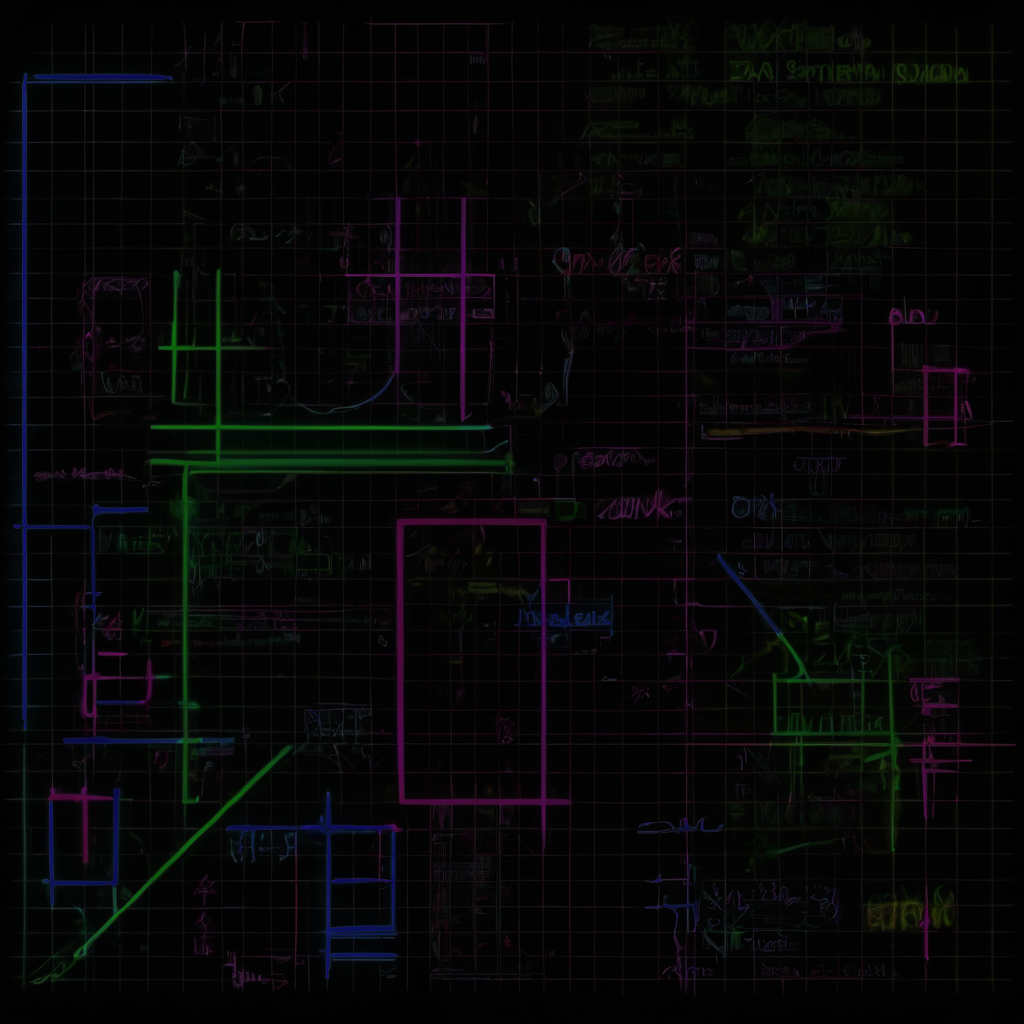
\includegraphics[width=\paperwidth]{fondo}
}
%%%%%%%%%%%%%%%%%%%%%%%%%%%%%%%%%%%%%%%%%%%%%%%%%%%%%%%%%%%%%%%%%%%%%%%%
\usepackage{tikz}
\author{%
Brandon Marquez Salazar
}
\title{%
Patients Bed Positions Classification
Using Pattern Recognition Techniques
}
\date{}
\begin{document}
  \frame{\titlepage}
  \frame{
    \frametitle{Objetive}
    The objective of this experiment is to test pattern recognition
    techniques---LBP in this experiment---and classifiers---such as
    Decision Trees, Bayes Naïve, KNN and SVM---. Also, testing whether
    a good data preprocessing---data augmentation, normalization, 
    balancing, etc.---is required for a better classifier performance.
  }
  \frame{
    \frametitle{Methods}
    In this experiment, the methodology is described below

    \begin{itemize}
      \onslide*<1>{
        \item First version
          \begin{itemize}
            \item Data description
            \item Data loading
            \item Data balancing by undersampling
            \item Feature extraction via LBP
            \item Model selection via Grid Search Cross Validation
            \item Get the best models metrics
          \end{itemize}
        }
      \onslide*<2>{
        \item Second version
          \begin{itemize}
            \item Data description
            \item Data loading
            \item Data balancing by undersampling
            \item Data augmentation using shifting
            \item Feature extraction via LBP
            \item Model selection via Grid Search Cross Validation
            \item Get the best models metrics
          \end{itemize}
        }
    \end{itemize}
  }
  \frame{
    \frametitle{The samples}
    The samples are arrays of pressure levels wich can be interpreted as
    images in 1channel. The documentation gives the dimensions for the image.

    \begin{figure}[!ht]
      \centering
      \tiny
      \begin{subfigure}[t]{0.3\textwidth}
        \centering
        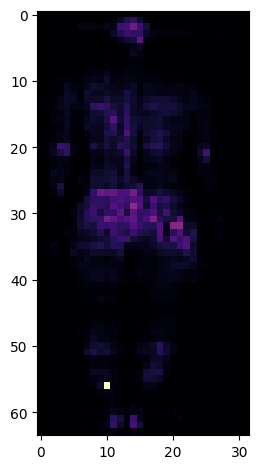
\includegraphics[height=0.45\textheight]{./EI_S1_F1.png}
        \caption{\scriptsize Exp. I, Sam. 1/F.45}
      \end{subfigure}
      \begin{subfigure}[t]{0.3\textwidth}
        \centering
        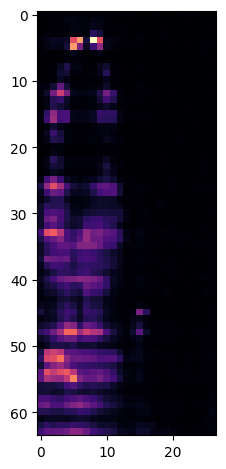
\includegraphics[height=0.45\textheight]{./EII_AirMat_B1.png}
        \caption{\scriptsize Exp. II, Sam. B1/AirMat}
      \end{subfigure}
      \begin{subfigure}[t]{0.33\textwidth}
        \centering
        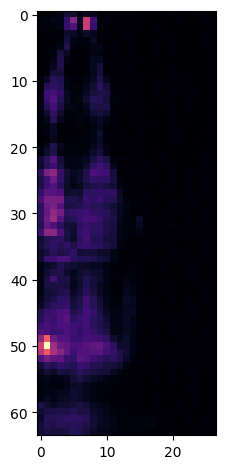
\includegraphics[height=0.45\textheight]{./EII_SpongeMat_B1.png}
        \caption{\scriptsize Exp. II, Sam. B1/SpongeMat}
      \end{subfigure}
    \end{figure}

    \begin{table}[ht]
    \centering
    \begin{minipage}{0.45\textwidth}
      \tiny
      \centering
      \begin{tabular}{|l|c|}
        \hline
        \textbf{Class} & \textbf{Number of Samples} \\
        \hline
        Supine & 10,613 \\
        Right & 4,672 \\
        Left & 4,739 \\
        \hline
        \textbf{Total} & \textbf{20,024} \\
        \hline
      \end{tabular}
      \caption{\scriptsize Class distribution for Exp. I}
      \label{tab:exp1}
    \end{minipage}
    \hfill
    \begin{minipage}{0.45\textwidth}
      \tiny
      \centering
      \begin{tabular}{|l|c|}
        \hline
        \textbf{Class} & \textbf{Number of Samples} \\
        \hline
        Supine & 270 \\
        Right & 144 \\
        Left & 48 \\
        \hline
        \textbf{Total} & \textbf{462} \\
        \hline
      \end{tabular}
      \caption{\scriptsize Class distribution for Exp. II}
      \label{tab:exp2}
    \end{minipage}
    \end{table}
  }
  \frame{
    \frametitle{Data Balancing and Augmentation}

    \onslide*<1>{
      For balancing, the method used was undedrsampling which looks takes
      the cardinalities per class $|\mathcal{C}_i|$ and uses the smallest one
      $N_{\min}$, then, randomizes the samples and piks $N_{\min}$ samples from each
      class, getting the new dataset $\mathcal{S}$.

      \begin{equation*}
        \begin{aligned}
          \mathcal{C} &= \{ \mathcal{C}_1, \mathcal{C}_2, \ldots, \mathcal{C}_n \}\\
          N_{\min} &= \min_{\mathcal{C}_i \in \mathcal{C}} |\mathcal{C}_i|\\
          f&: \mathcal{P}(\mathcal{C}) \times \mathbb{N} \to \mathcal{P}(\mathcal{C})\\
          \mathcal{S} &= \bigcup_{\mathcal{C}_i \in \mathcal{C}} f(\mathcal{C}_i, N_{\min})
        \end{aligned}
      \end{equation*}
    }

    \onslide*<2>{
      Then, for the second version, it was used a data augmentation technique which
      generates new samples by shifting the pixels of the original ones.
      Here, the shifting was made in 4 px---upside and downside, leftside and
      rightside---for $x$ and $y$. With a non destructive shifting.

      \begin{equation*}
        \begin{aligned}
          \text{shift}&: \mathbb{R}^{m \times n} \times \mathbb{Z} \times \mathbb{Z} \to \mathbb{R}^{m \times n}\\
          M_{i+N_{\min}} &= \text{shift}(M_i, x, y)\\
          M_{i+N_{\min}+1} &= \text{shift}(M_i, -x, -y)
        \end{aligned}
      \end{equation*}
    }
  }

  \frame{
    \frametitle{Feature extraction}
    Here, the feature extraction was done via Local Binary Patterns (LBP) which is
    easily defined by

    \begin{equation*}
      \begin{aligned}
        \text{LBP}_{P,R}(x_c, y_c) &= \sum_{p=0}^{P-1} 2^p \cdot [ g_p \geq g_c ]
        \quad \text{where} \quad
        s(x) = \begin{cases}
                 1 & \text{if } x \geq 0 \\
                 0 & \text{otherwise}
               \end{cases}\\
      \end{aligned}
    \end{equation*}

    The LBP was computed for each sample without windowing
    (windowing each sample caused intensive RAM usage).
  }

  \begin{frame}[allowframebreaks]
    \frametitle{Model selection for classification}
    For this, the approach given was Grid Search Cross Validation (GSCV)
    provided by scikit-learn library.
    Here, the main parameters used were:
    % Block 1: Core Classifiers
    \begin{table}[htbp]
      \scriptsize
      \centering
      \caption{Block 1: Core classifiers and their hyperparameter search grids.}
      \label{tab:block1}
      \begin{tabular}{@{}l L l@{}}
      \toprule
      \textbf{Classifier} & \textbf{Hyperparameters} & \textbf{Search Values} \\
      \midrule
      Decision Tree & max\_depth & [3, 5, 7, 10] \\
      & min\_samples\_split & [2, 5, 10] \\
      & criterion & ['gini', 'entropy'] \\
      \midrule
      Random Forest & n\_estimators & [50, 100, 200] \\
      & max\_depth & [3, 5, 7, 10] \\
      & min\_samples\_split & [2, 5, 10] \\
      \midrule
      KNN Coarse & n\_neighbors & [10, 30, 50, 70, 90] \\
      & weights & ['uniform', 'distance'] \\
      \midrule
      AdaBoost & n\_estimators & [50, 100, 200] \\
      & learning\_rate & [0.01, 0.1, 1.0] \\
      \bottomrule
      \end{tabular}
    \end{table}

    % Block 2: KNN Variants
    \begin{table}[htbp]
      \scriptsize
      \centering
      \caption{Block 2: K-Nearest Neighbors variants and their hyperparameter search grids.}
      \label{tab:block2}
      \begin{tabular}{@{}l L l@{}}
      \toprule
      \textbf{Classifier} & \textbf{Hyperparameters} & \textbf{Search Values} \\
      \midrule
      KNN Fine & n\_neighbors & [1, 2, 3] \\
      & weights & ['uniform', 'distance'] \\
      \midrule
      KNN Minkowski & n\_neighbors & [5, 10, 15] \\
      & p (Minkowski param.) & [1, 2, 3] \\
      & weights & ['uniform', 'distance'] \\
      \midrule
      KNN Weighted & n\_neighbors & [5, 10, 15] \\
      & weights & ['distance'] \\
      \midrule
      KNN Medium & n\_neighbors & [10, 15, 20, 25] \\
      & weights & ['uniform', 'distance'] \\
      \bottomrule
      \end{tabular}
    \end{table}

    % Block 3: Probabilistic Classifiers
    \begin{table}[htbp]
      \scriptsize
      \centering
      \caption{Block 3: Probabilistic classifiers and their hyperparameter search grids.}
      \label{tab:block3}
      \begin{tabular}{@{}l L l@{}}
      \toprule
      \textbf{Classifier} & \textbf{Hyperparameters} & \textbf{Search Values} \\
      \midrule
      Naive Bayes (Gaussian) & var\_smoothing & [$1\times10^{-9}$, $1\times10^{-8}$, $1\times10^{-7}$, $1\times10^{-6}$] \\
      \midrule
      LDA & solver & ['svd', 'lsqr', 'eigen'] \\
      & shrinkage & ['auto', 0.1, 0.5, 0.9] \\
      \midrule
      KNN Cosine & n\_neighbors & [5, 10, 15] \\
      & weights & ['uniform', 'distance'] \\
      \bottomrule
      \end{tabular}
    \end{table}

    % Block 4: SVM Classifiers
    \begin{table}[htbp]
      \scriptsize
      \centering
      \caption{Block 4: Support Vector Machine classifiers and their hyperparameter search grids.}
      \label{tab:block4}
      \begin{tabular}{@{}l L l@{}}
      \toprule
      \textbf{Classifier} & \textbf{Hyperparameters} & \textbf{Search Values} \\
      \midrule
      Linear SVM & C (Regularization) & [0.1, 1, 10, 100] \\
                 & kernel & ['linear'] \\
      \midrule
      Quadratic SVM & C (Regularization) & [0.1, 1, 10] \\
                    & degree & [2] \\
                    & gamma & ['scale', 'auto'] \\
      \midrule
      Cubic SVM & C (Regularization) & [0.1, 1, 10] \\
                & degree & [3] \\
                & gamma & ['scale', 'auto'] \\
      \midrule
      Fifth SVM & C (Regularization) & [0.1, 1, 10] \\
                & degree & [5] \\
                & gamma & ['scale', 'auto'] \\
      \bottomrule
      \end{tabular}
    \end{table}
  \end{frame}

    \begin{frame}{Experimental Results Summary}
      \framesubtitle{Performance metrics across all blocks and experiments}
      \centering

      % Scale the table to fit the frame width
      \resizebox{\textwidth}{!}{%
        \begin{tabular}{@{} l l *{5}{S[table-format=1.3]} S[table-format=1.4] S[table-format=1.3] @{}}
          \toprule
          \multirow{2}{*}{\textbf{Experiment}} & \multirow{2}{*}{\textbf{Best Model}} & \textbf{Acc.} & \textbf{Prec.} & \textbf{Rec.} & \textbf{F1} & \textbf{AUC} & \textbf{CV} \\
           & & & & & & \textbf{Score} & \textbf{Score} \\
          \midrule
          \multicolumn{8}{l}{\textbf{Experiment I}} \\
          \midrule
          Block 1: Tree-Based & KNN Coarse & 0.8734 & 0.8733 & 0.8734 & 0.8733 & 0.9676 & 0.8639 \\
          Block 2: KNN Variants & KNN Medium & 0.8734 & 0.8733 & 0.8734 & 0.8733 & 0.9676 & 0.8639 \\
          Block 3: Probabilistic & KNN Cosine & 0.8146 & 0.8156 & 0.8146 & 0.8144 & 0.9439 & 0.8160 \\
          Block 4: SVM Variants & Quadratic SVM & 0.6555 & 0.6612 & 0.6555 & 0.6460 & {N/A} & 0.6540 \\
          \midrule
          \multicolumn{8}{l}{\textbf{Experiment II}} \\
          \midrule
          Block 1: Tree-Based & Decision Tree & 0.5172 & 0.5157 & 0.5172 & 0.4937 & 0.6558 & 0.5391 \\
          Block 2: KNN Variants & KNN Fine & 0.5172 & 0.5640 & 0.5172 & 0.4875 & 0.6849 & 0.5304 \\
          Block 3: Probabilistic & KNN Cosine & 0.5517 & 0.5552 & 0.5517 & 0.5526 & 0.7247 & 0.4609 \\
          Block 4: SVM Variants & Linear SVM & 0.5517 & 0.5699 & 0.5517 & 0.5507 & {N/A} & 0.4348 \\
          \bottomrule
        \end{tabular}%
      }

      \vspace{1em}
      \footnotesize \textit{Note:} Acc. = Accuracy, Prec. = Precision, Rec. = Recall, CV = Cross-Validation.\\
      N/A indicates the metric was not available for that model.
    \end{frame}

    \begin{frame}{Impact of Data Augmentation on Model Performance}
      \framesubtitle{Comparative results before and after augmentation}
      \centering

      \resizebox{\textwidth}{!}{%
        \begin{tabular}{@{} l l *{5}{S[table-format=1.3]} S[table-format=1.4] S[table-format=1.3] @{}}
          \toprule
          \multirow{2}{*}{\textbf{Experiment}} & \multirow{2}{*}{\textbf{Best Model}} & \textbf{Acc.} & \textbf{Prec.} & \textbf{Rec.} & \textbf{F1} & \textbf{AUC} & \textbf{CV} \\
           & & & & & & \textbf{Score} & \textbf{Score} \\
          \midrule
          \multicolumn{7}{l}{\textbf{Without Data Augmentation (Experiment I)}} \\
          \midrule
          Tree-Based & KNN Coarse & 0.873 & 0.873 & 0.873 & 0.873 & 0.968 & 0.864 \\
          KNN Variants & KNN Medium & 0.873 & 0.873 & 0.873 & 0.873 & 0.968 & 0.864 \\
          Probabilistic & KNN Cosine & 0.814 & 0.815 & 0.814 & 0.814 & 0.944 & 0.816 \\
          SVM Variants & Quadratic SVM & 0.655 & 0.661 & 0.655 & 0.646 & {N/A} & 0.654 \\
          \midrule
          \multicolumn{7}{l}{\textbf{With Data Augmentation (Experiment II)}} \\
          \midrule
          Tree-Based & Decision Tree & 0.517 & 0.516 & 0.517 & 0.494 & 0.656 & 0.539 \\
          KNN Variants & KNN Fine & 0.517 & 0.564 & 0.517 & 0.487 & 0.685 & 0.530 \\
          Probabilistic & KNN Cosine & 0.552 & 0.555 & 0.552 & 0.553 & 0.725 & 0.461 \\
          SVM Variants & Linear SVM & 0.552 & 0.570 & 0.552 & 0.551 & {N/A} & 0.435 \\
          \bottomrule
        \end{tabular}%
      }

      \vspace{1em}
      \footnotesize
      \textit{Note:} Acc. = Accuracy, Prec. = Precision, Rec. = Recall, CV = Cross-Validation Score.\\
      Results show significant performance difference between augmented and non-augmented datasets.
    \end{frame}

    % ==================== EXPERIMENT I PLOTS ====================
% Block 1: Tree-Based (Experiment I)
    \begin{frame}{Block 1: Tree-Based Classifiers (Experiment I)}
    \framesubtitle{Best Model: KNN Coarse}
    \begin{columns}
        \begin{column}{0.33\textwidth}
            \centering
            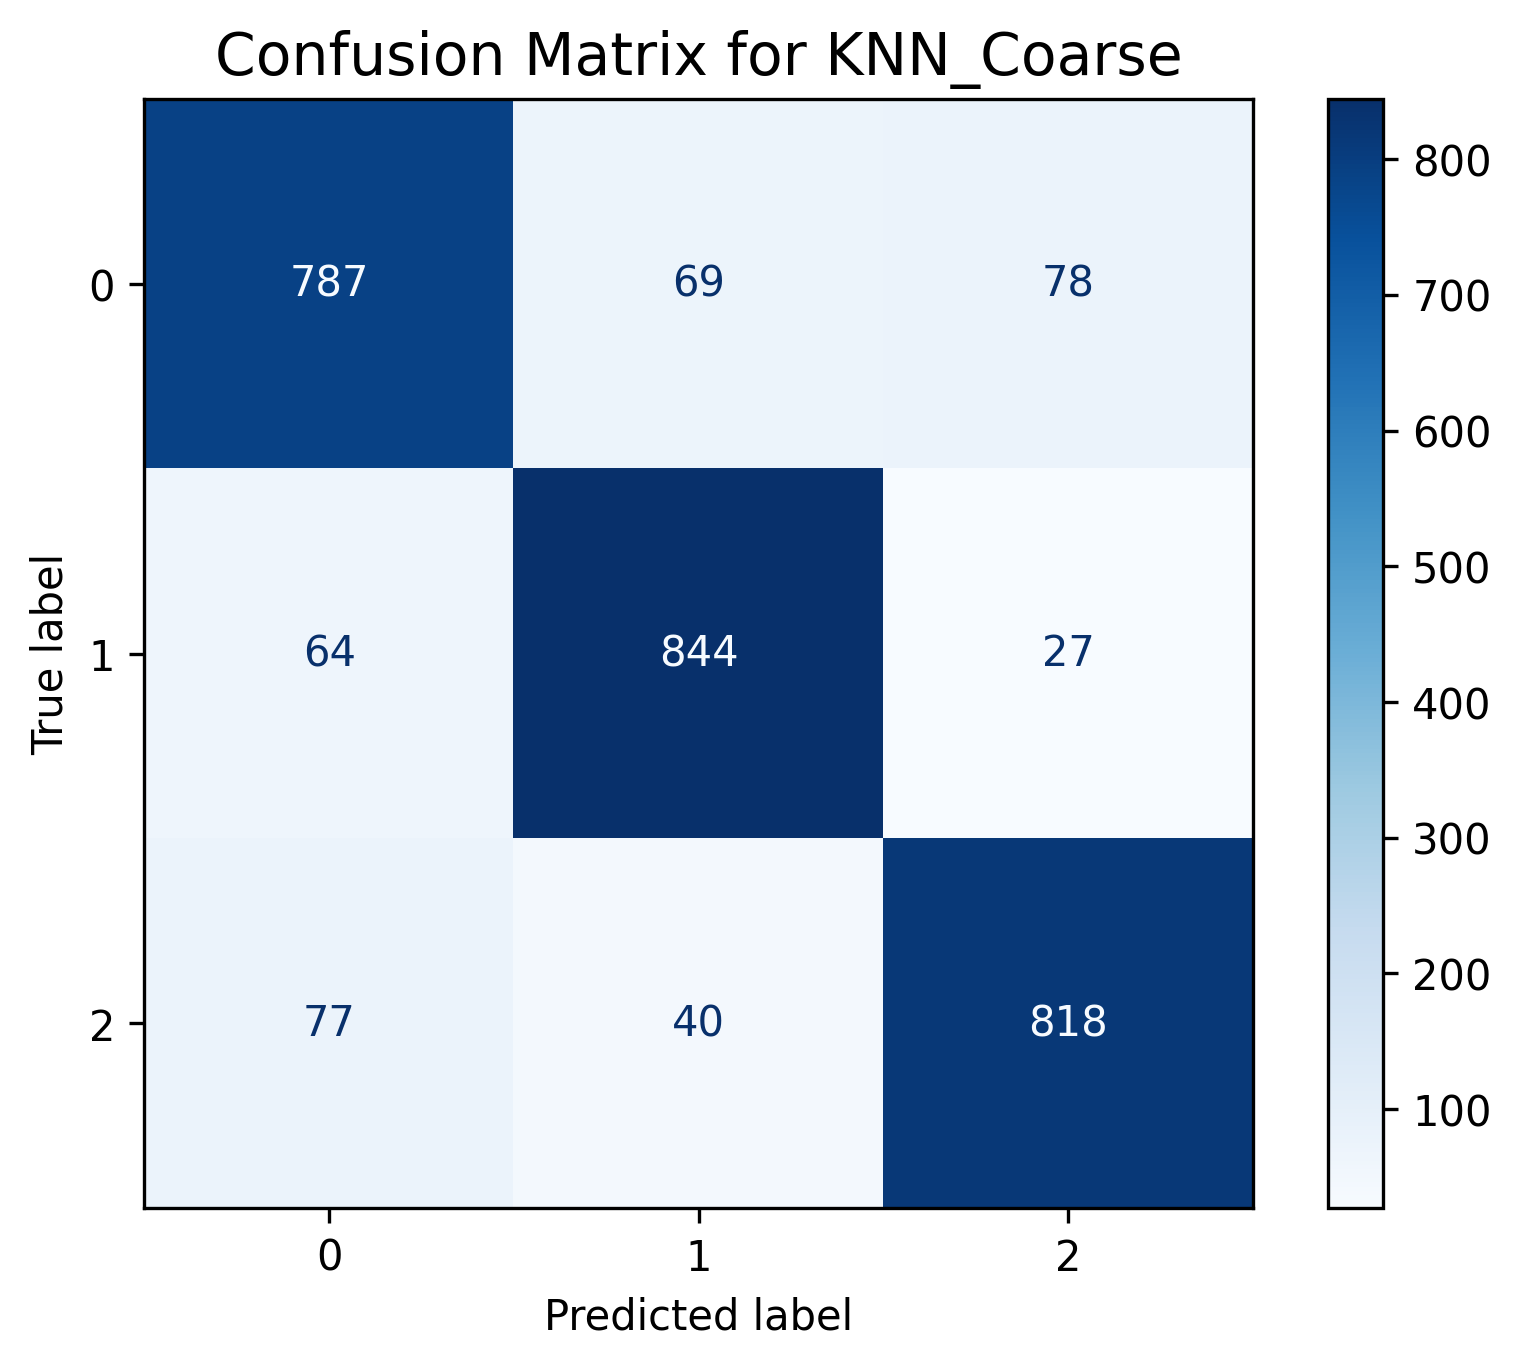
\includegraphics[width=\textwidth]{code/ResultsMainAugZip/plots/Block1_Tree_Based_Experiment_I/confusion_matrix_KNN_Coarse.png}
            \captionof{figure}{Confusion Matrix}
        \end{column}
        \begin{column}{0.33\textwidth}
            \centering
            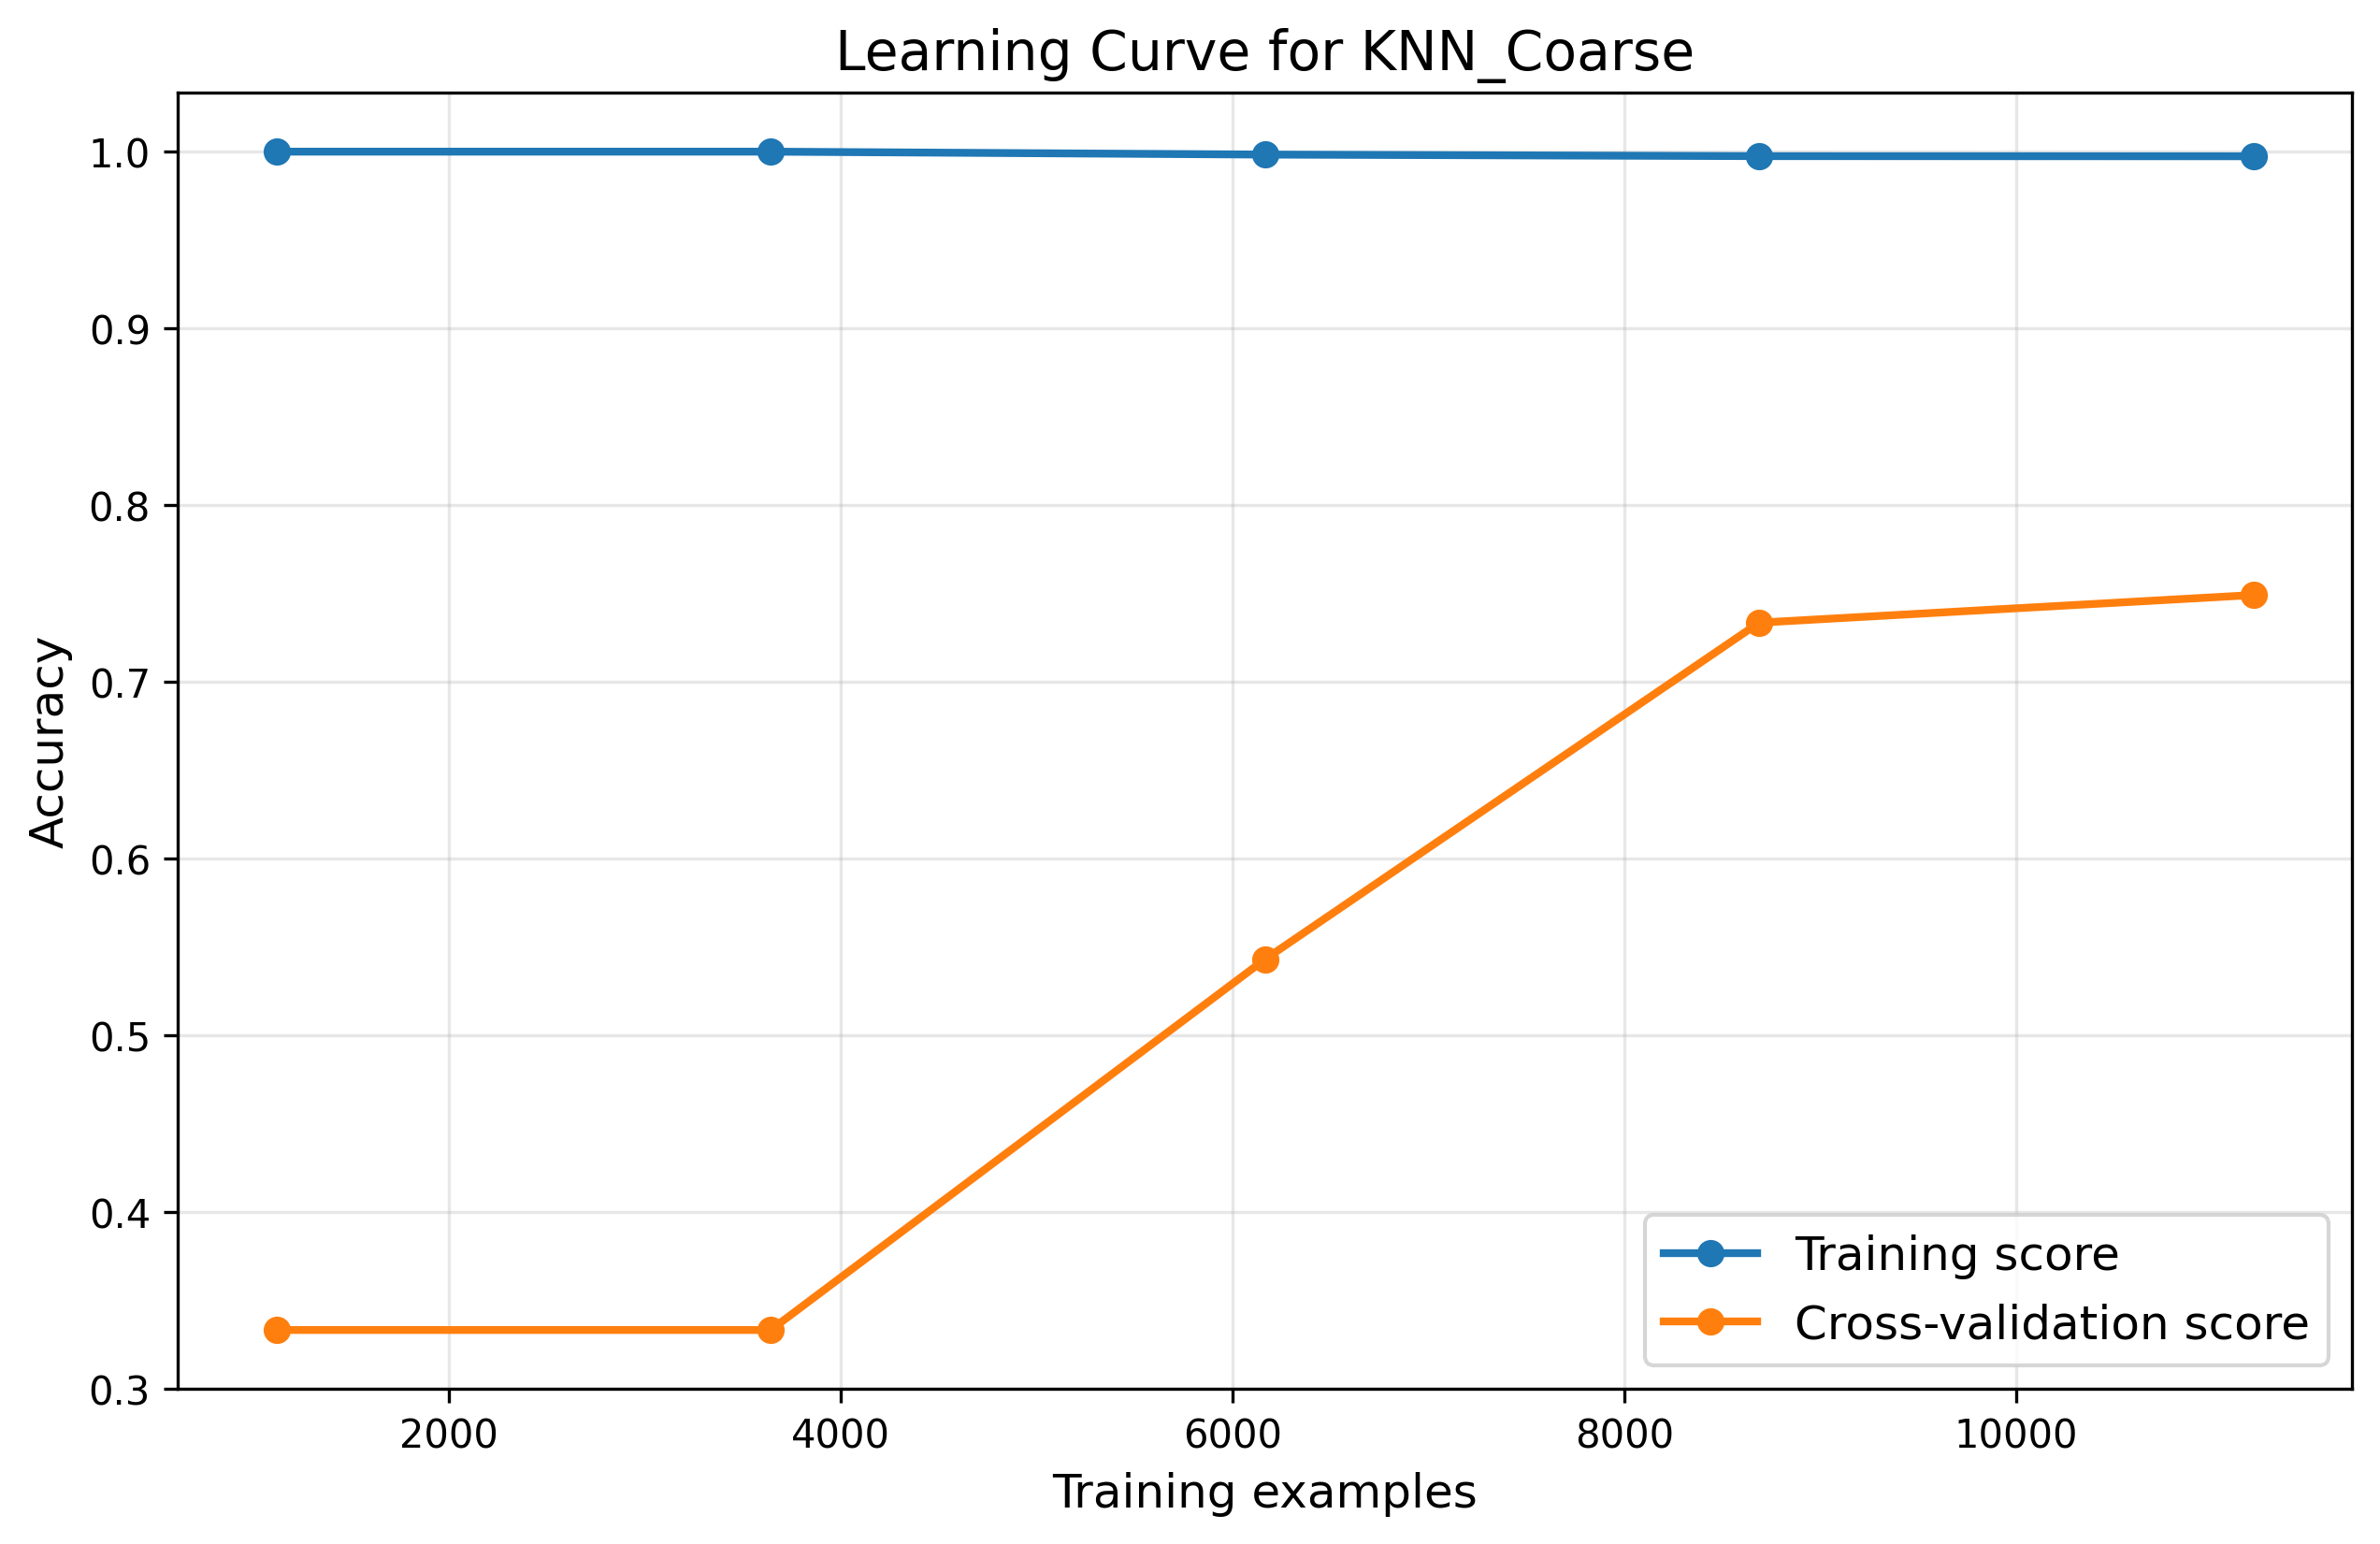
\includegraphics[width=\textwidth]{code/ResultsMainAugZip/plots/Block1_Tree_Based_Experiment_I/learning_curve_KNN_Coarse.png}
            \captionof{figure}{Learning Curve}
        \end{column}
        \begin{column}{0.33\textwidth}
            \centering
            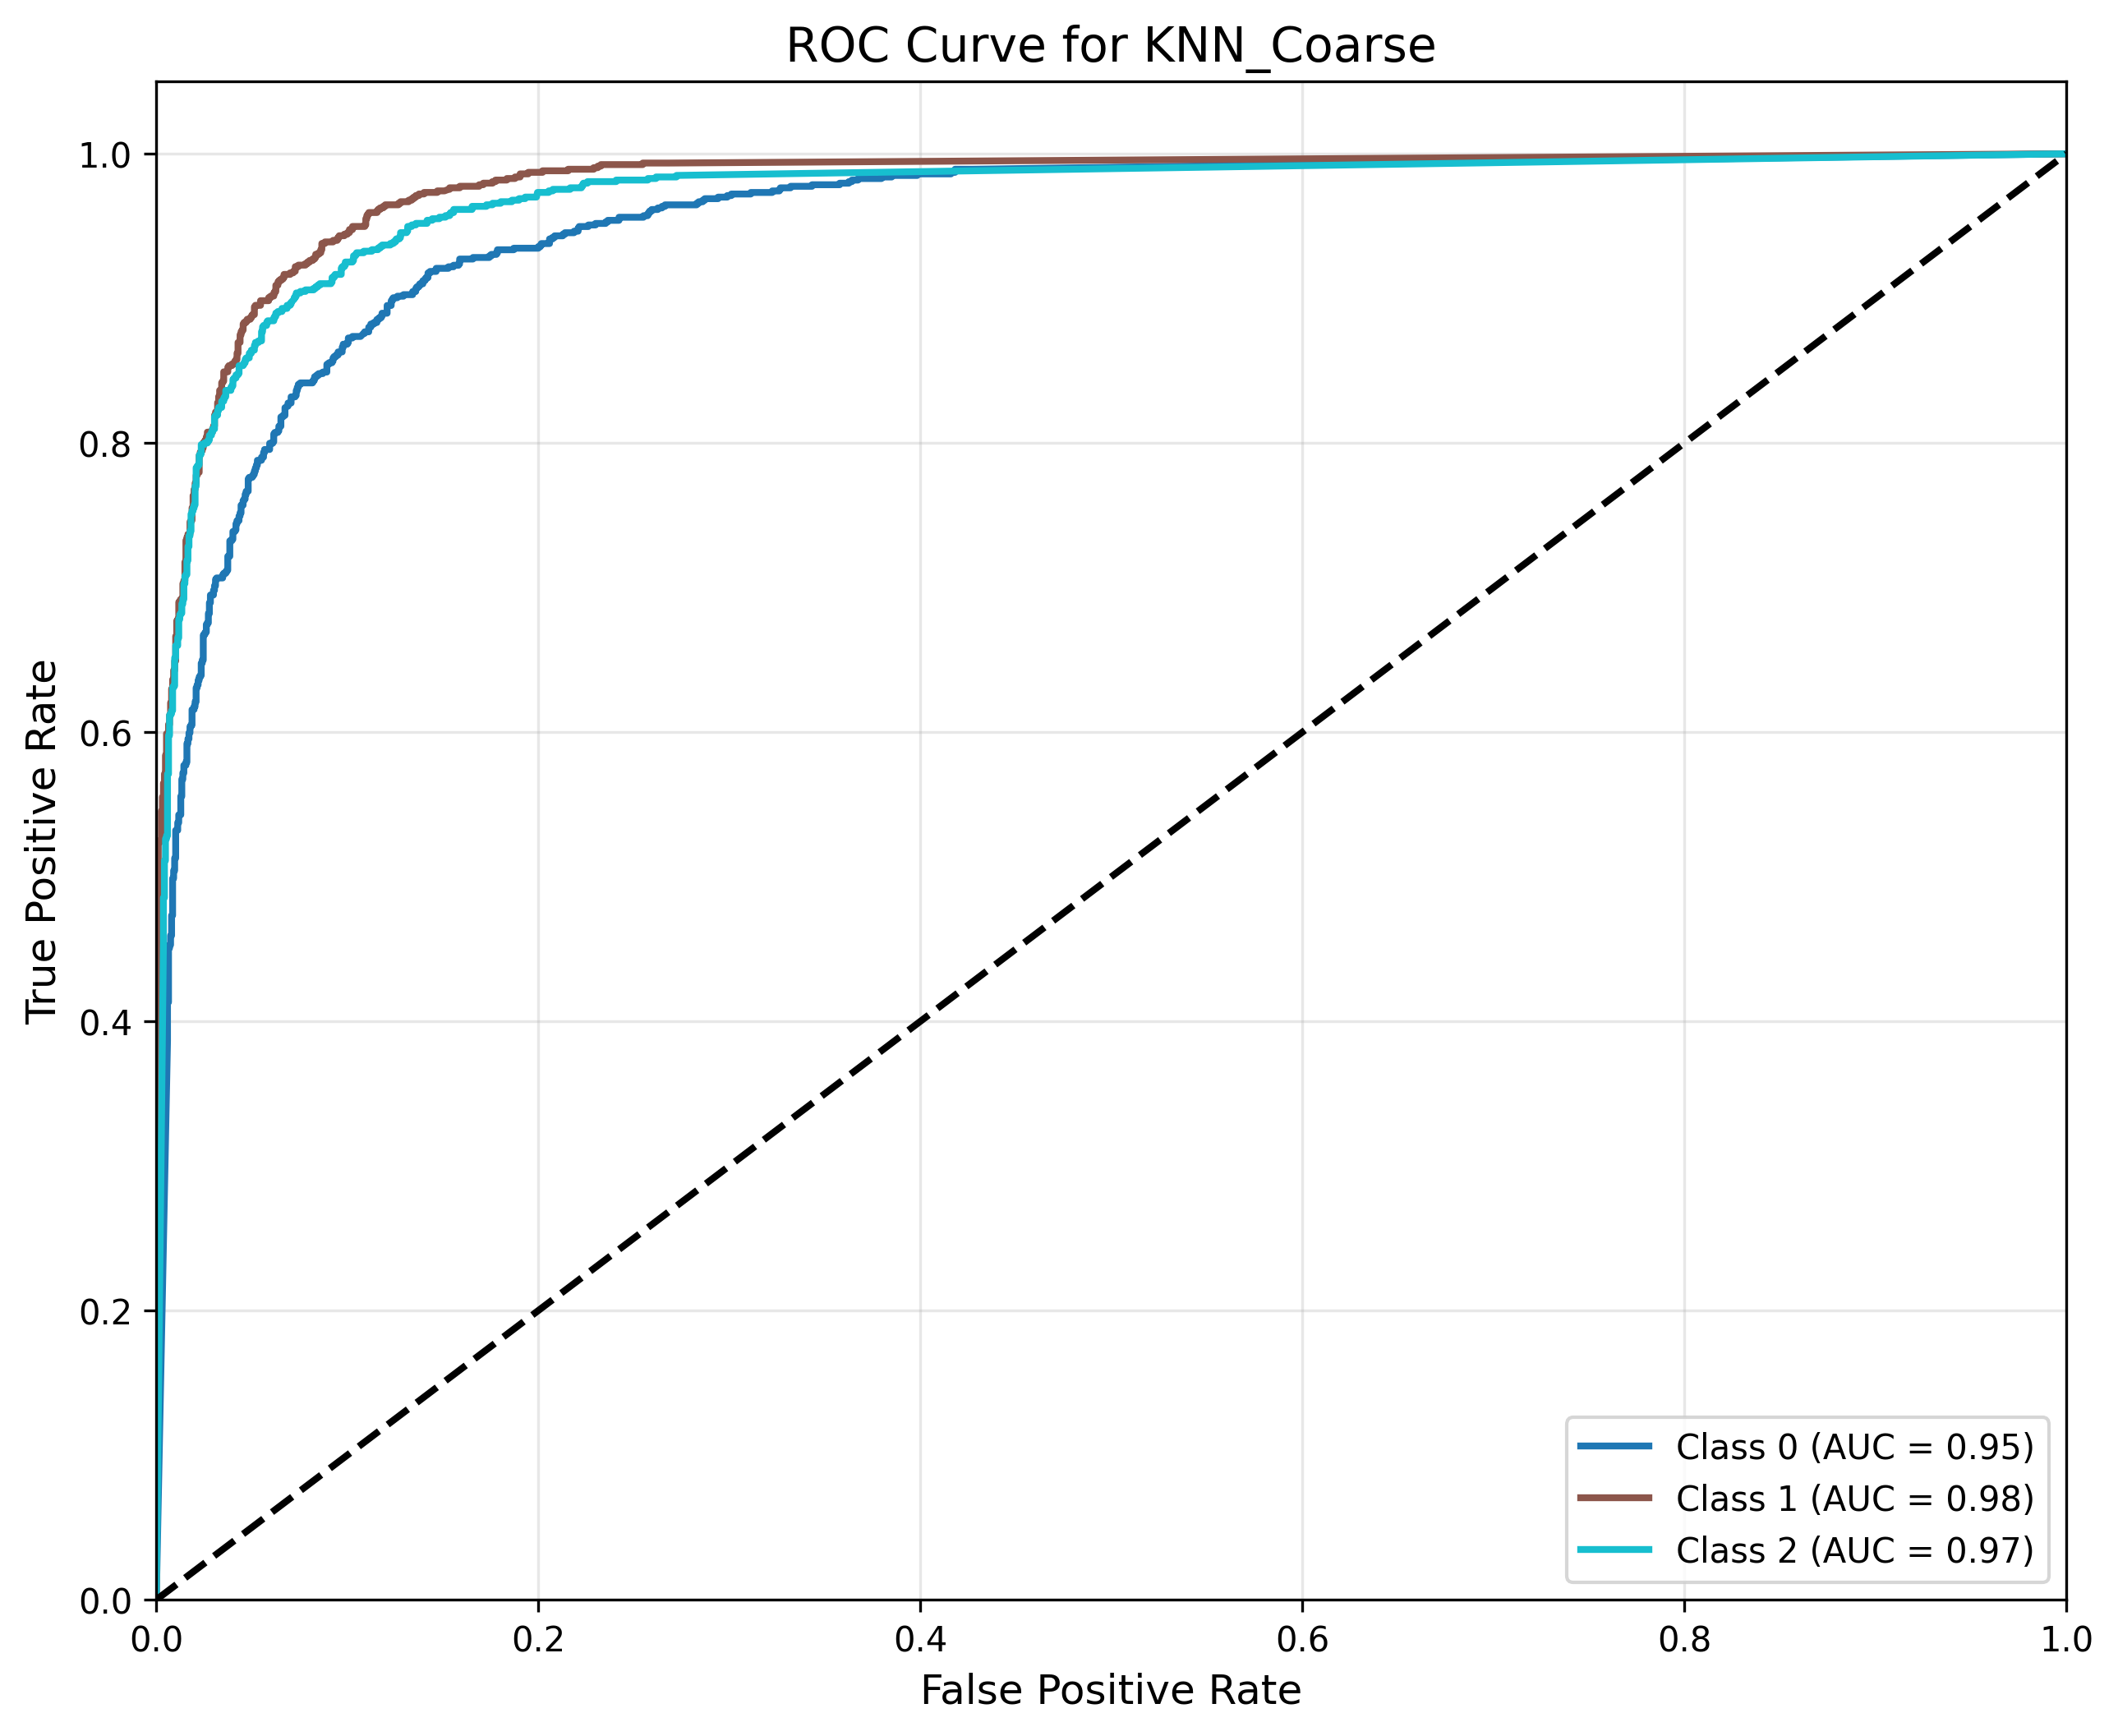
\includegraphics[width=\textwidth]{code/ResultsMainAugZip/plots/Block1_Tree_Based_Experiment_I/roc_curve_KNN_Coarse.png}
            \captionof{figure}{ROC Curve}
        \end{column}
    \end{columns}
    \end{frame}
    
    % Block 2: KNN Variants (Experiment I)
    \begin{frame}{Block 2: KNN Variants (Experiment I)}
    \framesubtitle{Best Model: KNN Medium}
    \begin{columns}
        \begin{column}{0.33\textwidth}
            \centering
            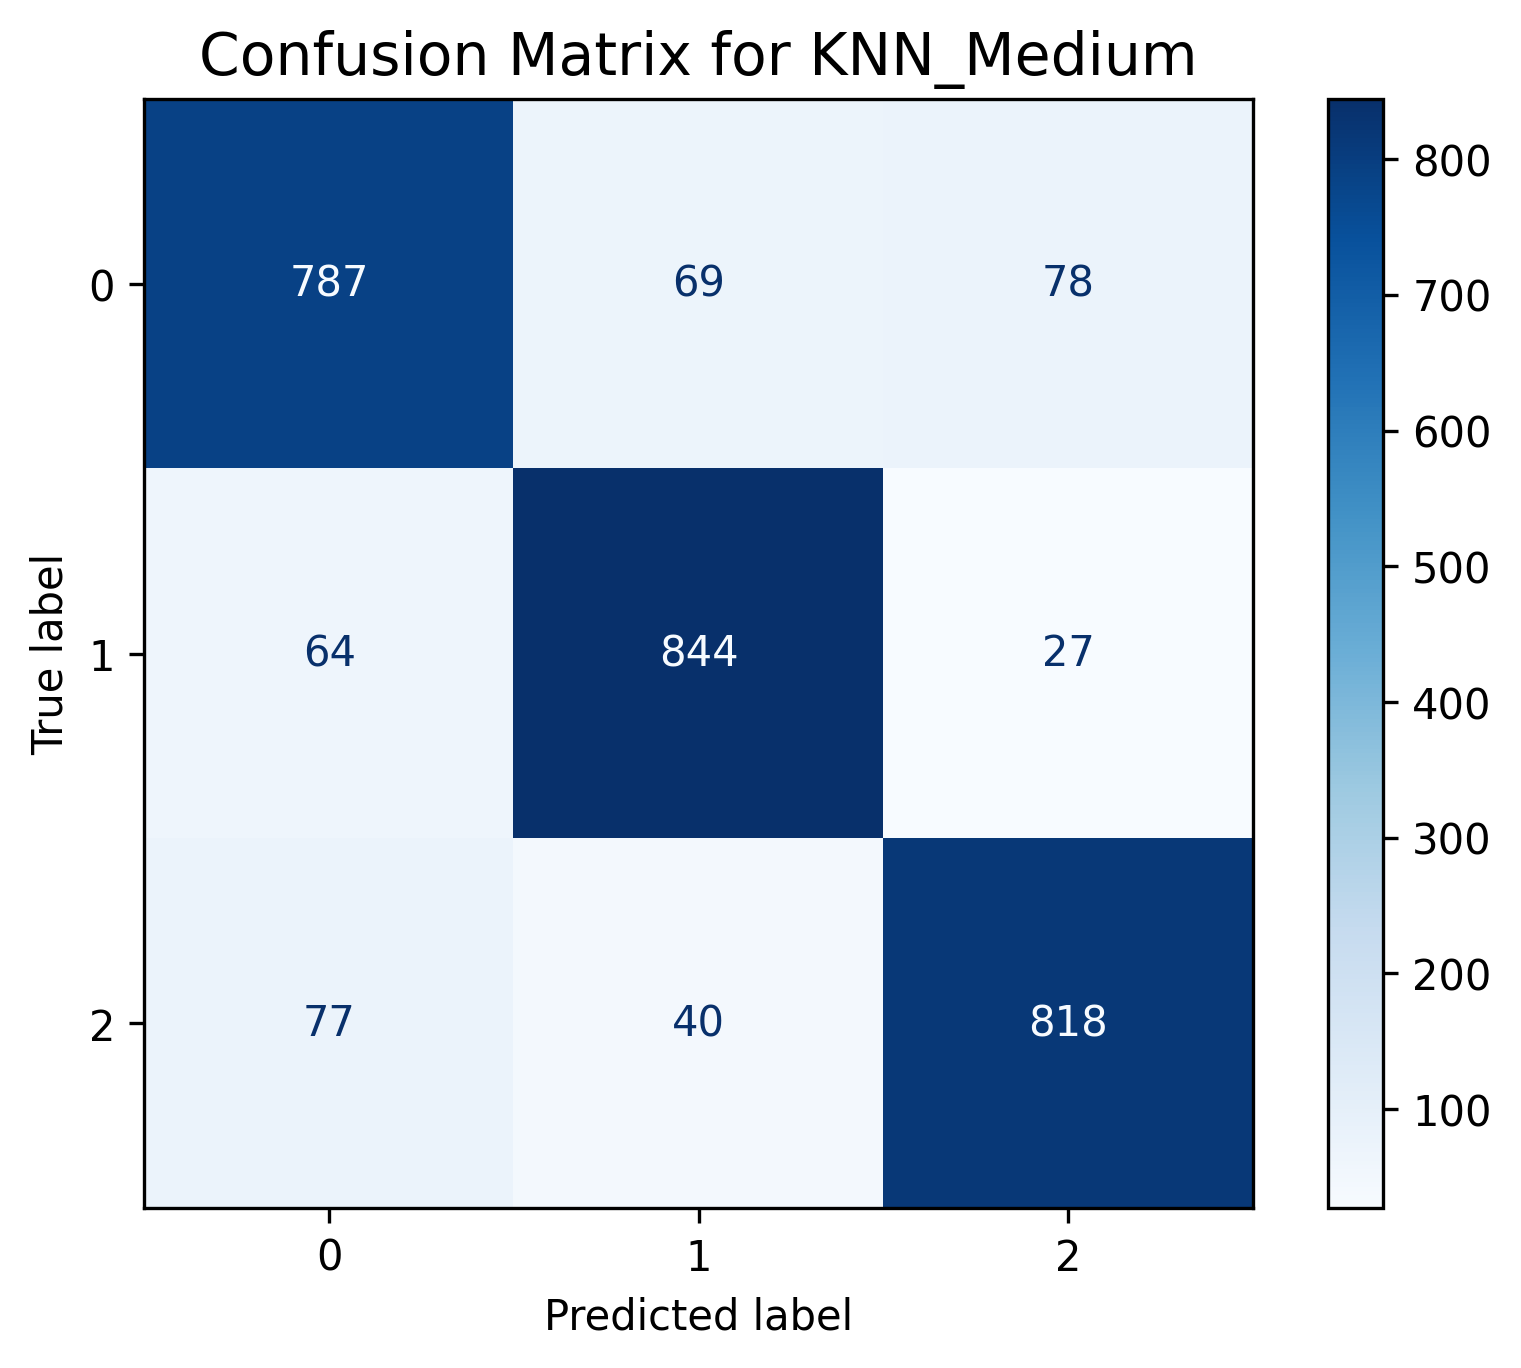
\includegraphics[width=\textwidth]{code/ResultsMainAugZip/plots/Block2_KNN_Variants_Experiment_I/confusion_matrix_KNN_Medium.png}
            \captionof{figure}{Confusion Matrix}
        \end{column}
        \begin{column}{0.33\textwidth}
            \centering
            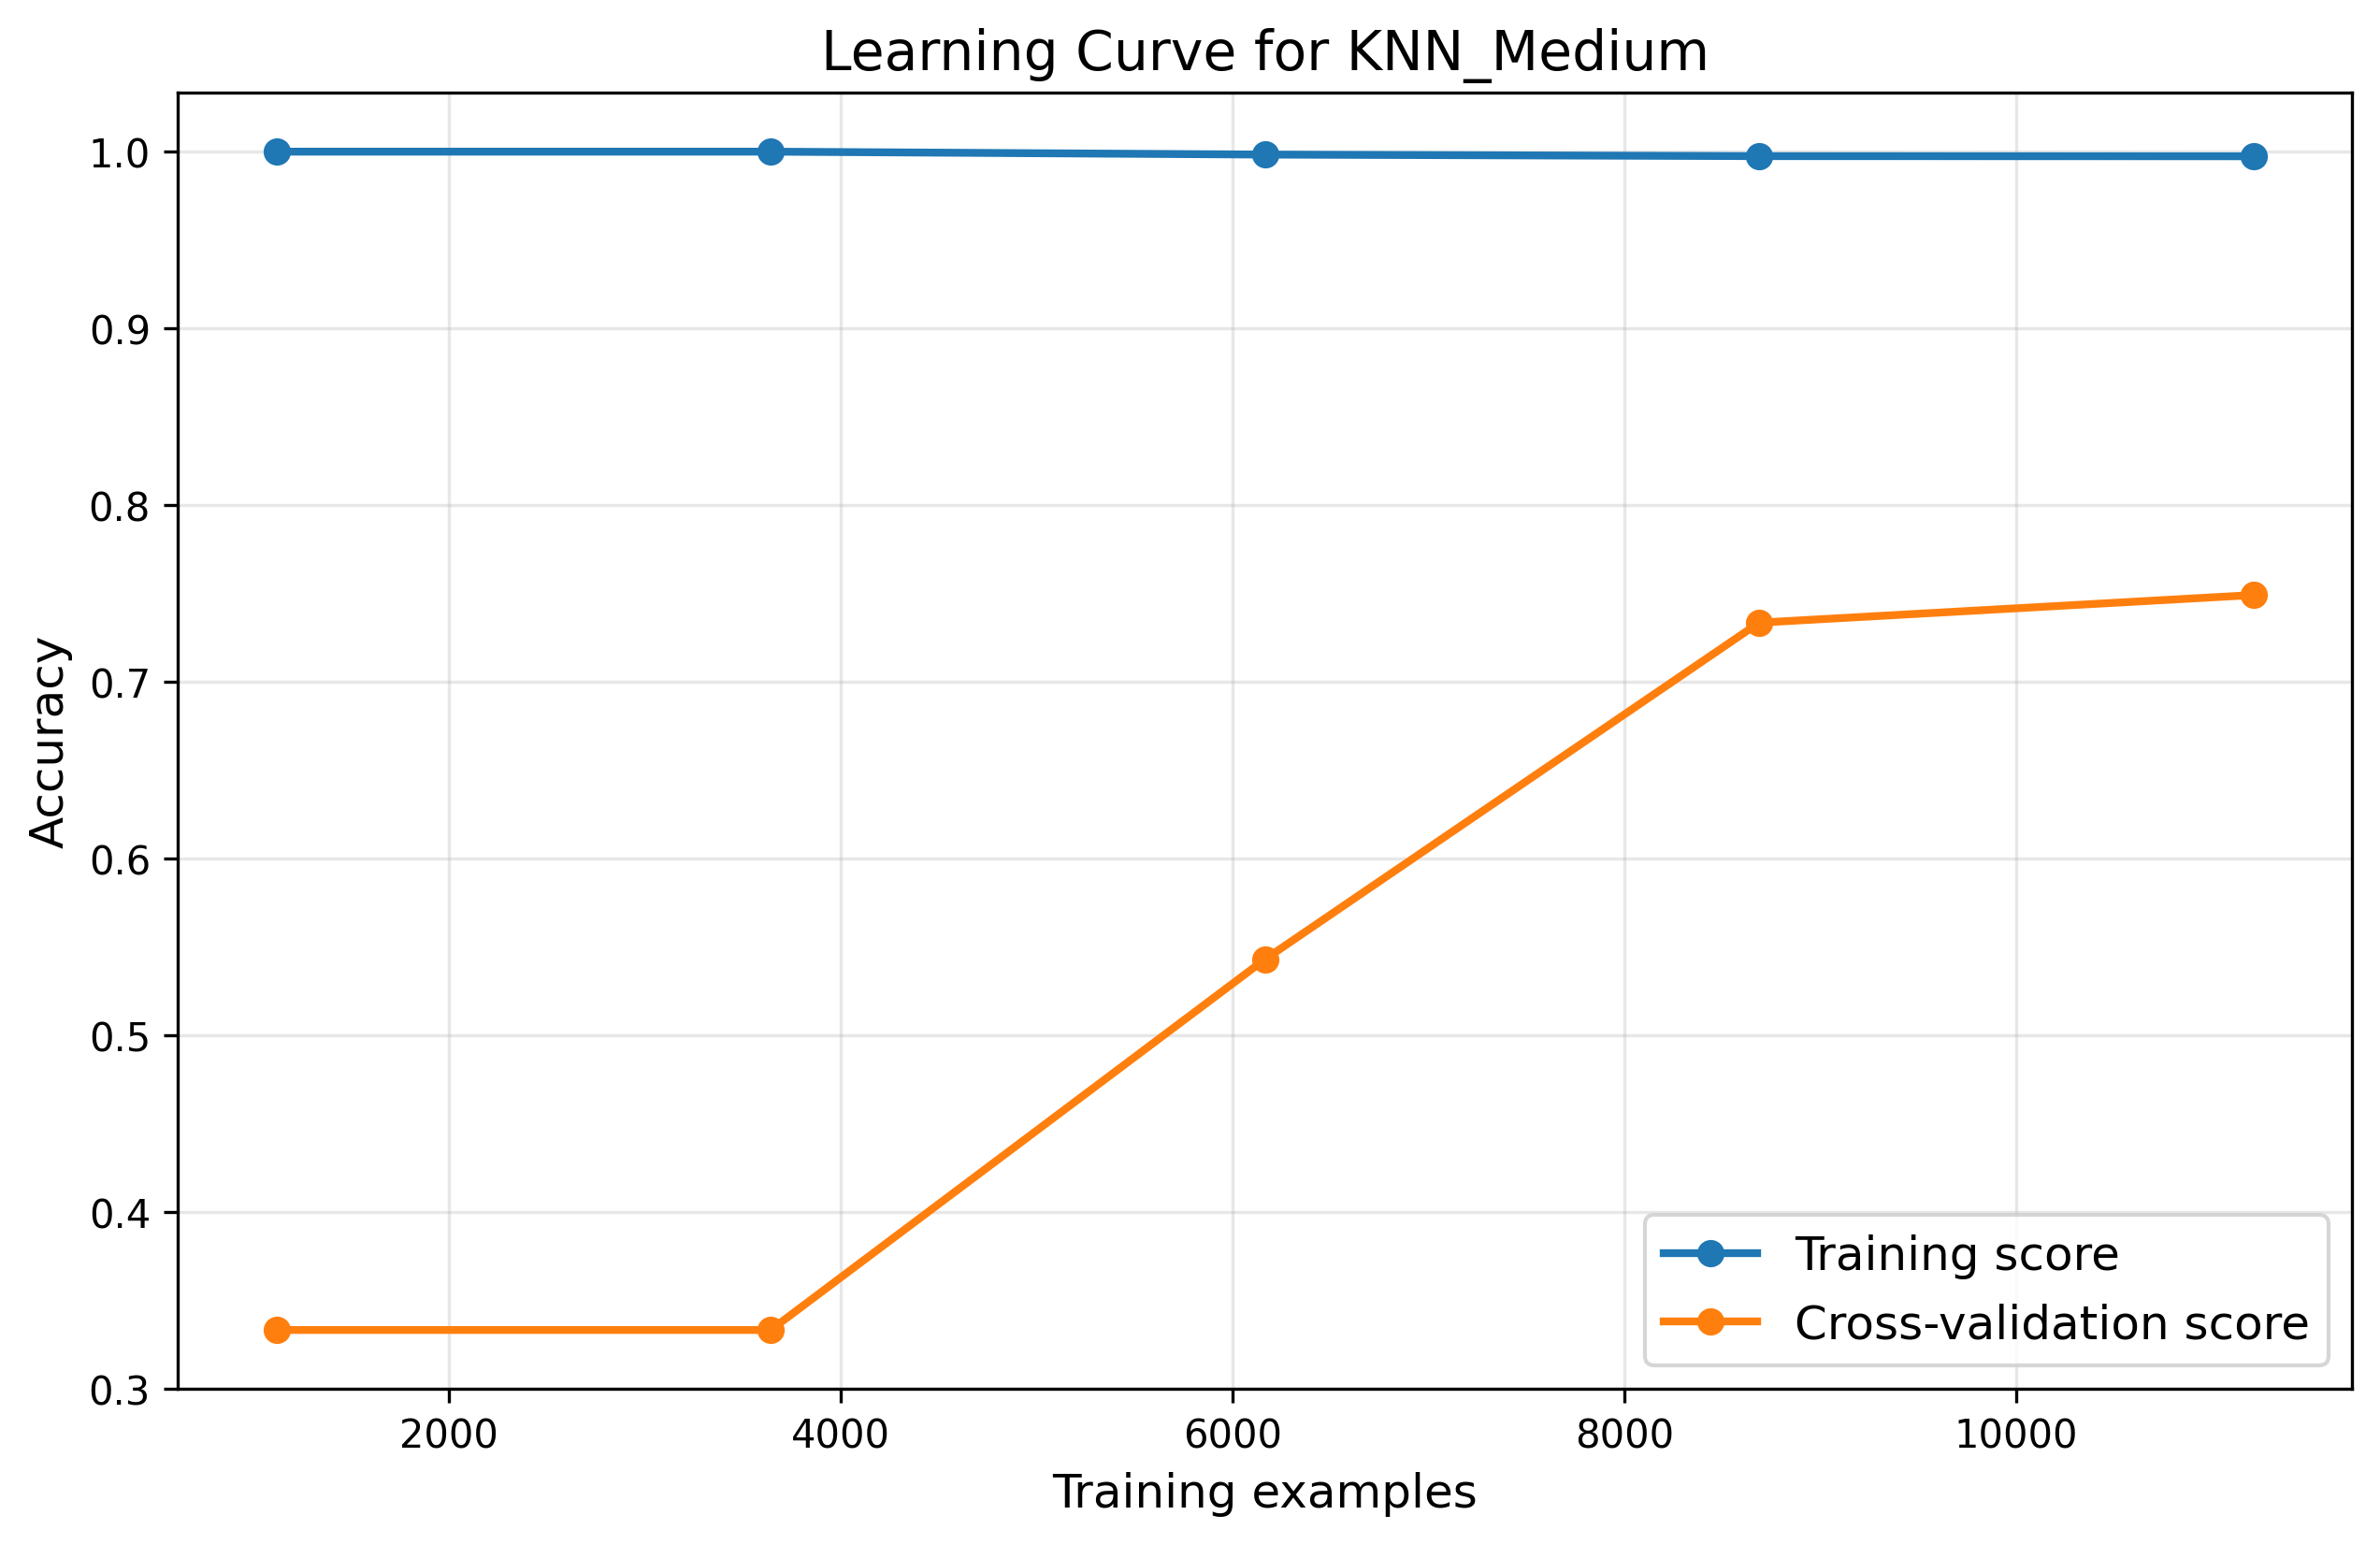
\includegraphics[width=\textwidth]{code/ResultsMainAugZip/plots/Block2_KNN_Variants_Experiment_I/learning_curve_KNN_Medium.png}
            \captionof{figure}{Learning Curve}
        \end{column}
        \begin{column}{0.33\textwidth}
            \centering
            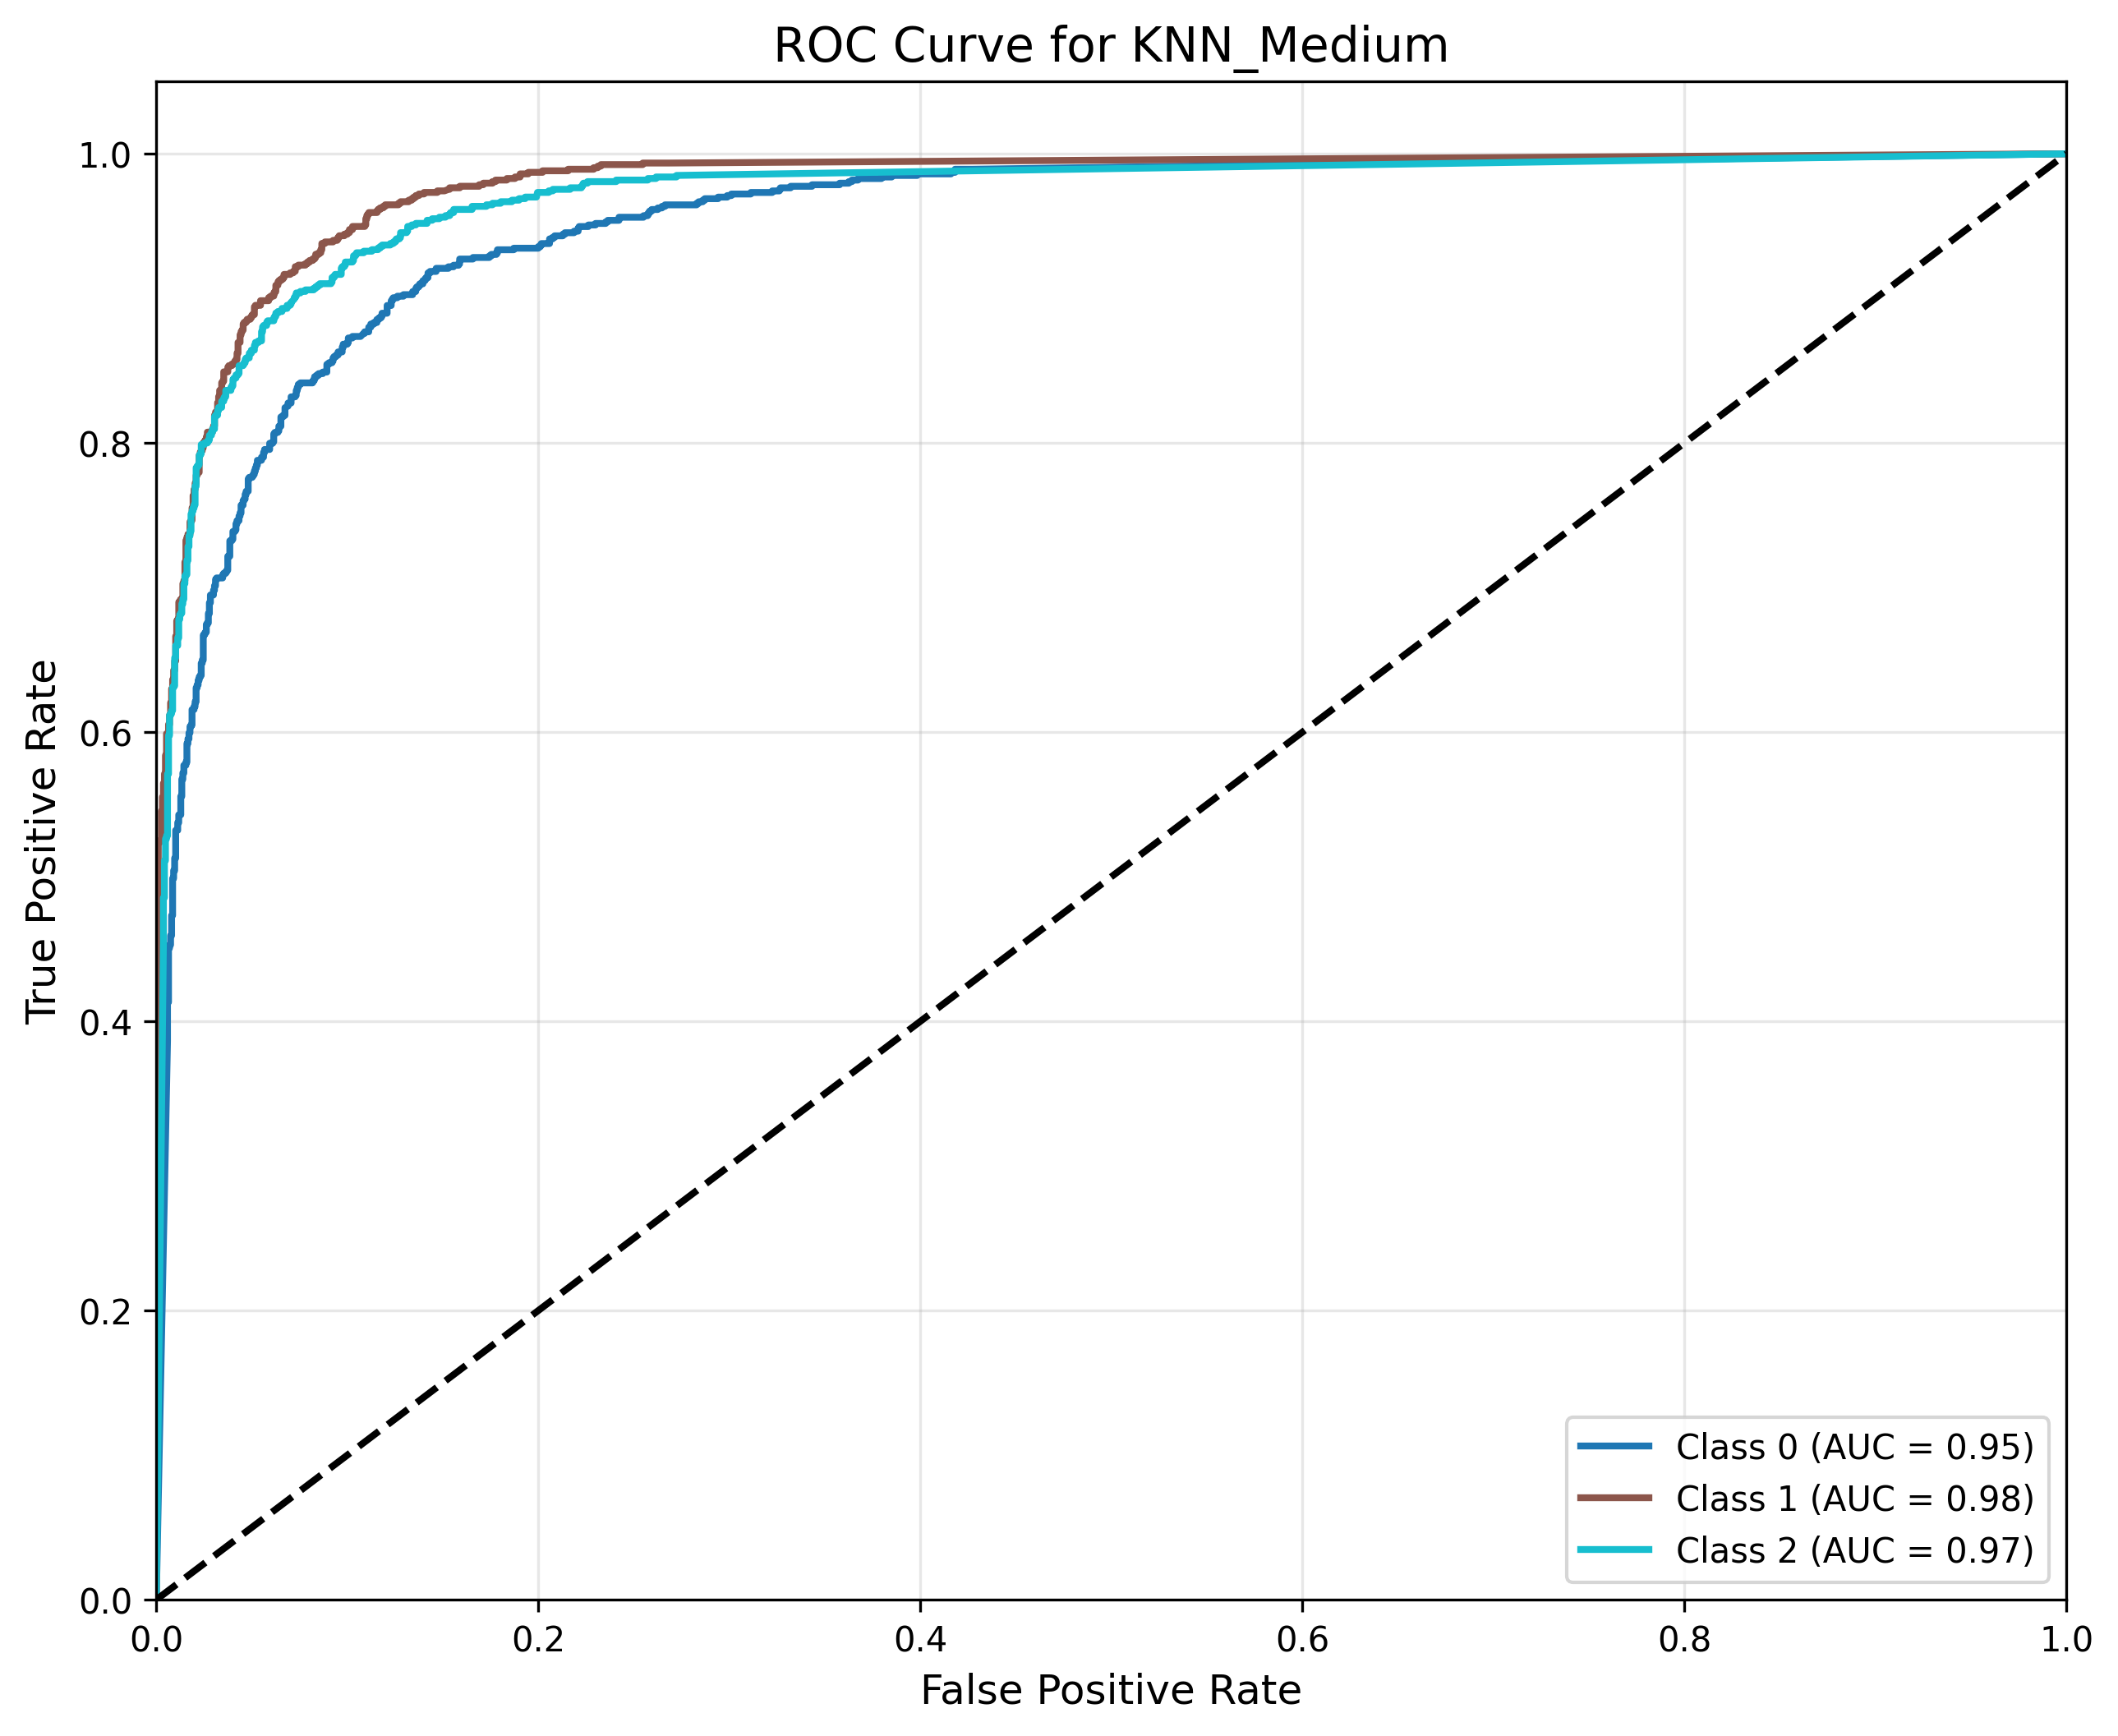
\includegraphics[width=\textwidth]{code/ResultsMainAugZip/plots/Block2_KNN_Variants_Experiment_I/roc_curve_KNN_Medium.png}
            \captionof{figure}{ROC Curve}
        \end{column}
    \end{columns}
    \end{frame}
    
    % Block 3: Probabilistic (Experiment I)
    \begin{frame}{Block 3: Probabilistic Classifiers (Experiment I)}
    \framesubtitle{Best Model: KNN Cosine}
    \begin{columns}
        \begin{column}{0.33\textwidth}
            \centering
            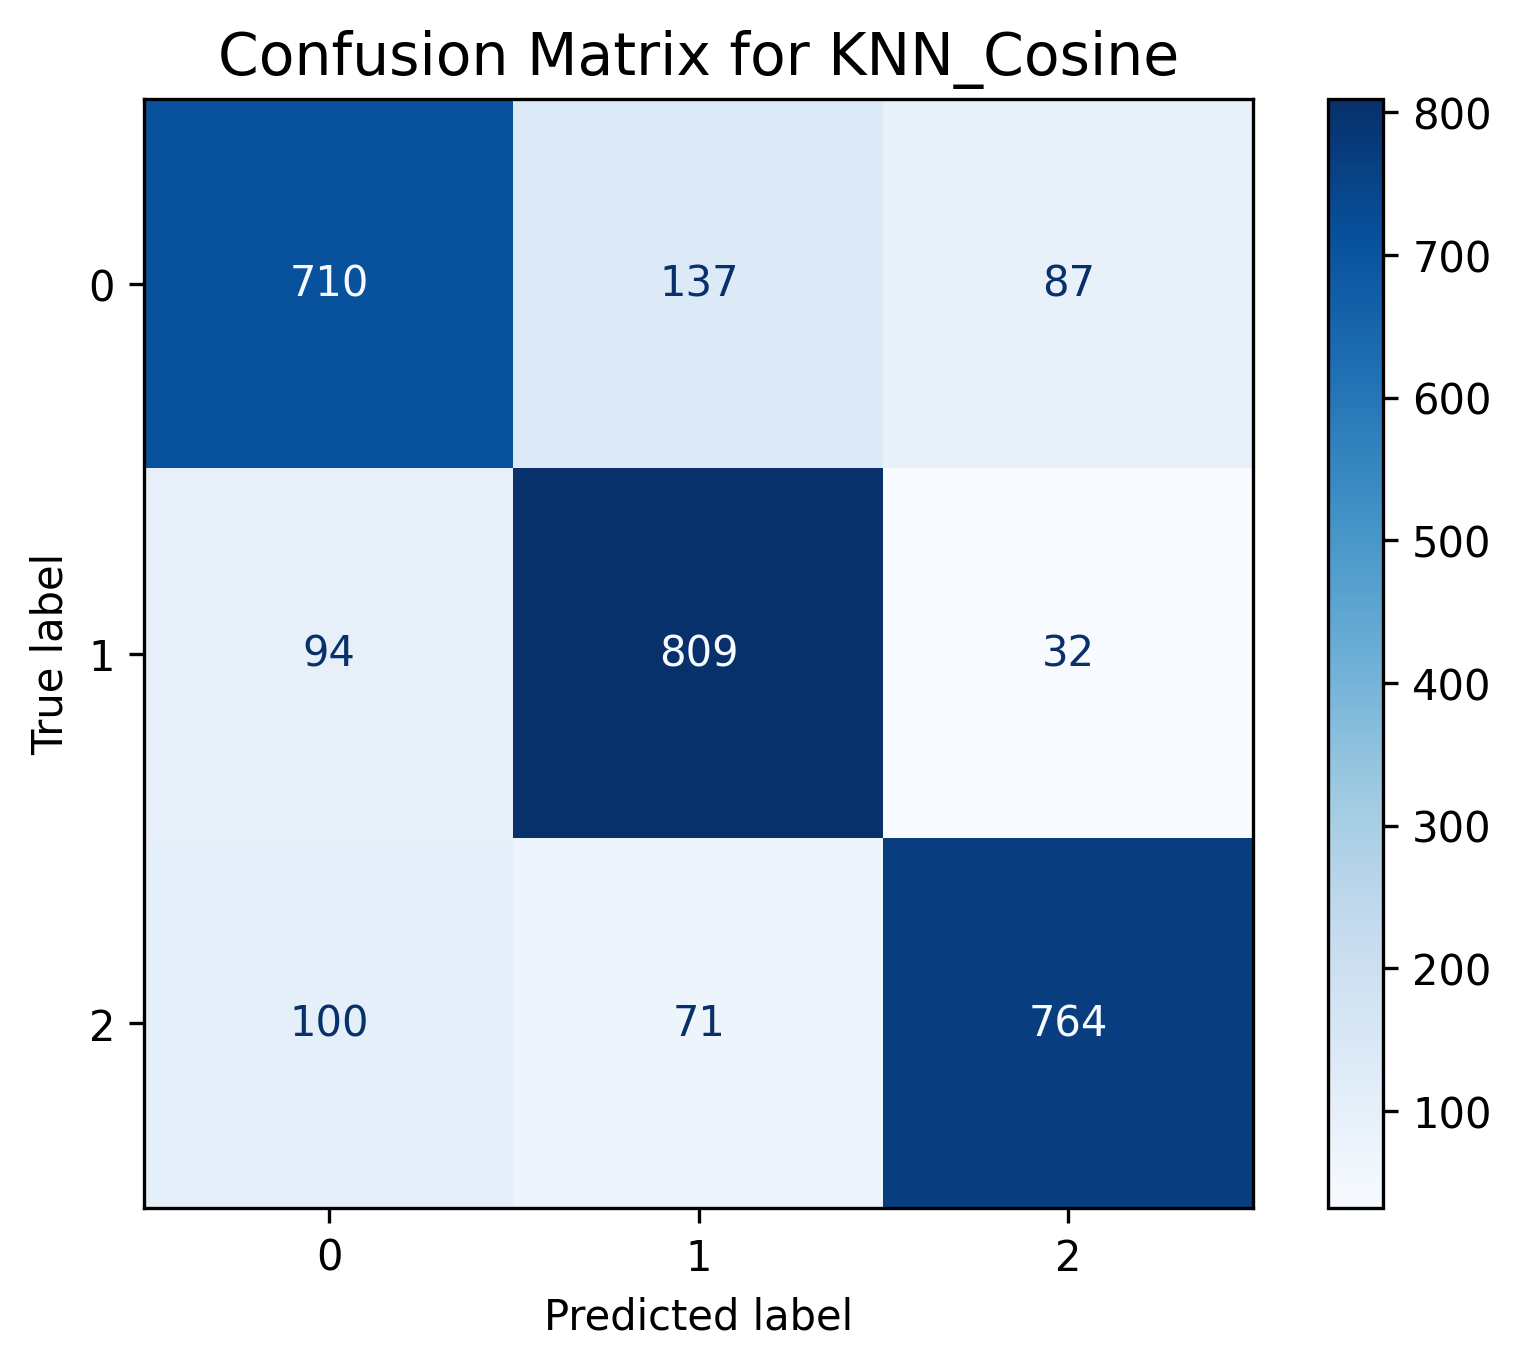
\includegraphics[width=\textwidth]{code/ResultsMainAugZip/plots/Block3_Probabilistic_Experiment_I/confusion_matrix_KNN_Cosine.png}
            \captionof{figure}{Confusion Matrix}
        \end{column}
        \begin{column}{0.33\textwidth}
            \centering
            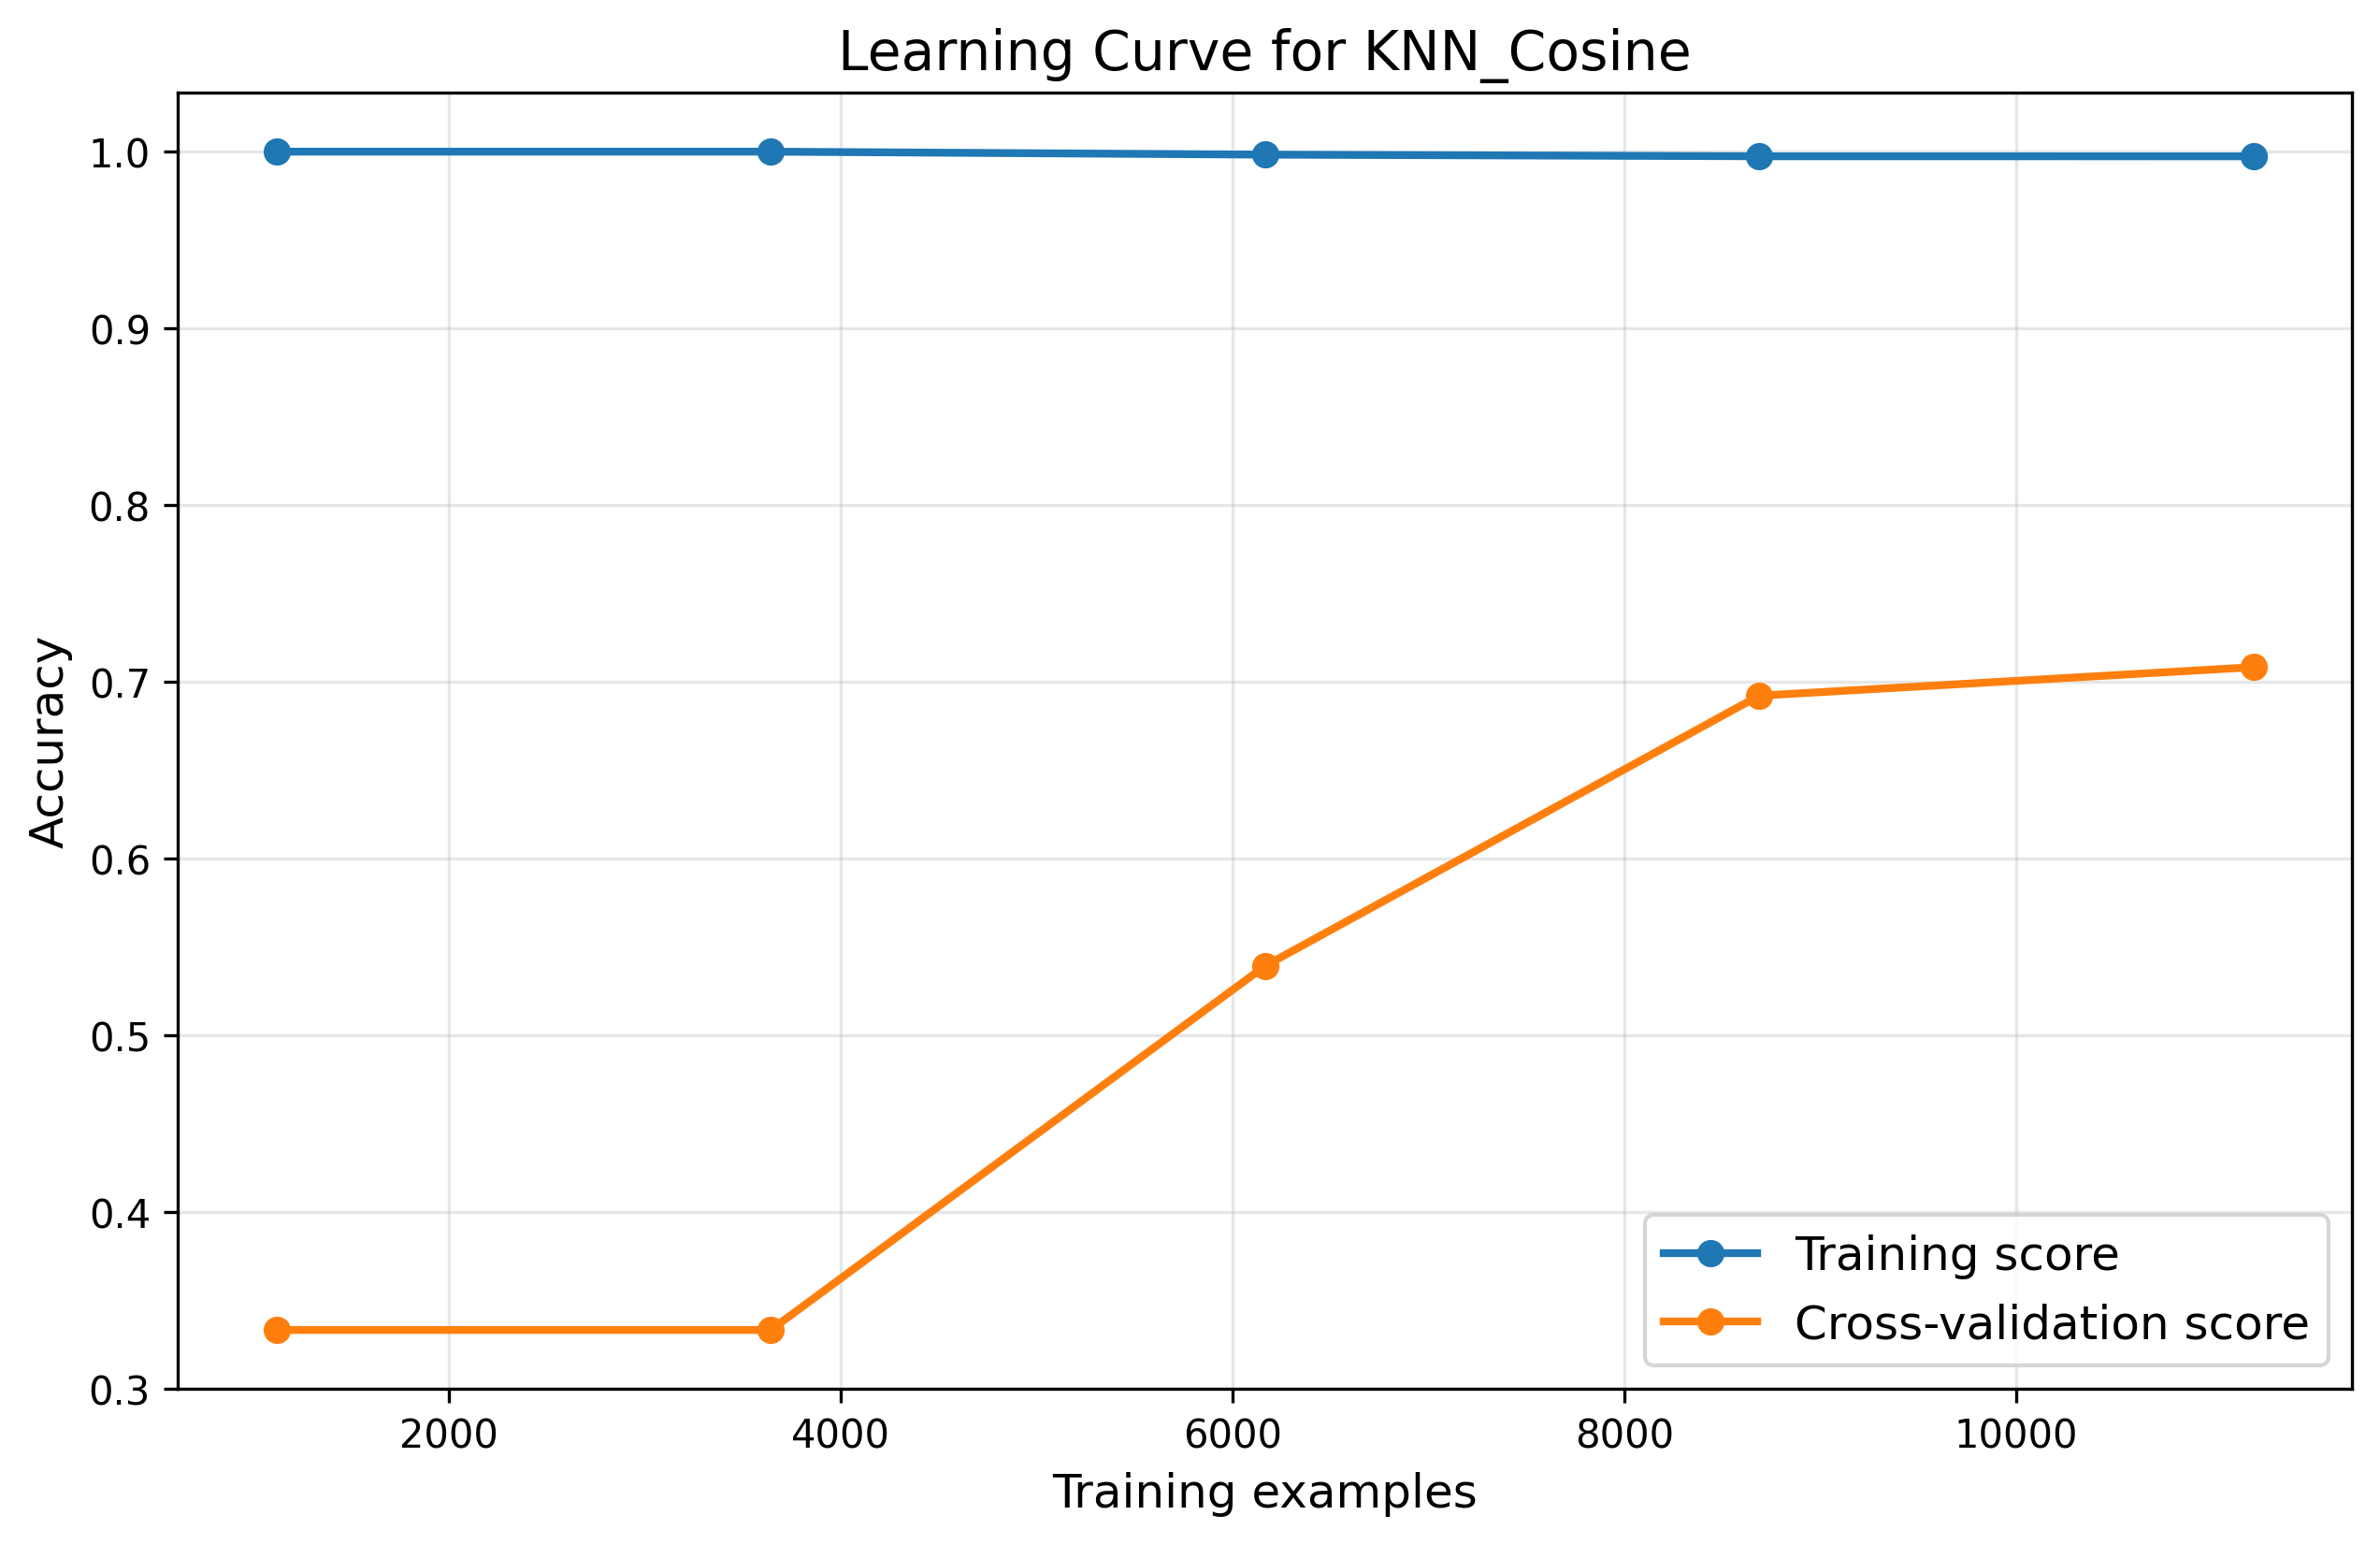
\includegraphics[width=\textwidth]{code/ResultsMainAugZip/plots/Block3_Probabilistic_Experiment_I/learning_curve_KNN_Cosine.png}
            \captionof{figure}{Learning Curve}
        \end{column}
        \begin{column}{0.33\textwidth}
            \centering
            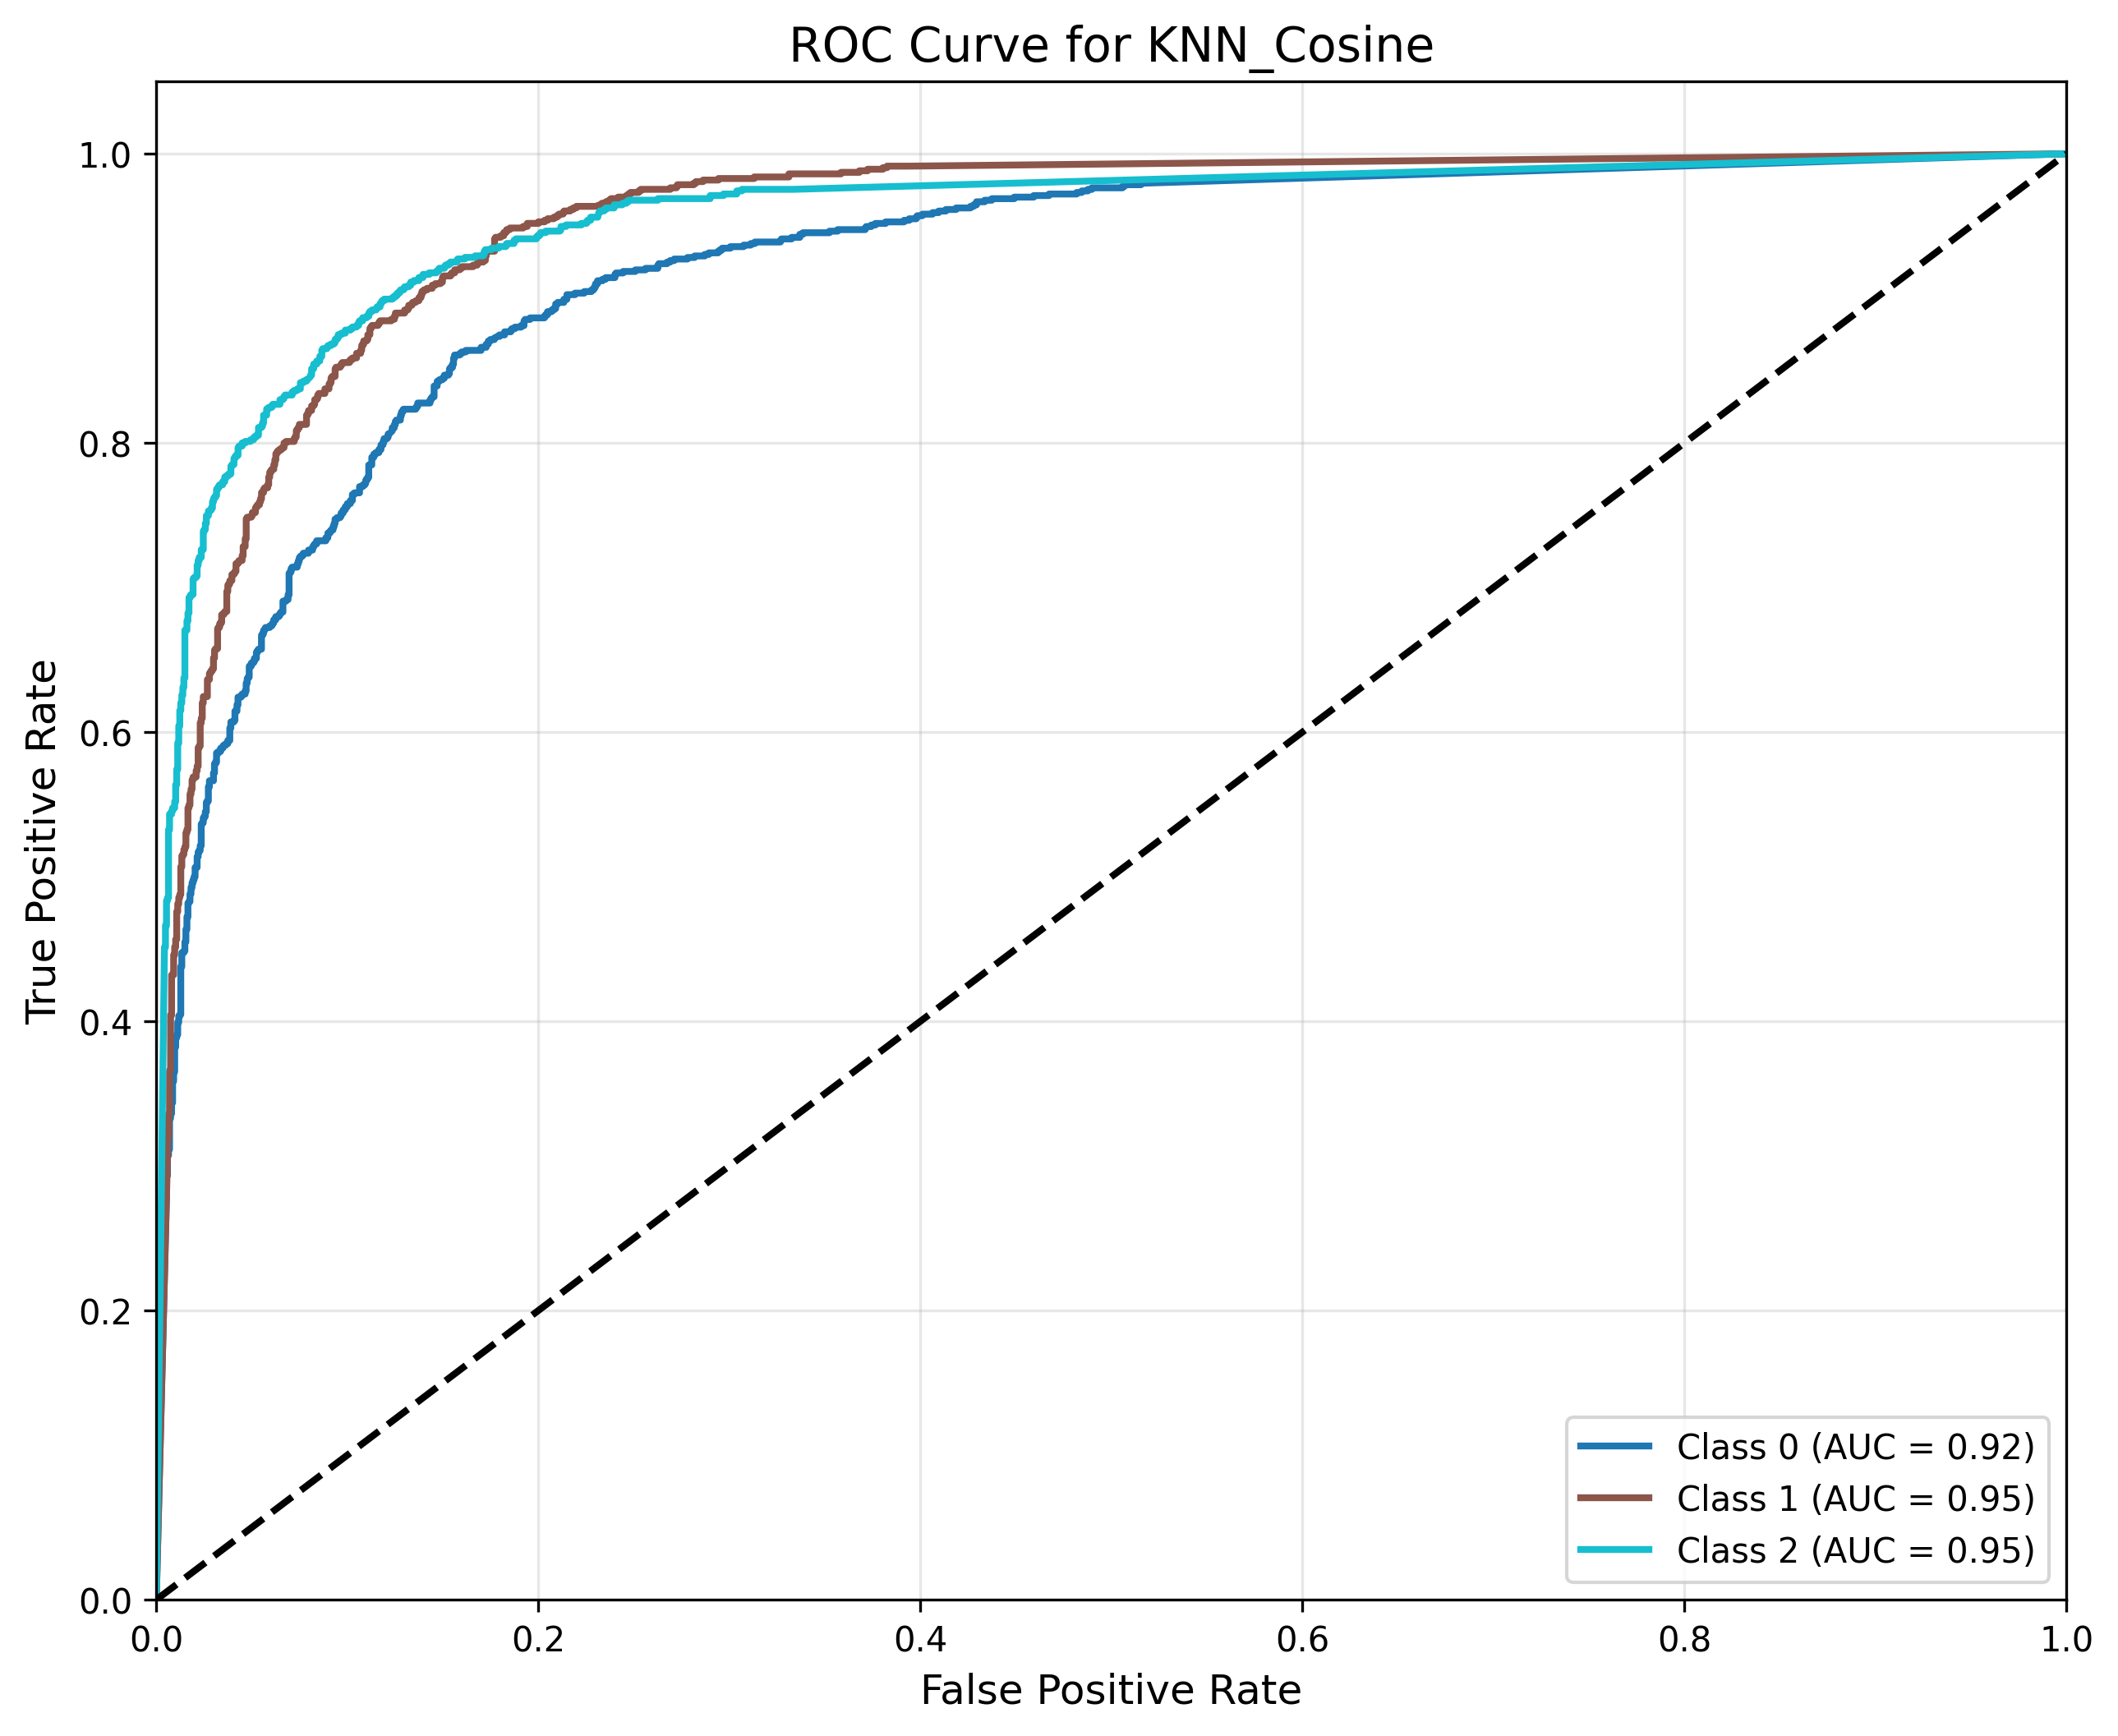
\includegraphics[width=\textwidth]{code/ResultsMainAugZip/plots/Block3_Probabilistic_Experiment_I/roc_curve_KNN_Cosine.png}
            \captionof{figure}{ROC Curve}
        \end{column}
    \end{columns}
    \end{frame}
    
    % Block 4: SVM Variants (Experiment I)
    \begin{frame}{Block 4: SVM Variants (Experiment I)}
    \framesubtitle{Best Model: Quadratic SVM}
    \begin{columns}
        \begin{column}{0.5\textwidth}
            \centering
            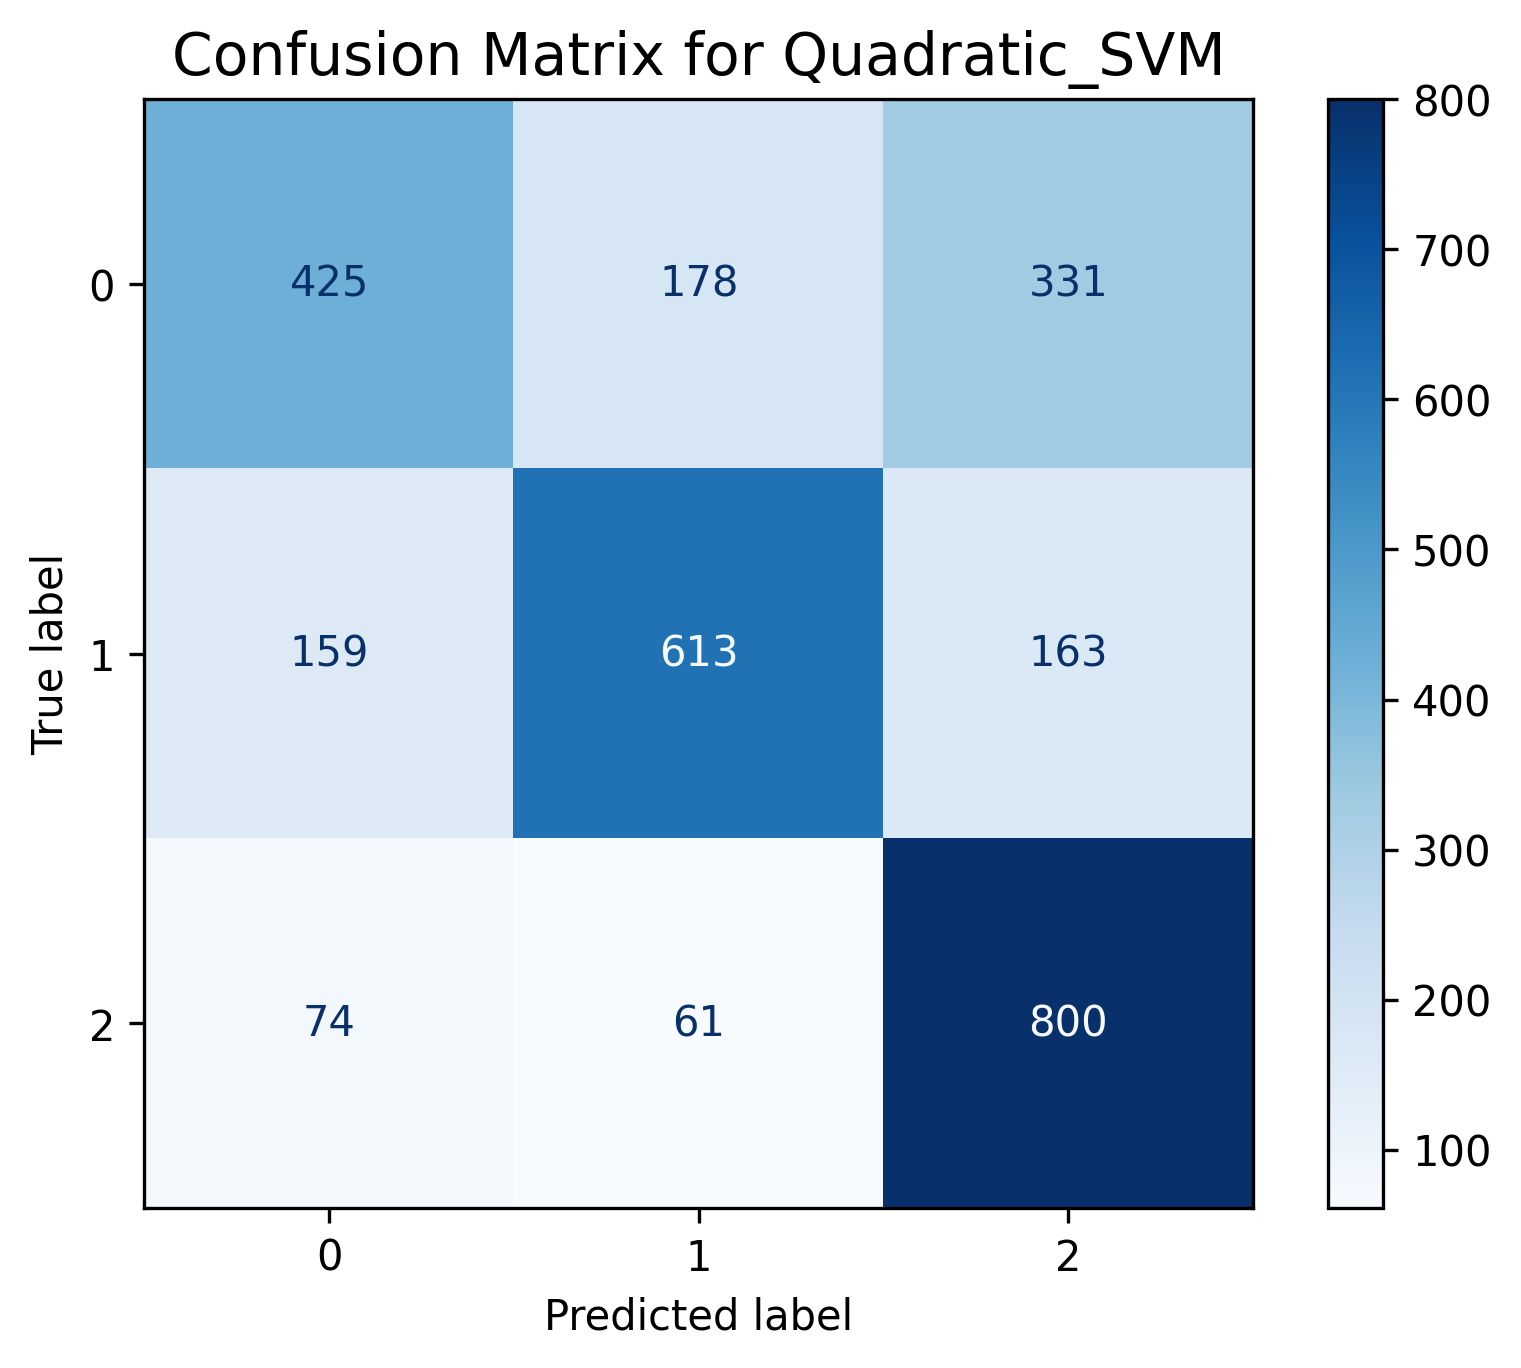
\includegraphics[width=0.9\textwidth]{code/ResultsMainAugZip/plots/Block4_SVM_Variants_Experiment_I/confusion_matrix_Quadratic_SVM.png}
            \captionof{figure}{Confusion Matrix}
        \end{column}
        \begin{column}{0.5\textwidth}
            \centering
            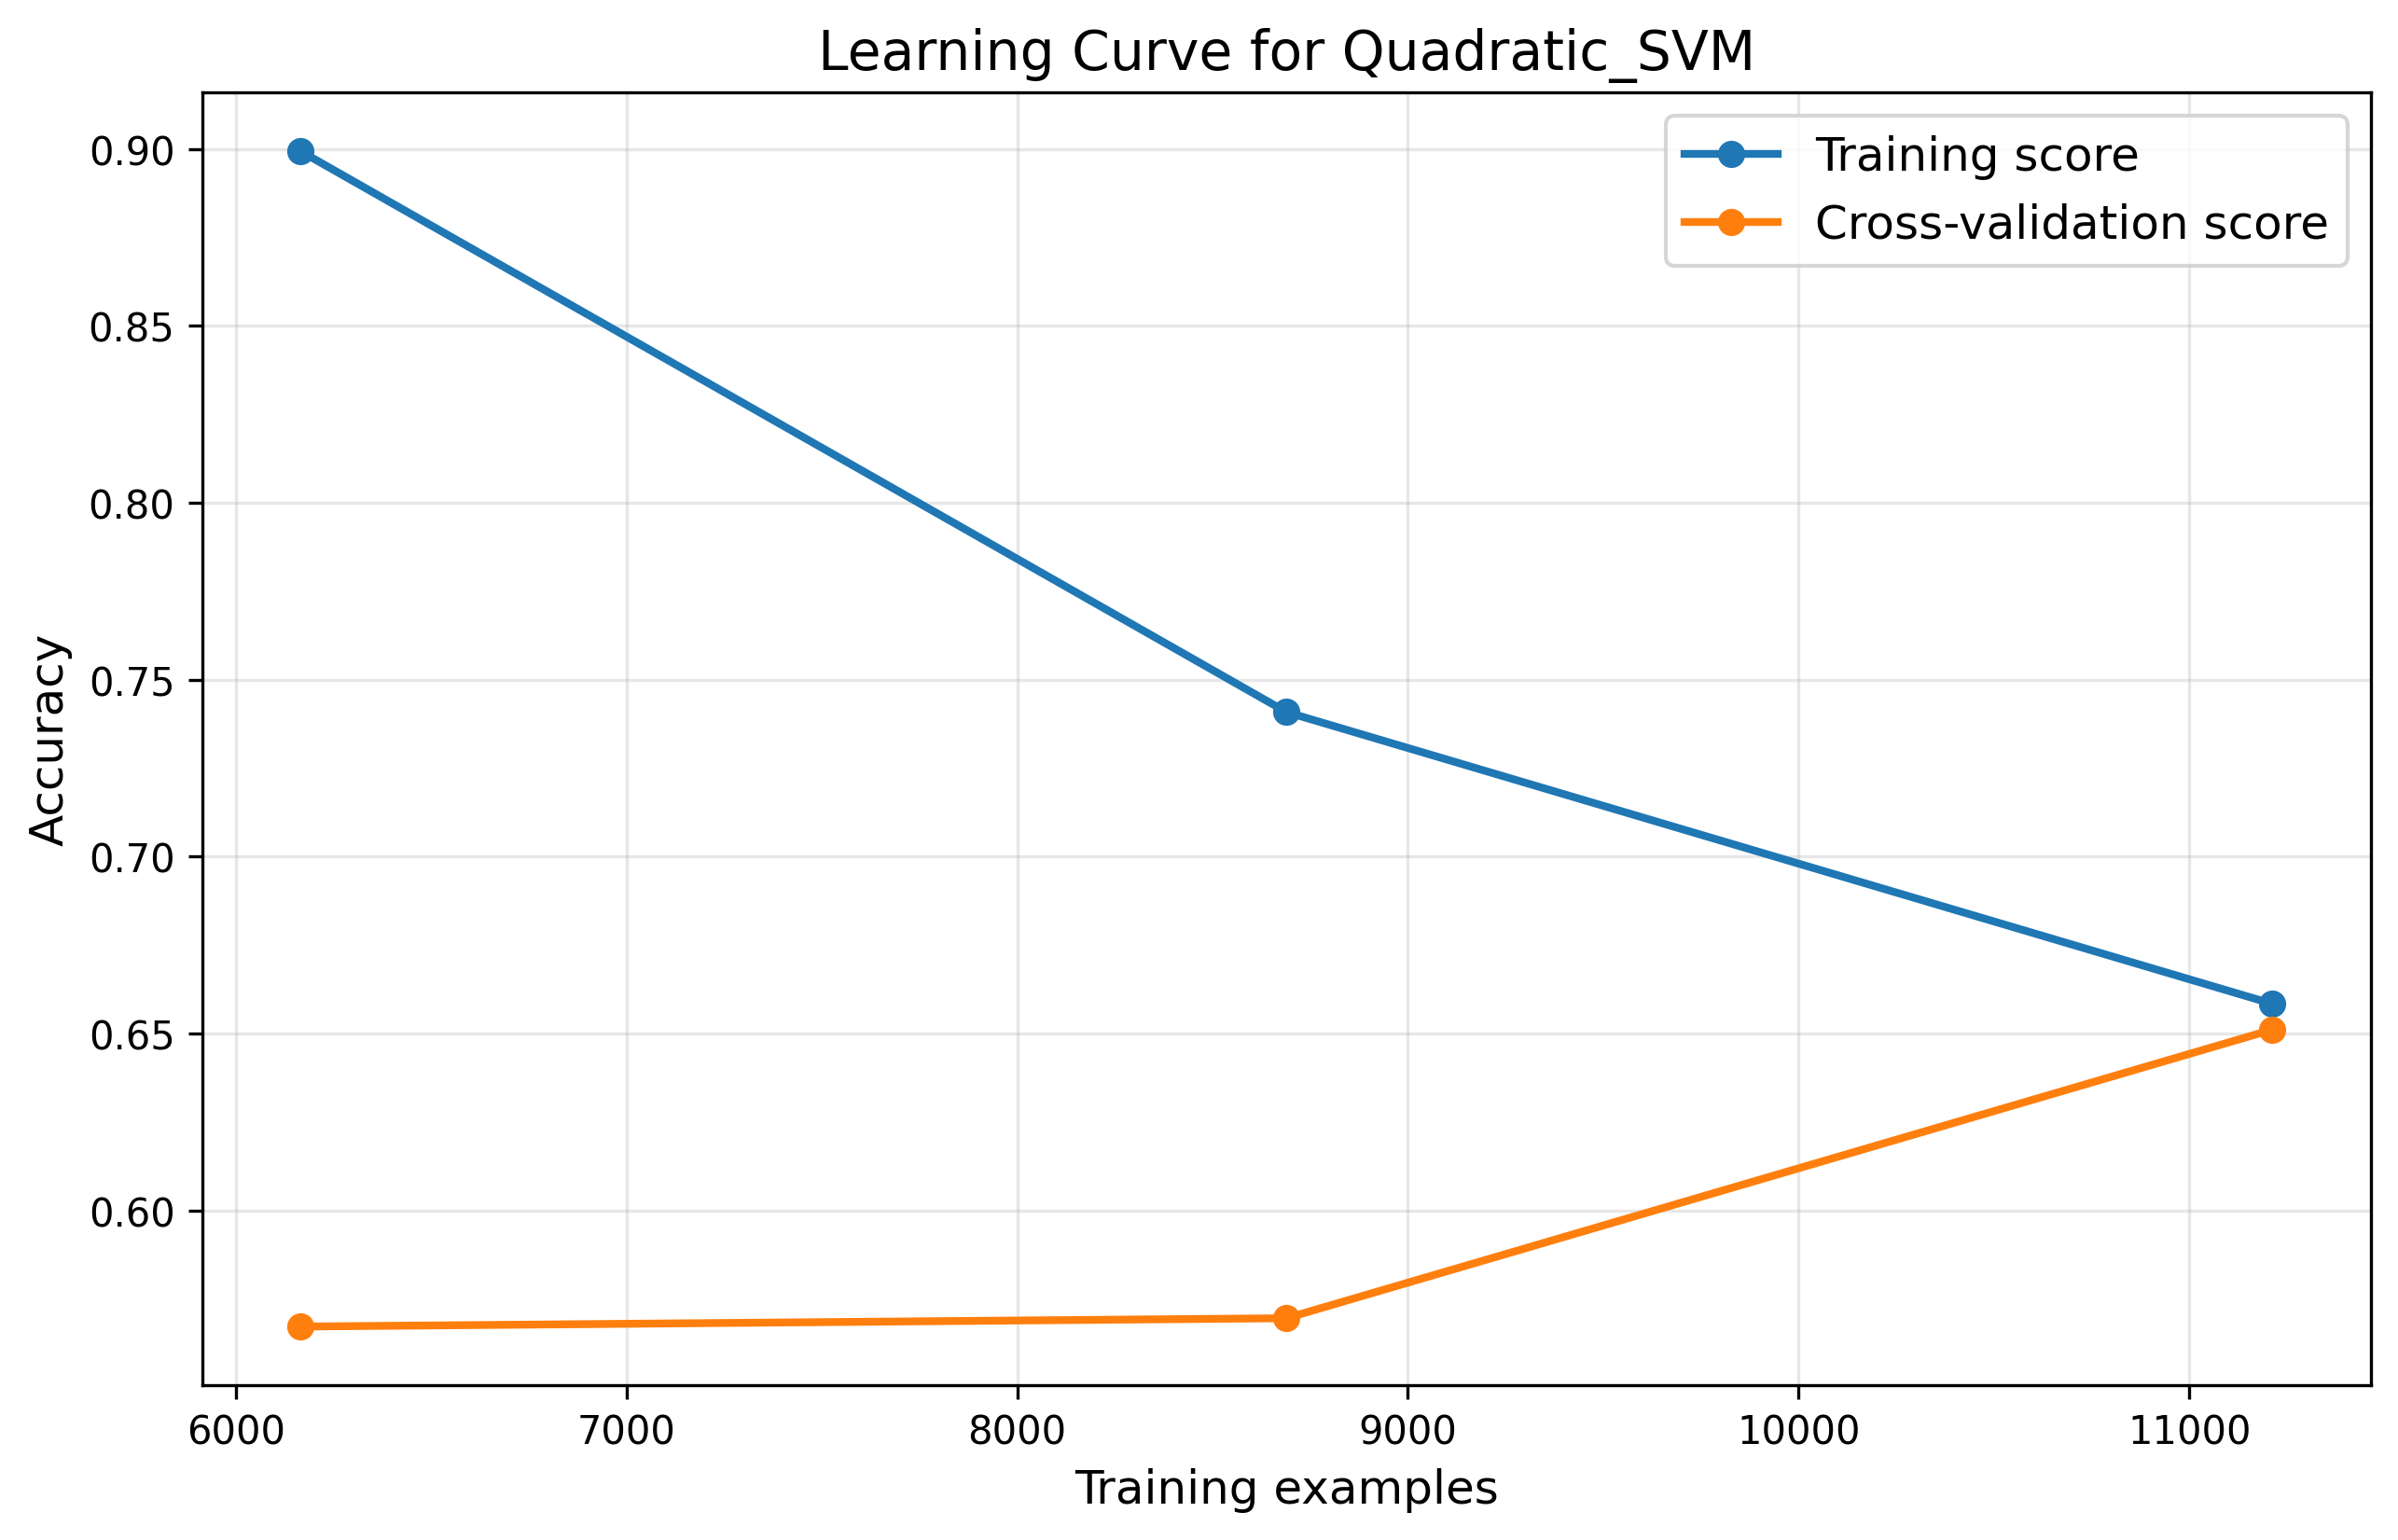
\includegraphics[width=0.9\textwidth]{code/ResultsMainAugZip/plots/Block4_SVM_Variants_Experiment_I/learning_curve_Quadratic_SVM.png}
            \captionof{figure}{Learning Curve}
        \end{column}
    \end{columns}
    \end{frame}
    
    % ==================== EXPERIMENT II PLOTS ====================
    % Block 1: Tree-Based (Experiment II)
    \begin{frame}{Block 1: Tree-Based Classifiers (Experiment II)}
    \framesubtitle{Best Model: Random Forest}
    \begin{columns}
        \begin{column}{0.33\textwidth}
            \centering
            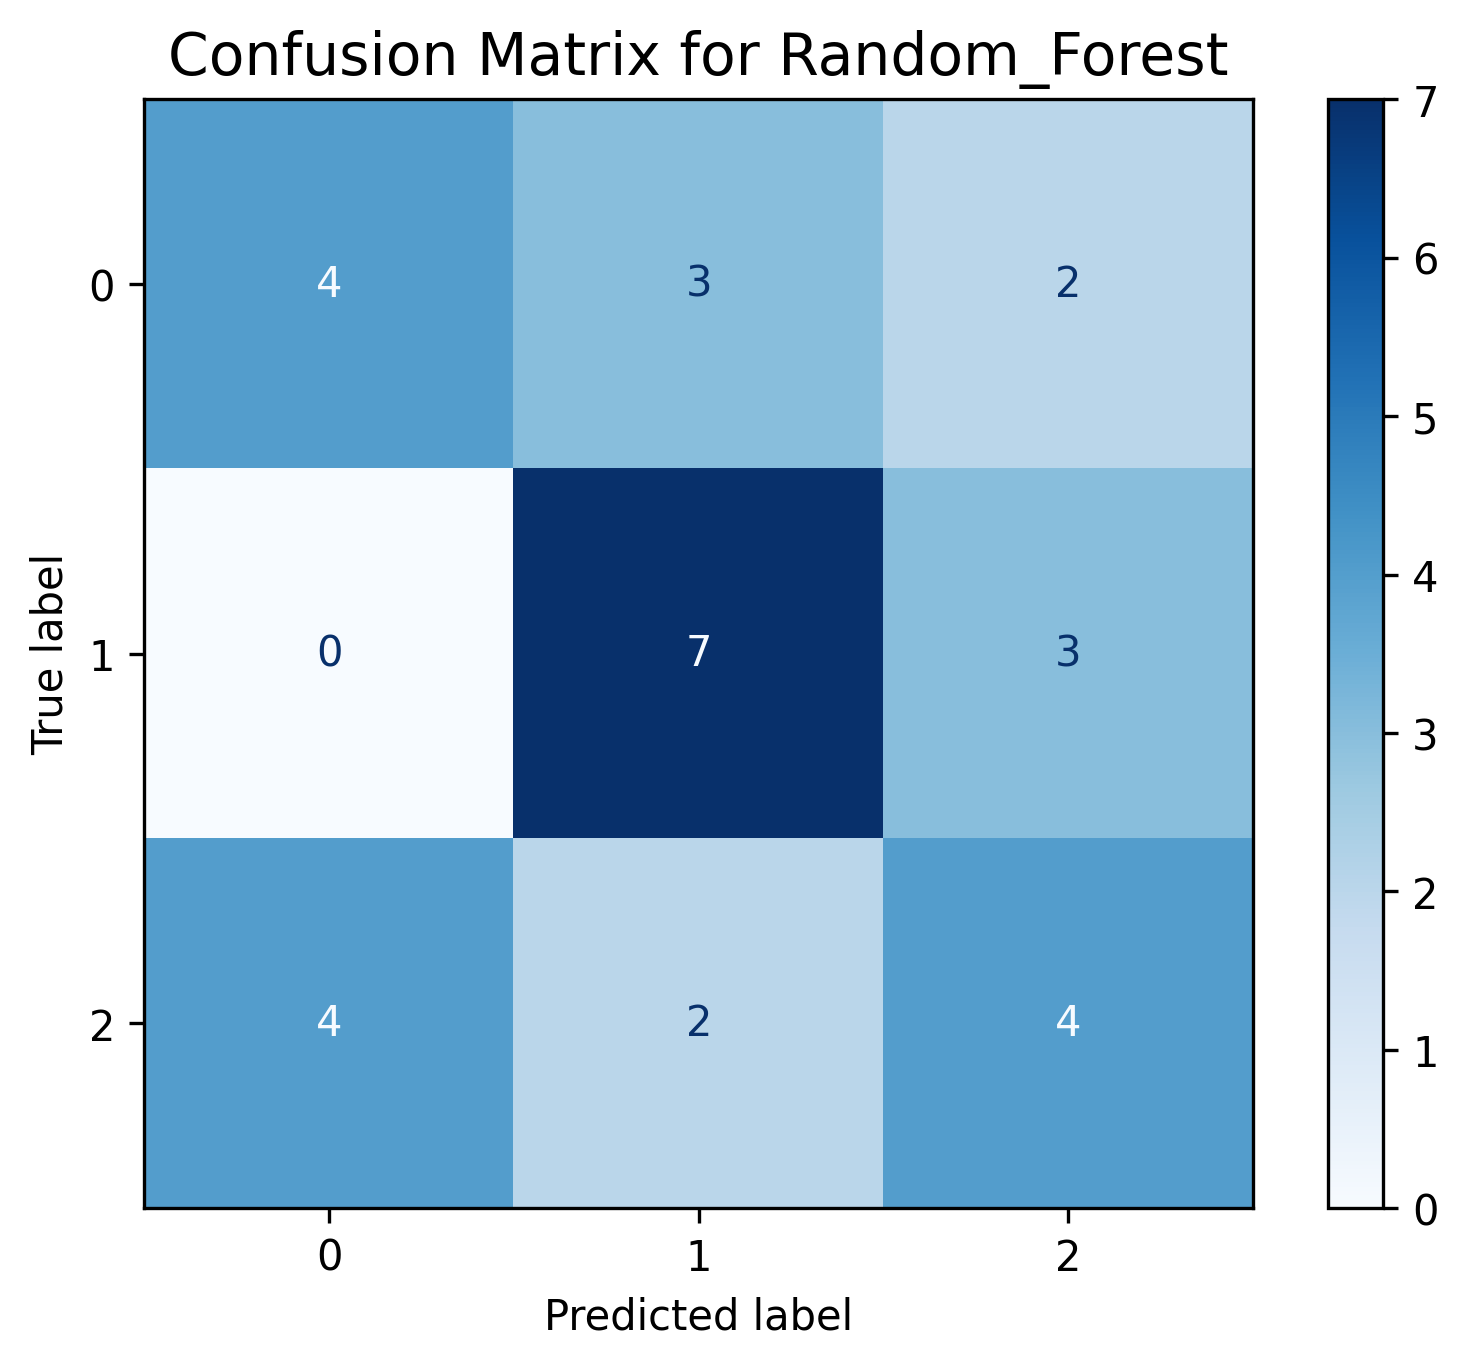
\includegraphics[width=\textwidth]{code/ResultsMainAugZip/plots/Block1_Tree_Based_Experiment_II/confusion_matrix_Random_Forest.png}
            \captionof{figure}{Confusion Matrix}
        \end{column}
        \begin{column}{0.33\textwidth}
            \centering
            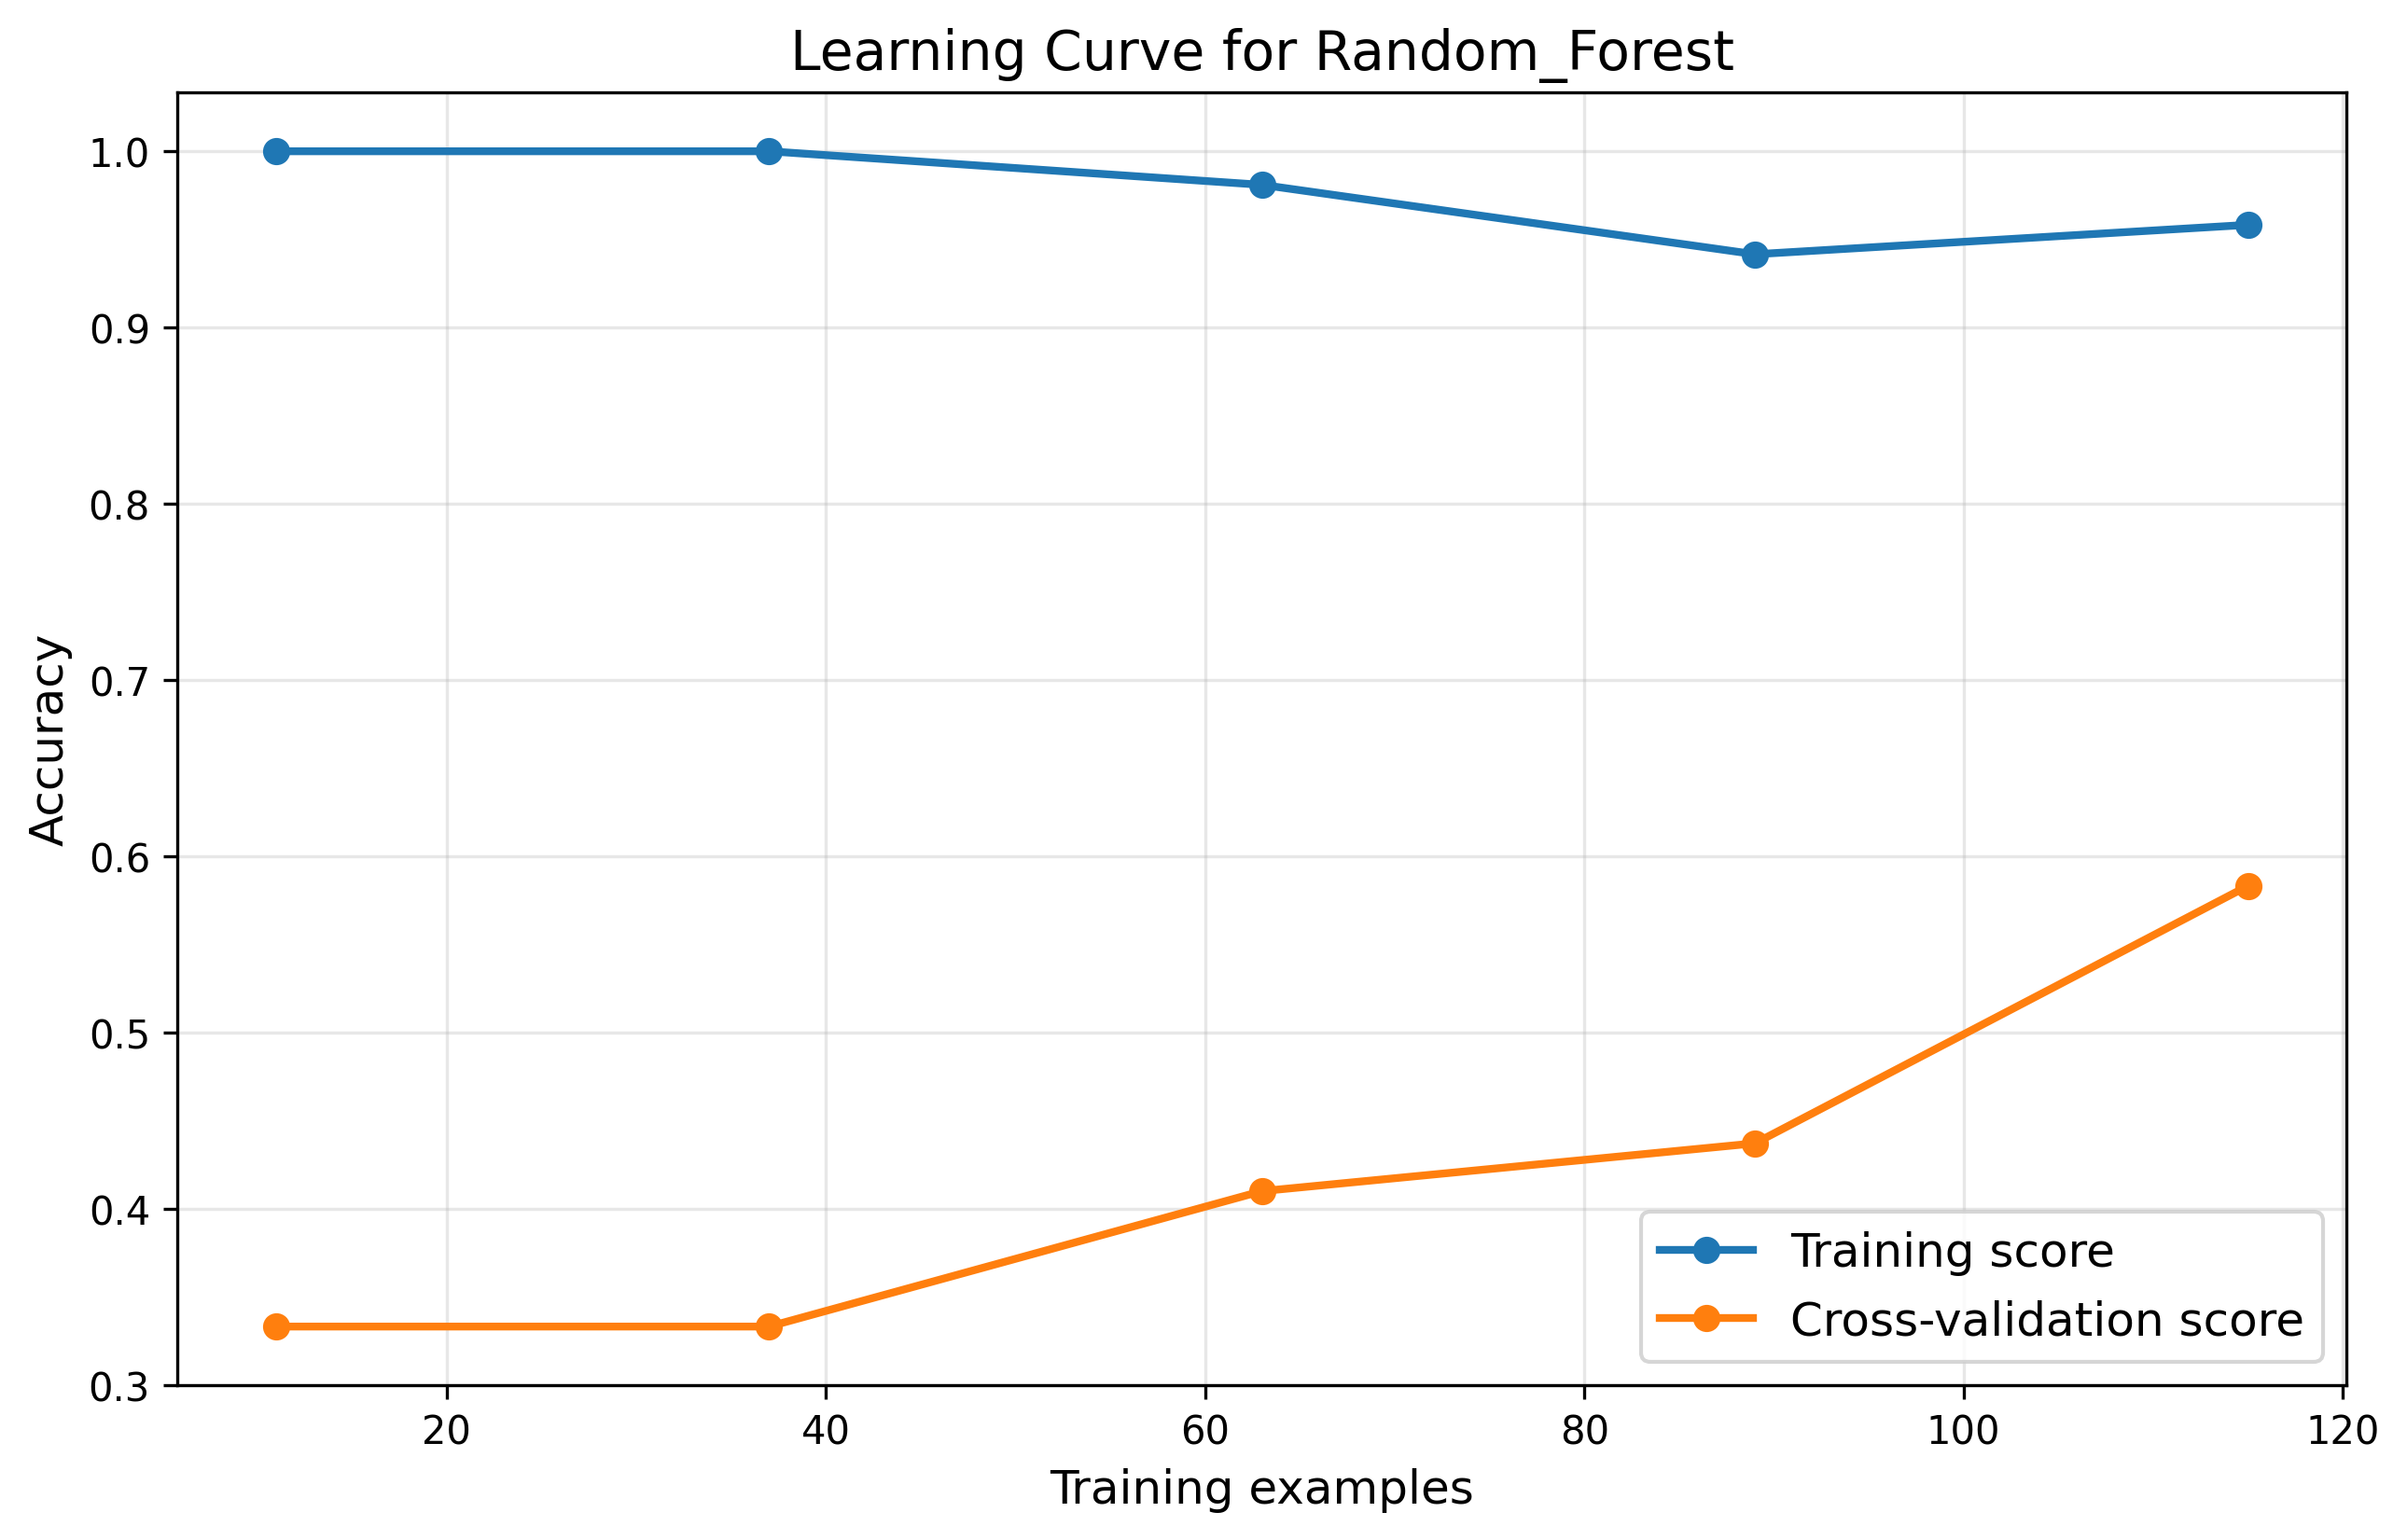
\includegraphics[width=\textwidth]{code/ResultsMainAugZip/plots/Block1_Tree_Based_Experiment_II/learning_curve_Random_Forest.png}
            \captionof{figure}{Learning Curve}
        \end{column}
        \begin{column}{0.33\textwidth}
            \centering
            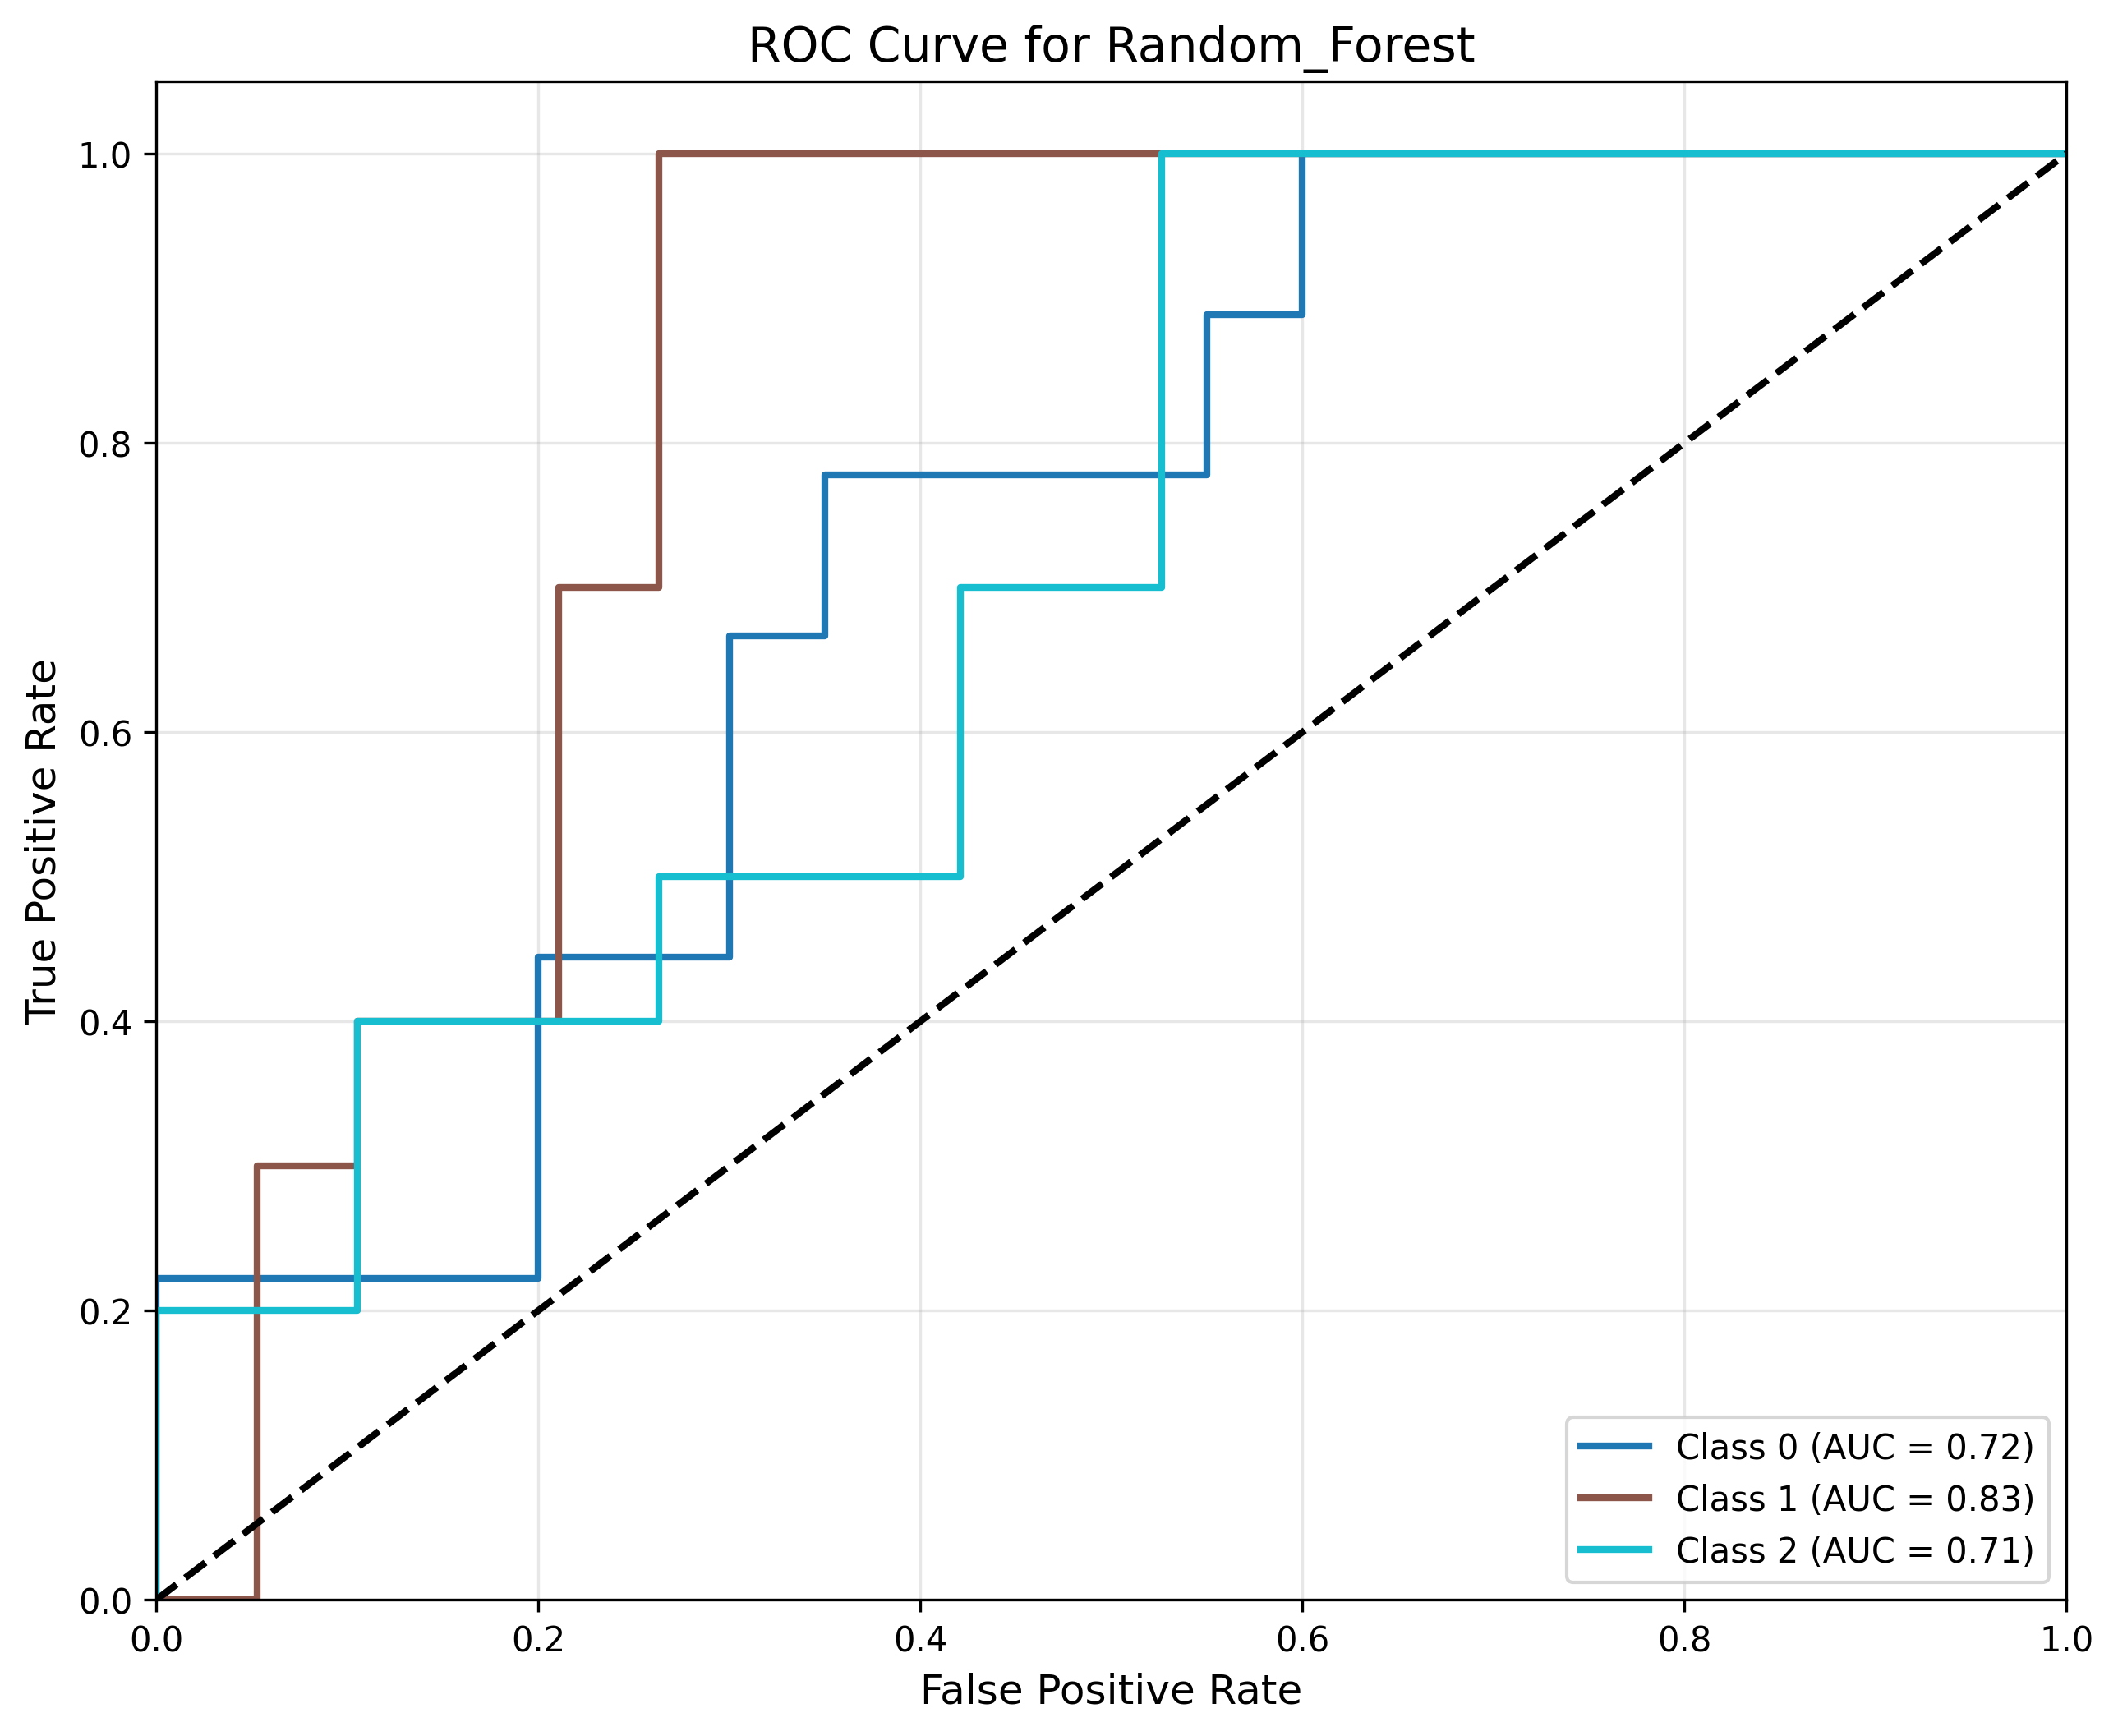
\includegraphics[width=\textwidth]{code/ResultsMainAugZip/plots/Block1_Tree_Based_Experiment_II/roc_curve_Random_Forest.png}
            \captionof{figure}{ROC Curve}
        \end{column}
    \end{columns}
    \end{frame}
    
    % Block 2: KNN Variants (Experiment II)
    \begin{frame}{Block 2: KNN Variants (Experiment II)}
    \framesubtitle{Best Model: KNN Fine}
    \begin{columns}
        \begin{column}{0.33\textwidth}
            \centering
            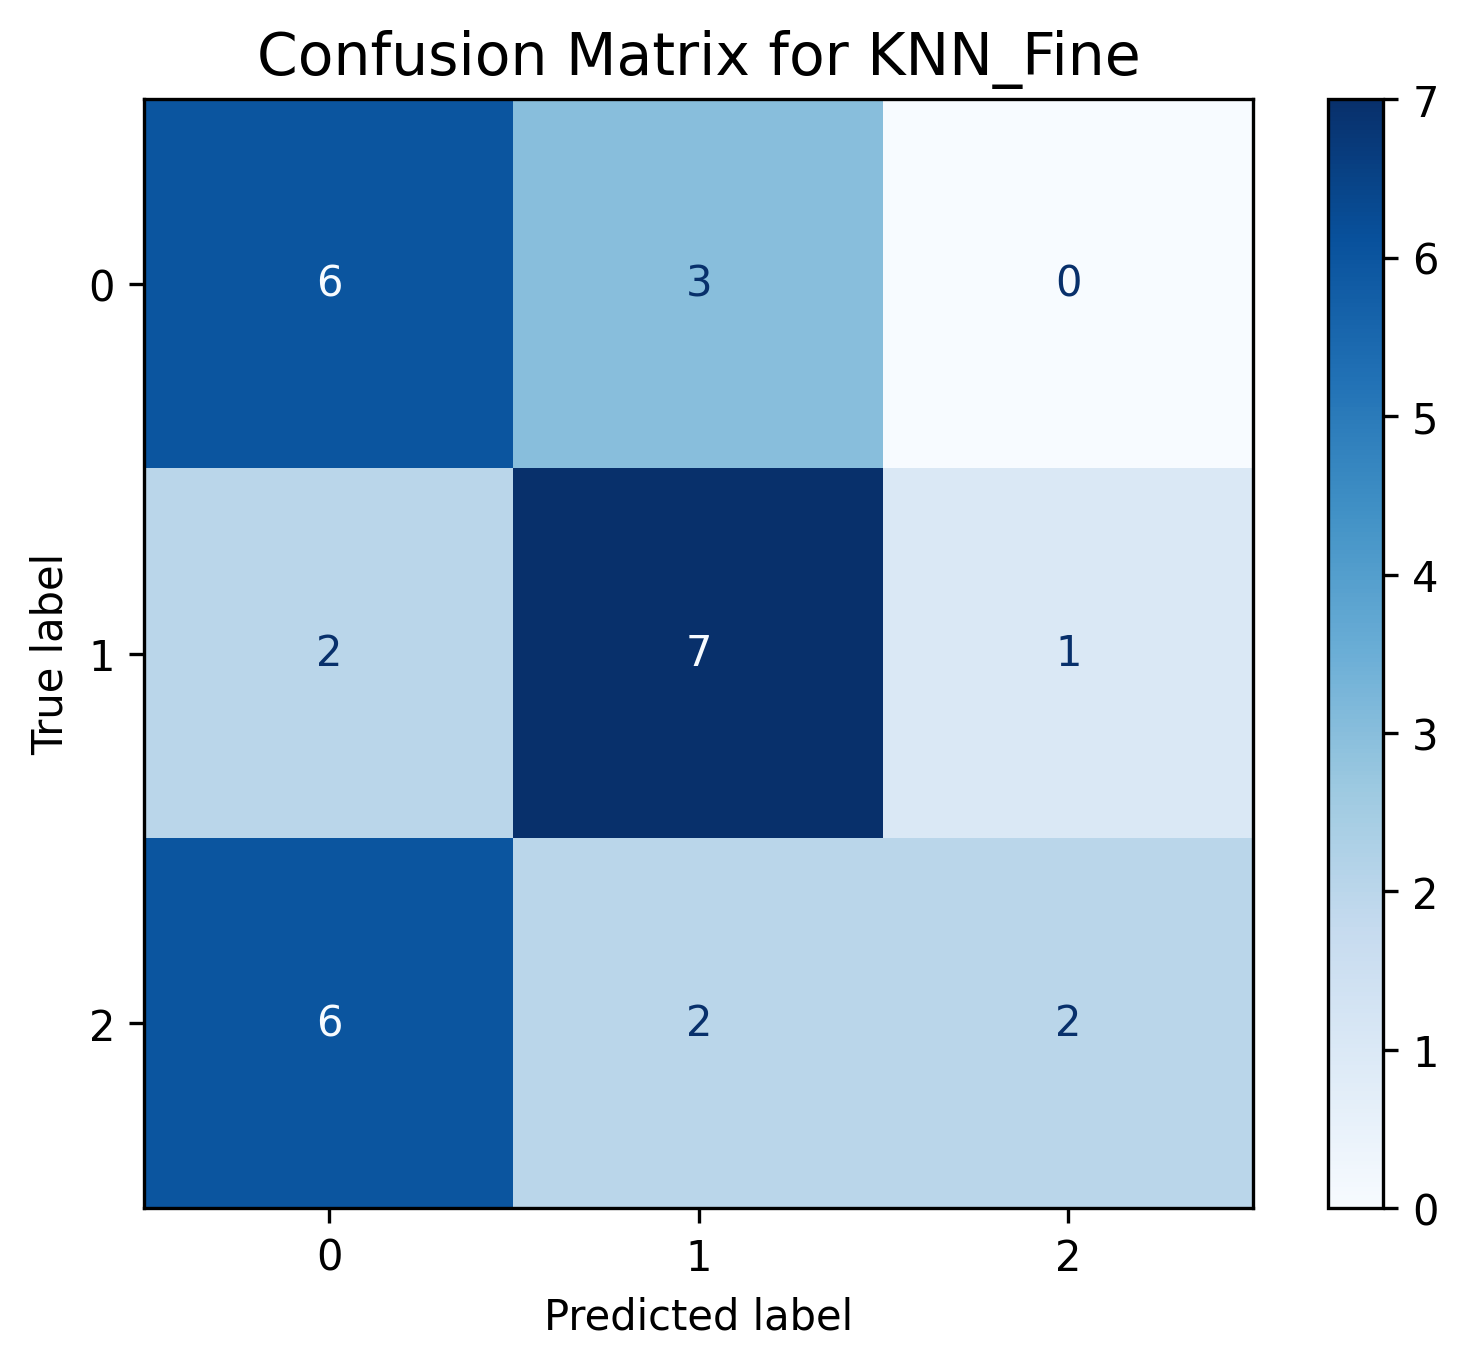
\includegraphics[width=\textwidth]{code/ResultsMainAugZip/plots/Block2_KNN_Variants_Experiment_II/confusion_matrix_KNN_Fine.png}
            \captionof{figure}{Confusion Matrix}
        \end{column}
        \begin{column}{0.33\textwidth}
            \centering
            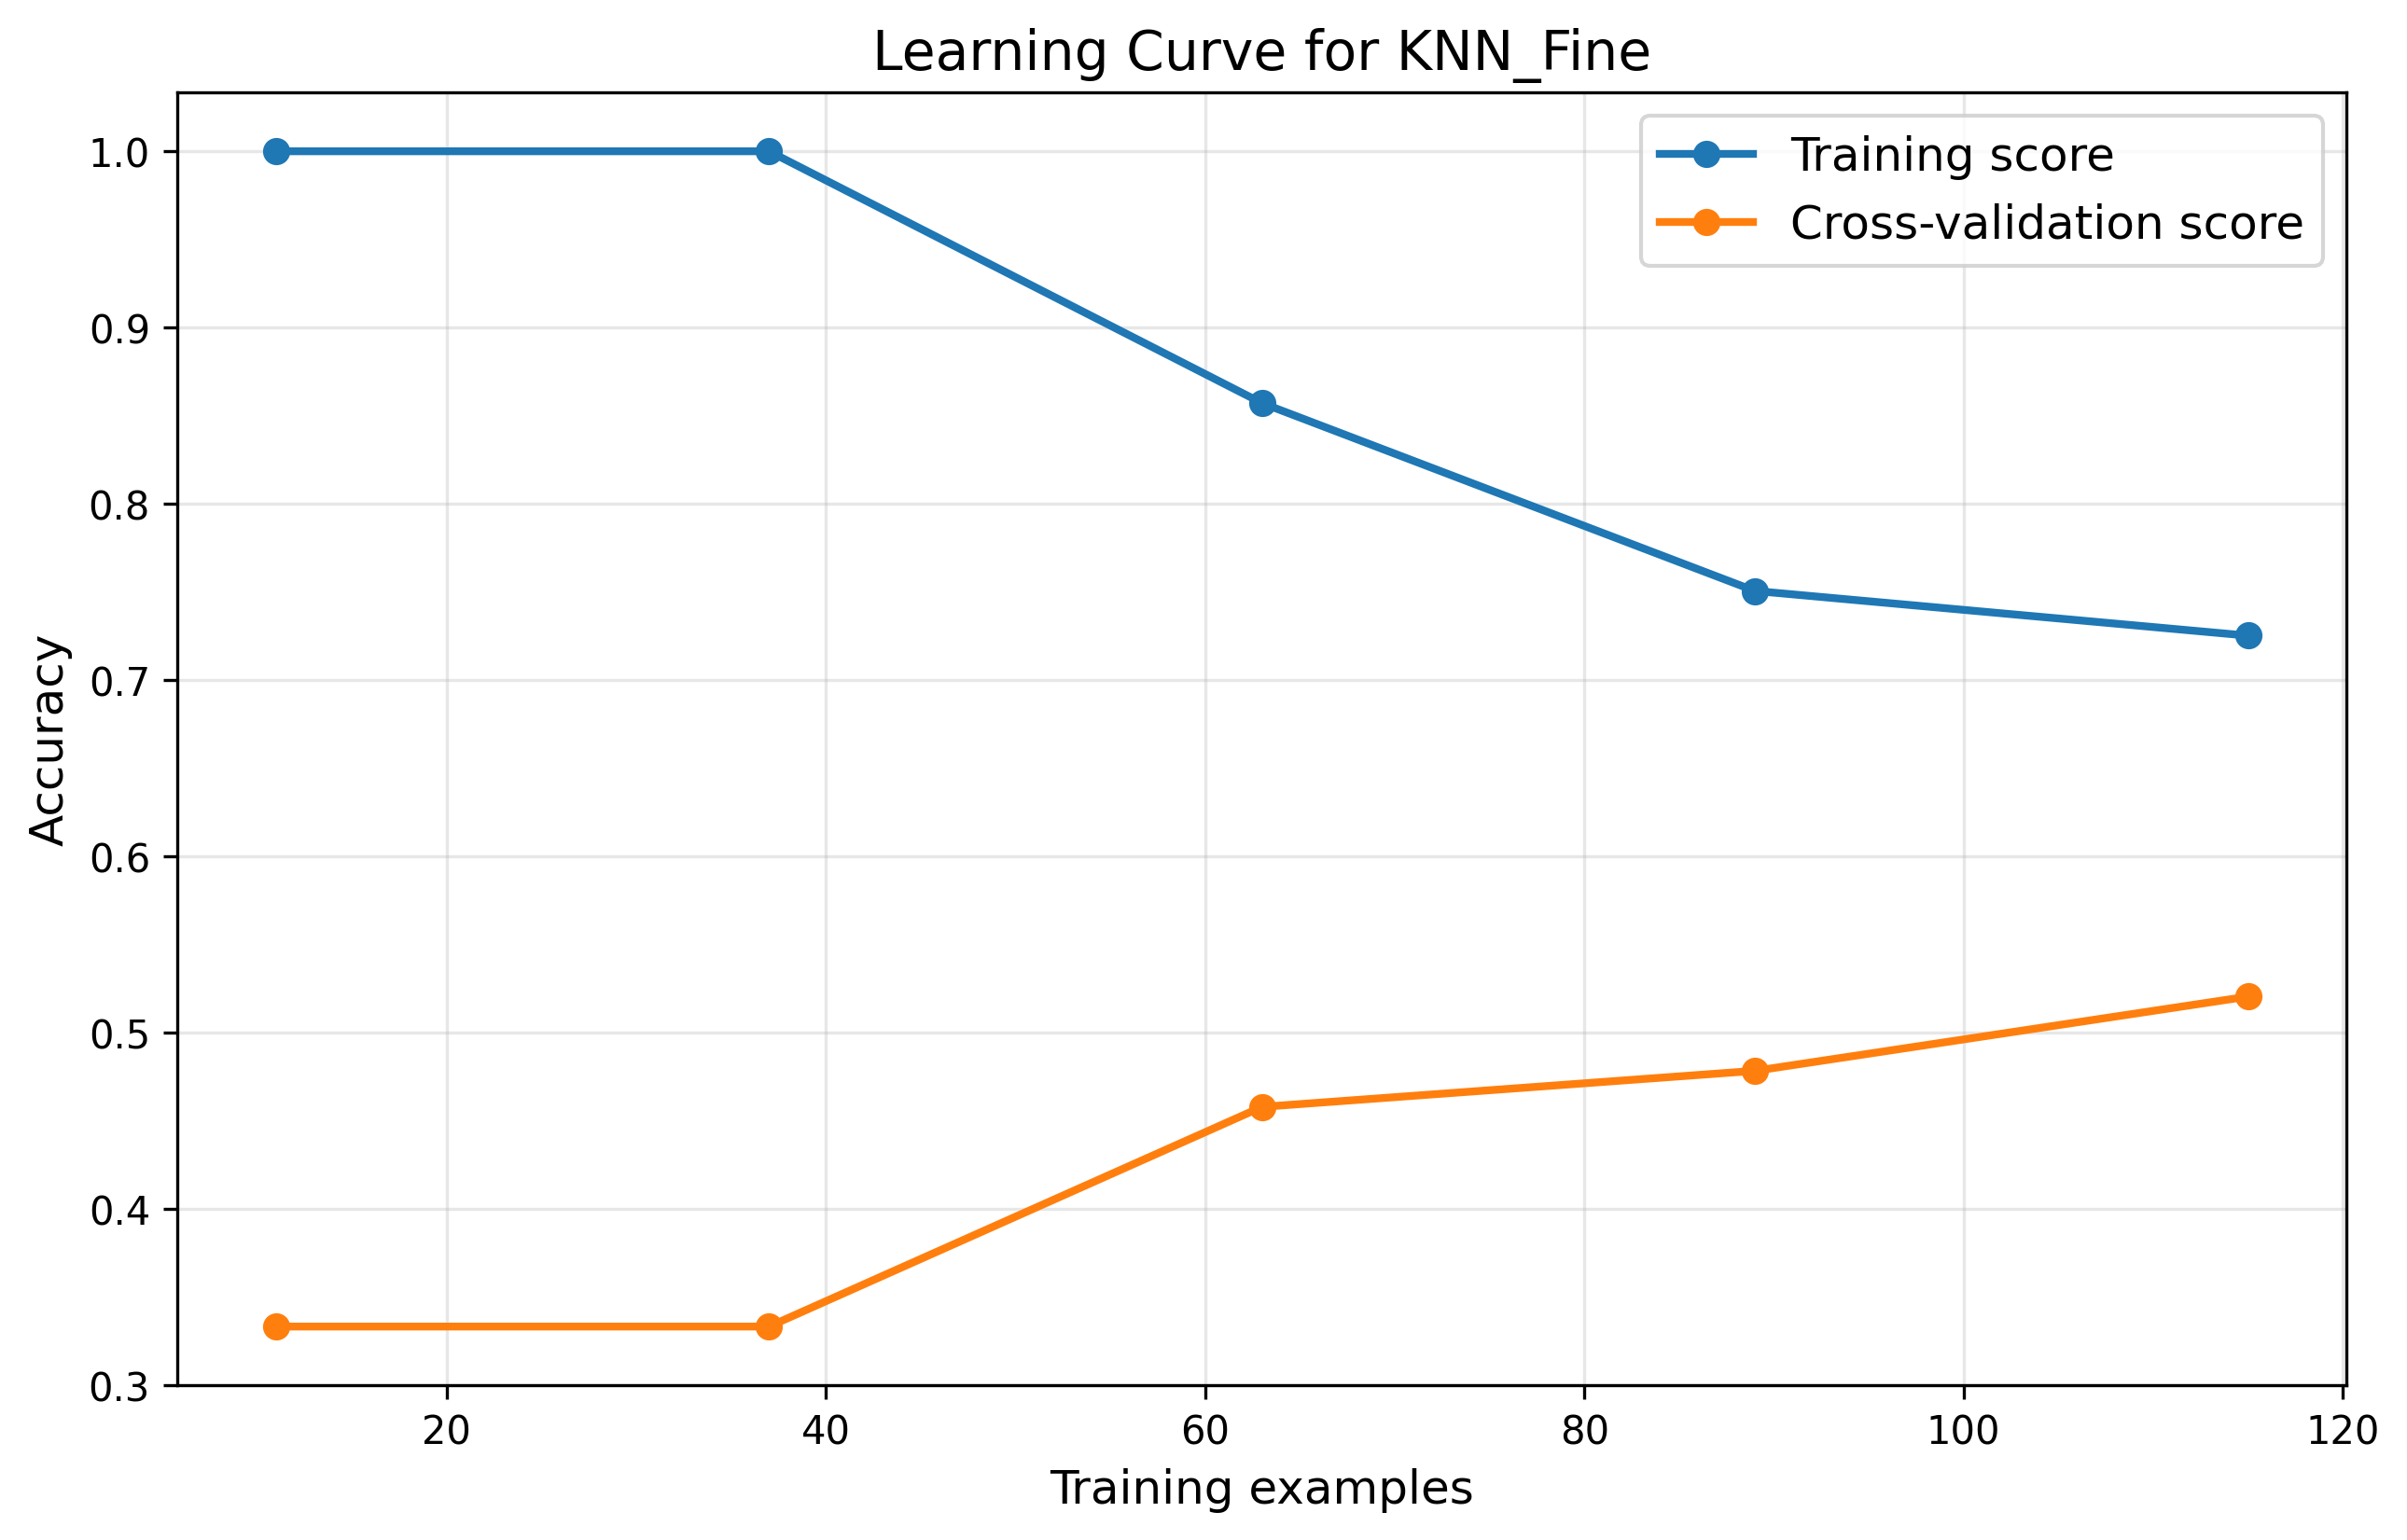
\includegraphics[width=\textwidth]{code/ResultsMainAugZip/plots/Block2_KNN_Variants_Experiment_II/learning_curve_KNN_Fine.png}
            \captionof{figure}{Learning Curve}
        \end{column}
        \begin{column}{0.33\textwidth}
            \centering
            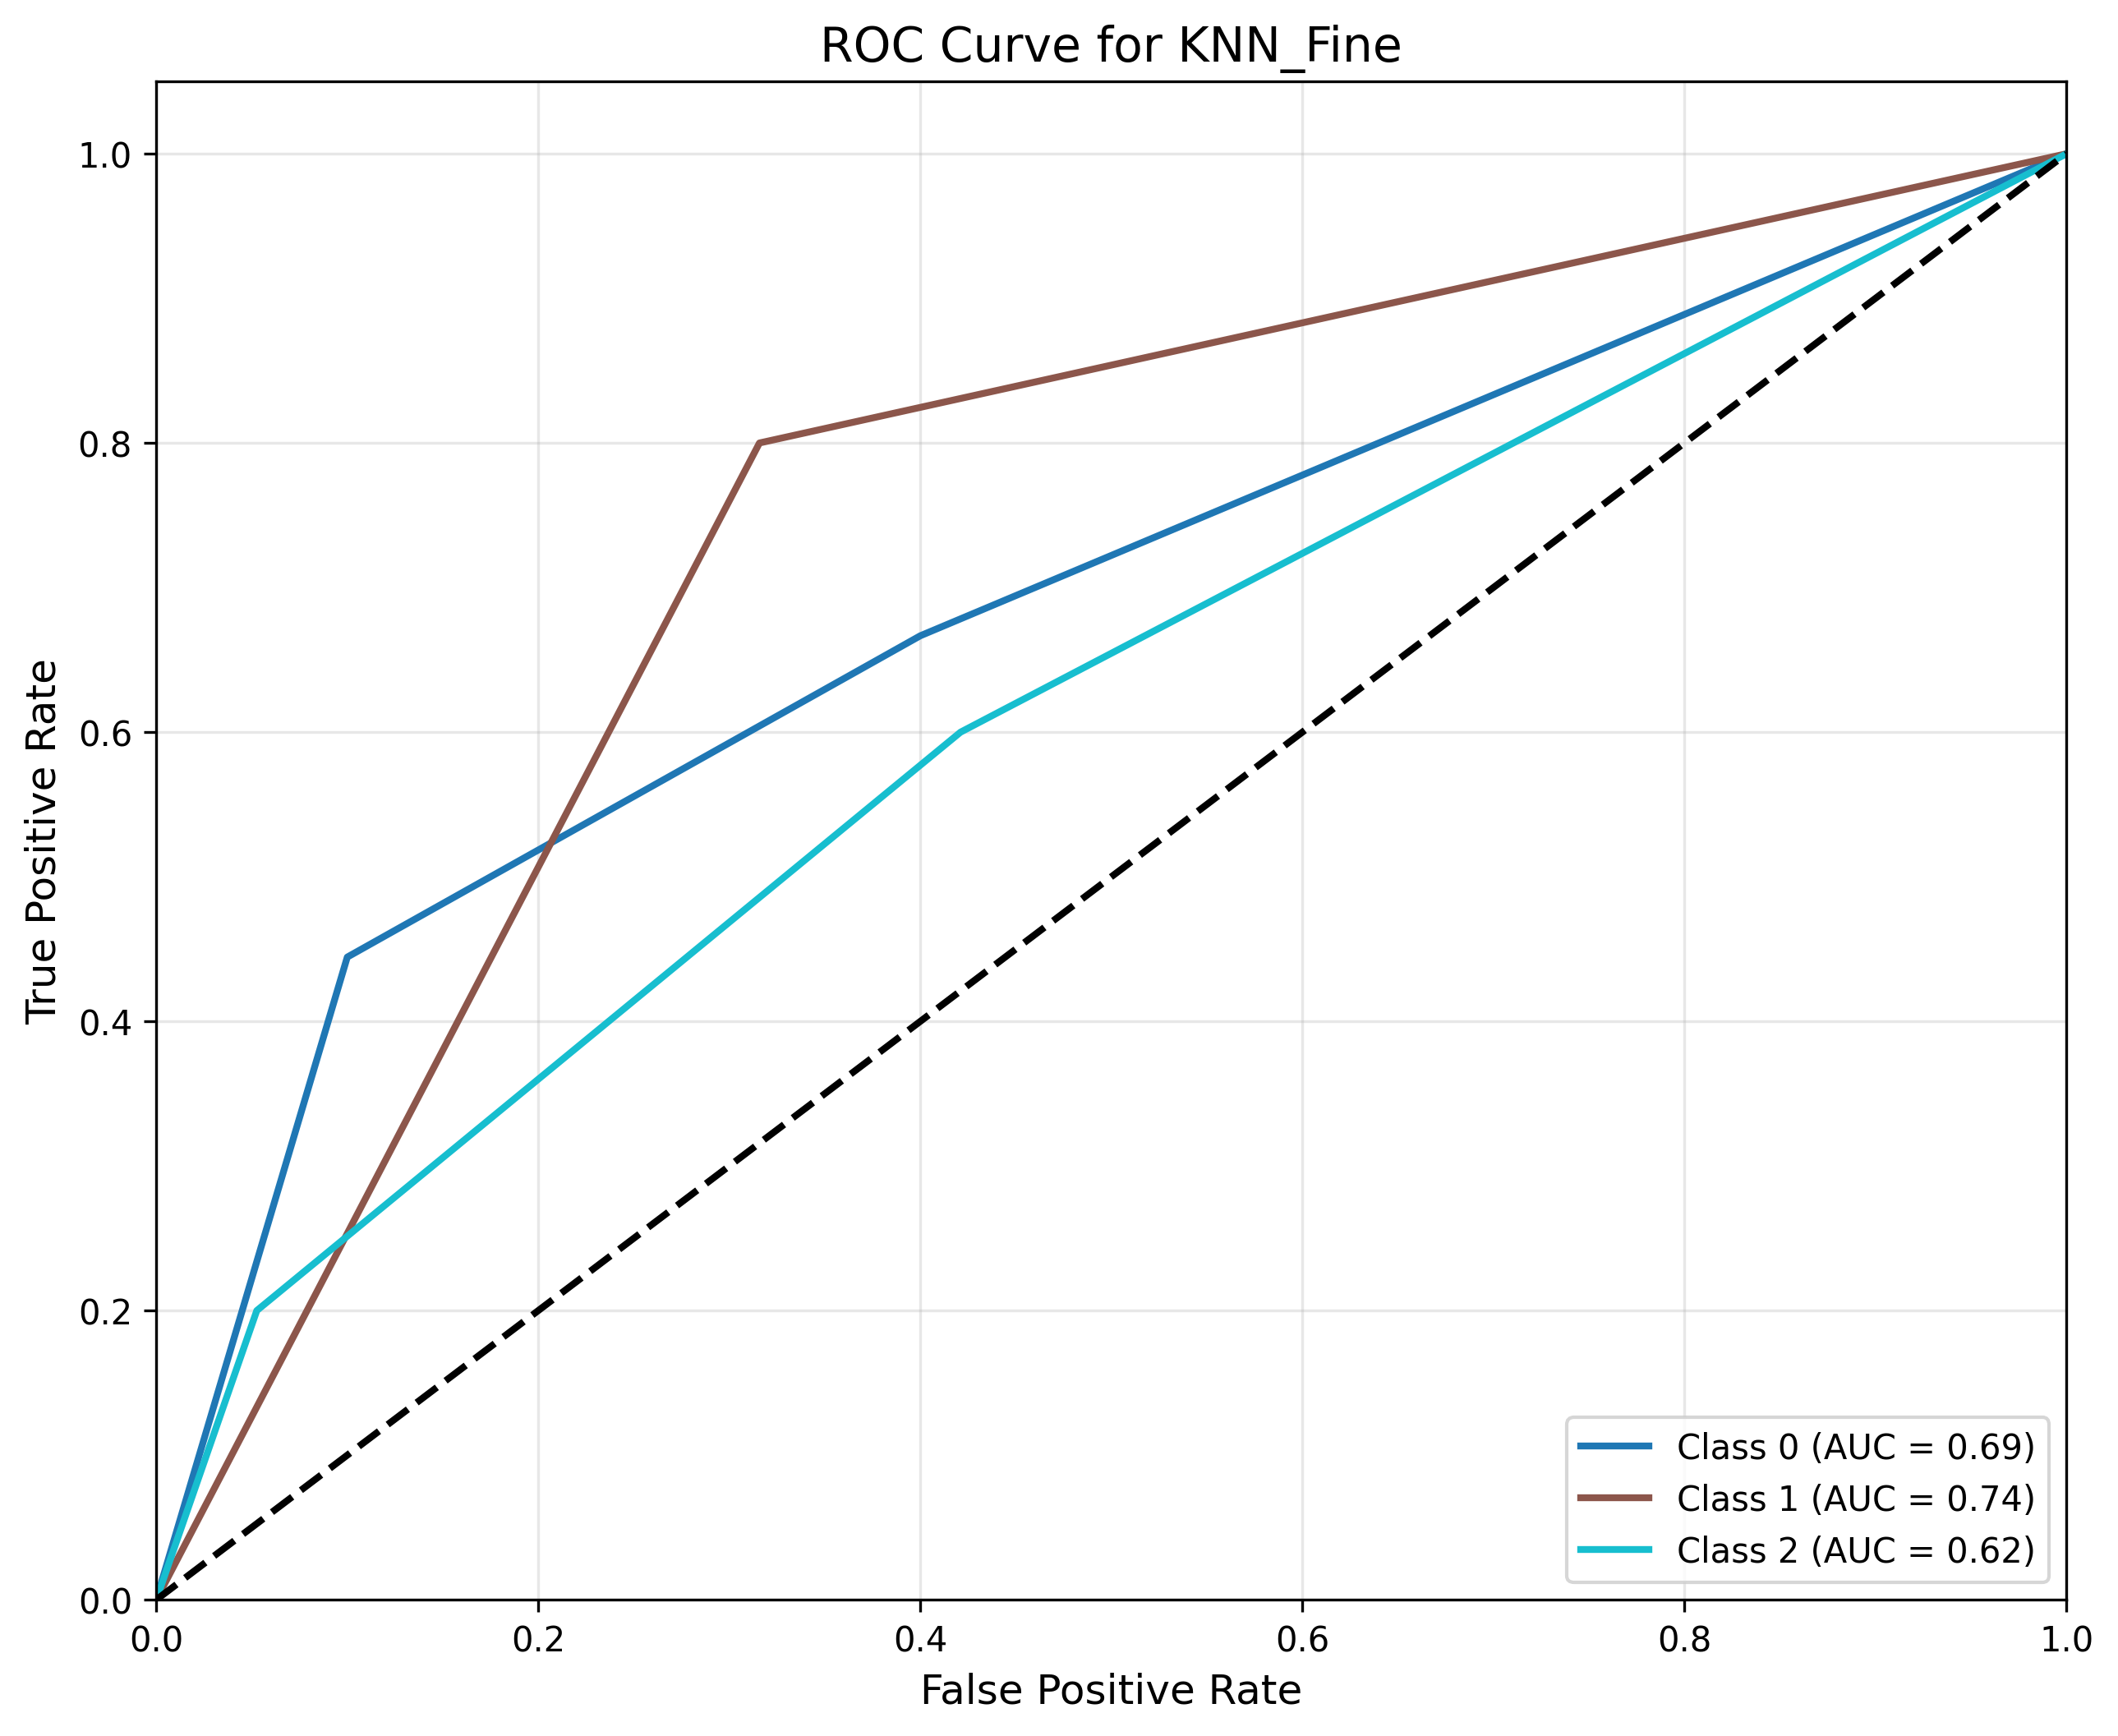
\includegraphics[width=\textwidth]{code/ResultsMainAugZip/plots/Block2_KNN_Variants_Experiment_II/roc_curve_KNN_Fine.png}
            \captionof{figure}{ROC Curve}
        \end{column}
    \end{columns}
    \end{frame}
    
    % Block 3: Probabilistic (Experiment II)
    \begin{frame}{Block 3: Probabilistic Classifiers (Experiment II)}
    \framesubtitle{Best Model: KNN Cosine}
    \begin{columns}
        \begin{column}{0.33\textwidth}
            \centering
            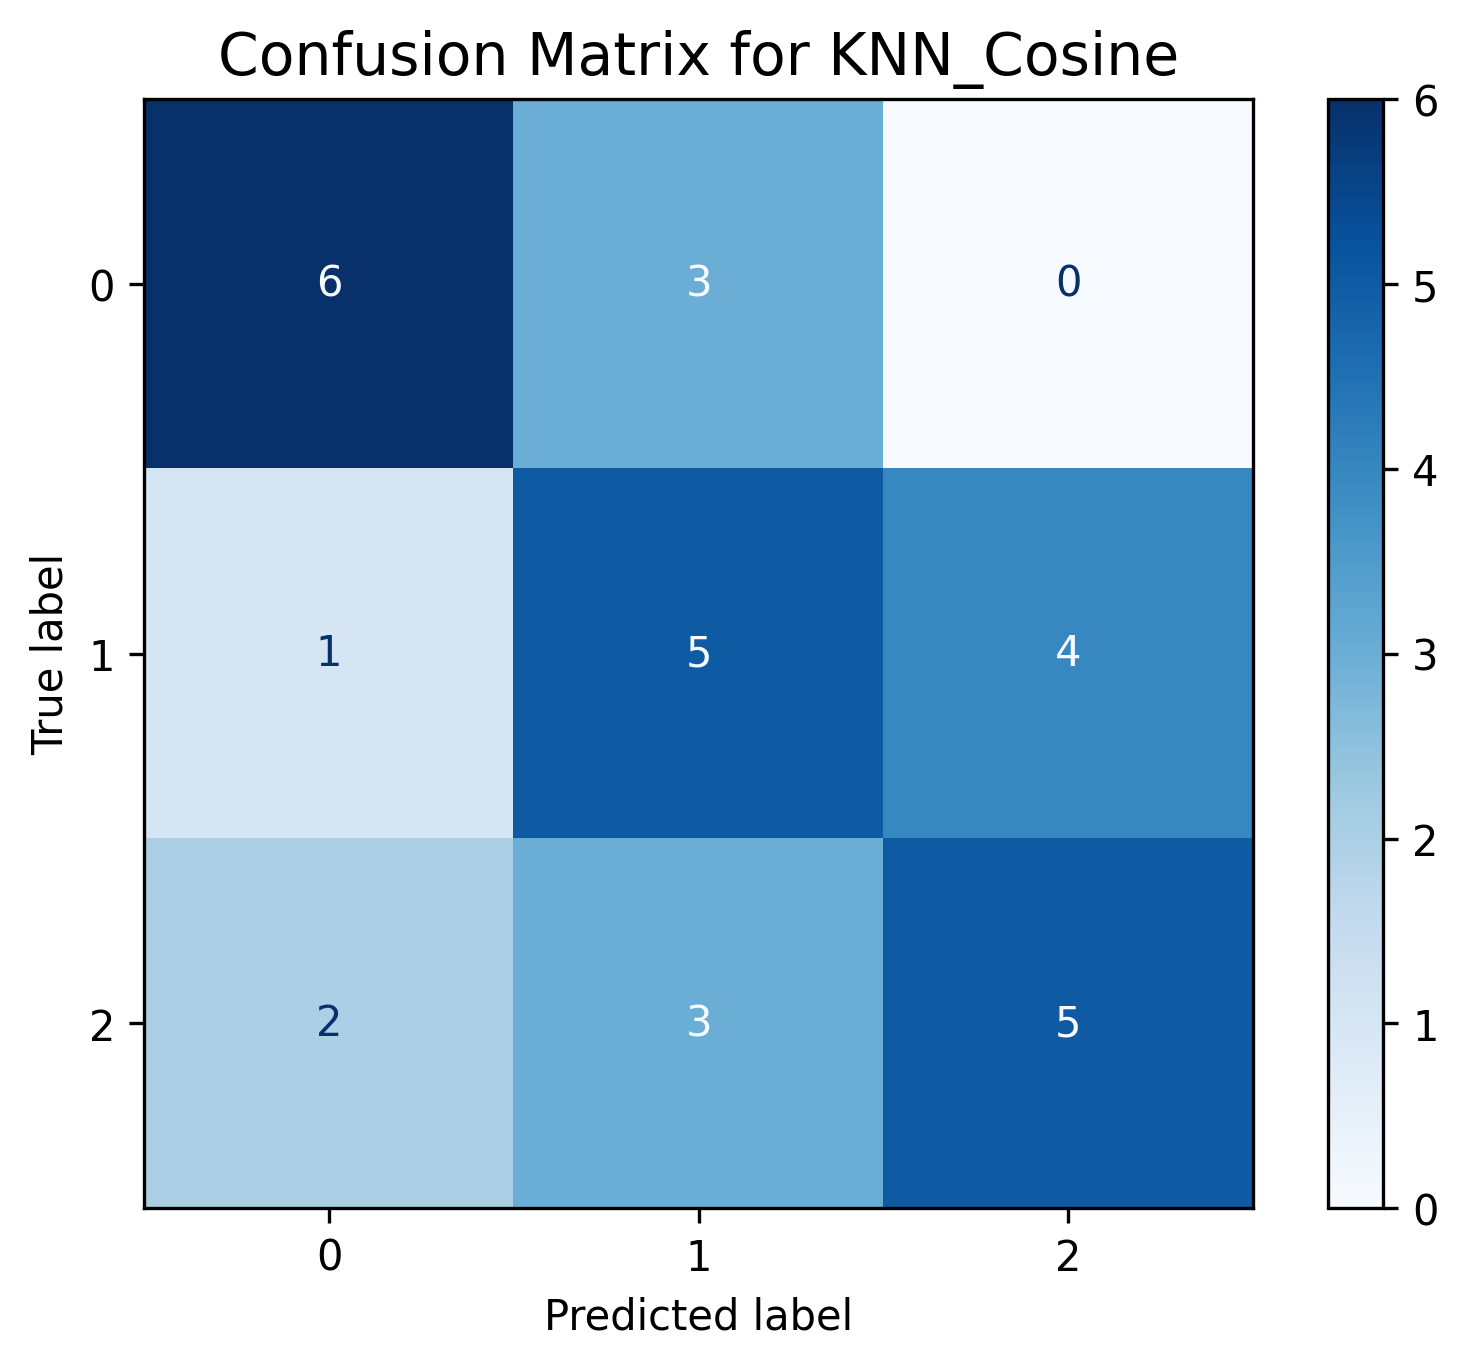
\includegraphics[width=\textwidth]{code/ResultsMainAugZip/plots/Block3_Probabilistic_Experiment_II/confusion_matrix_KNN_Cosine.png}
            \captionof{figure}{Confusion Matrix}
        \end{column}
        \begin{column}{0.33\textwidth}
            \centering
            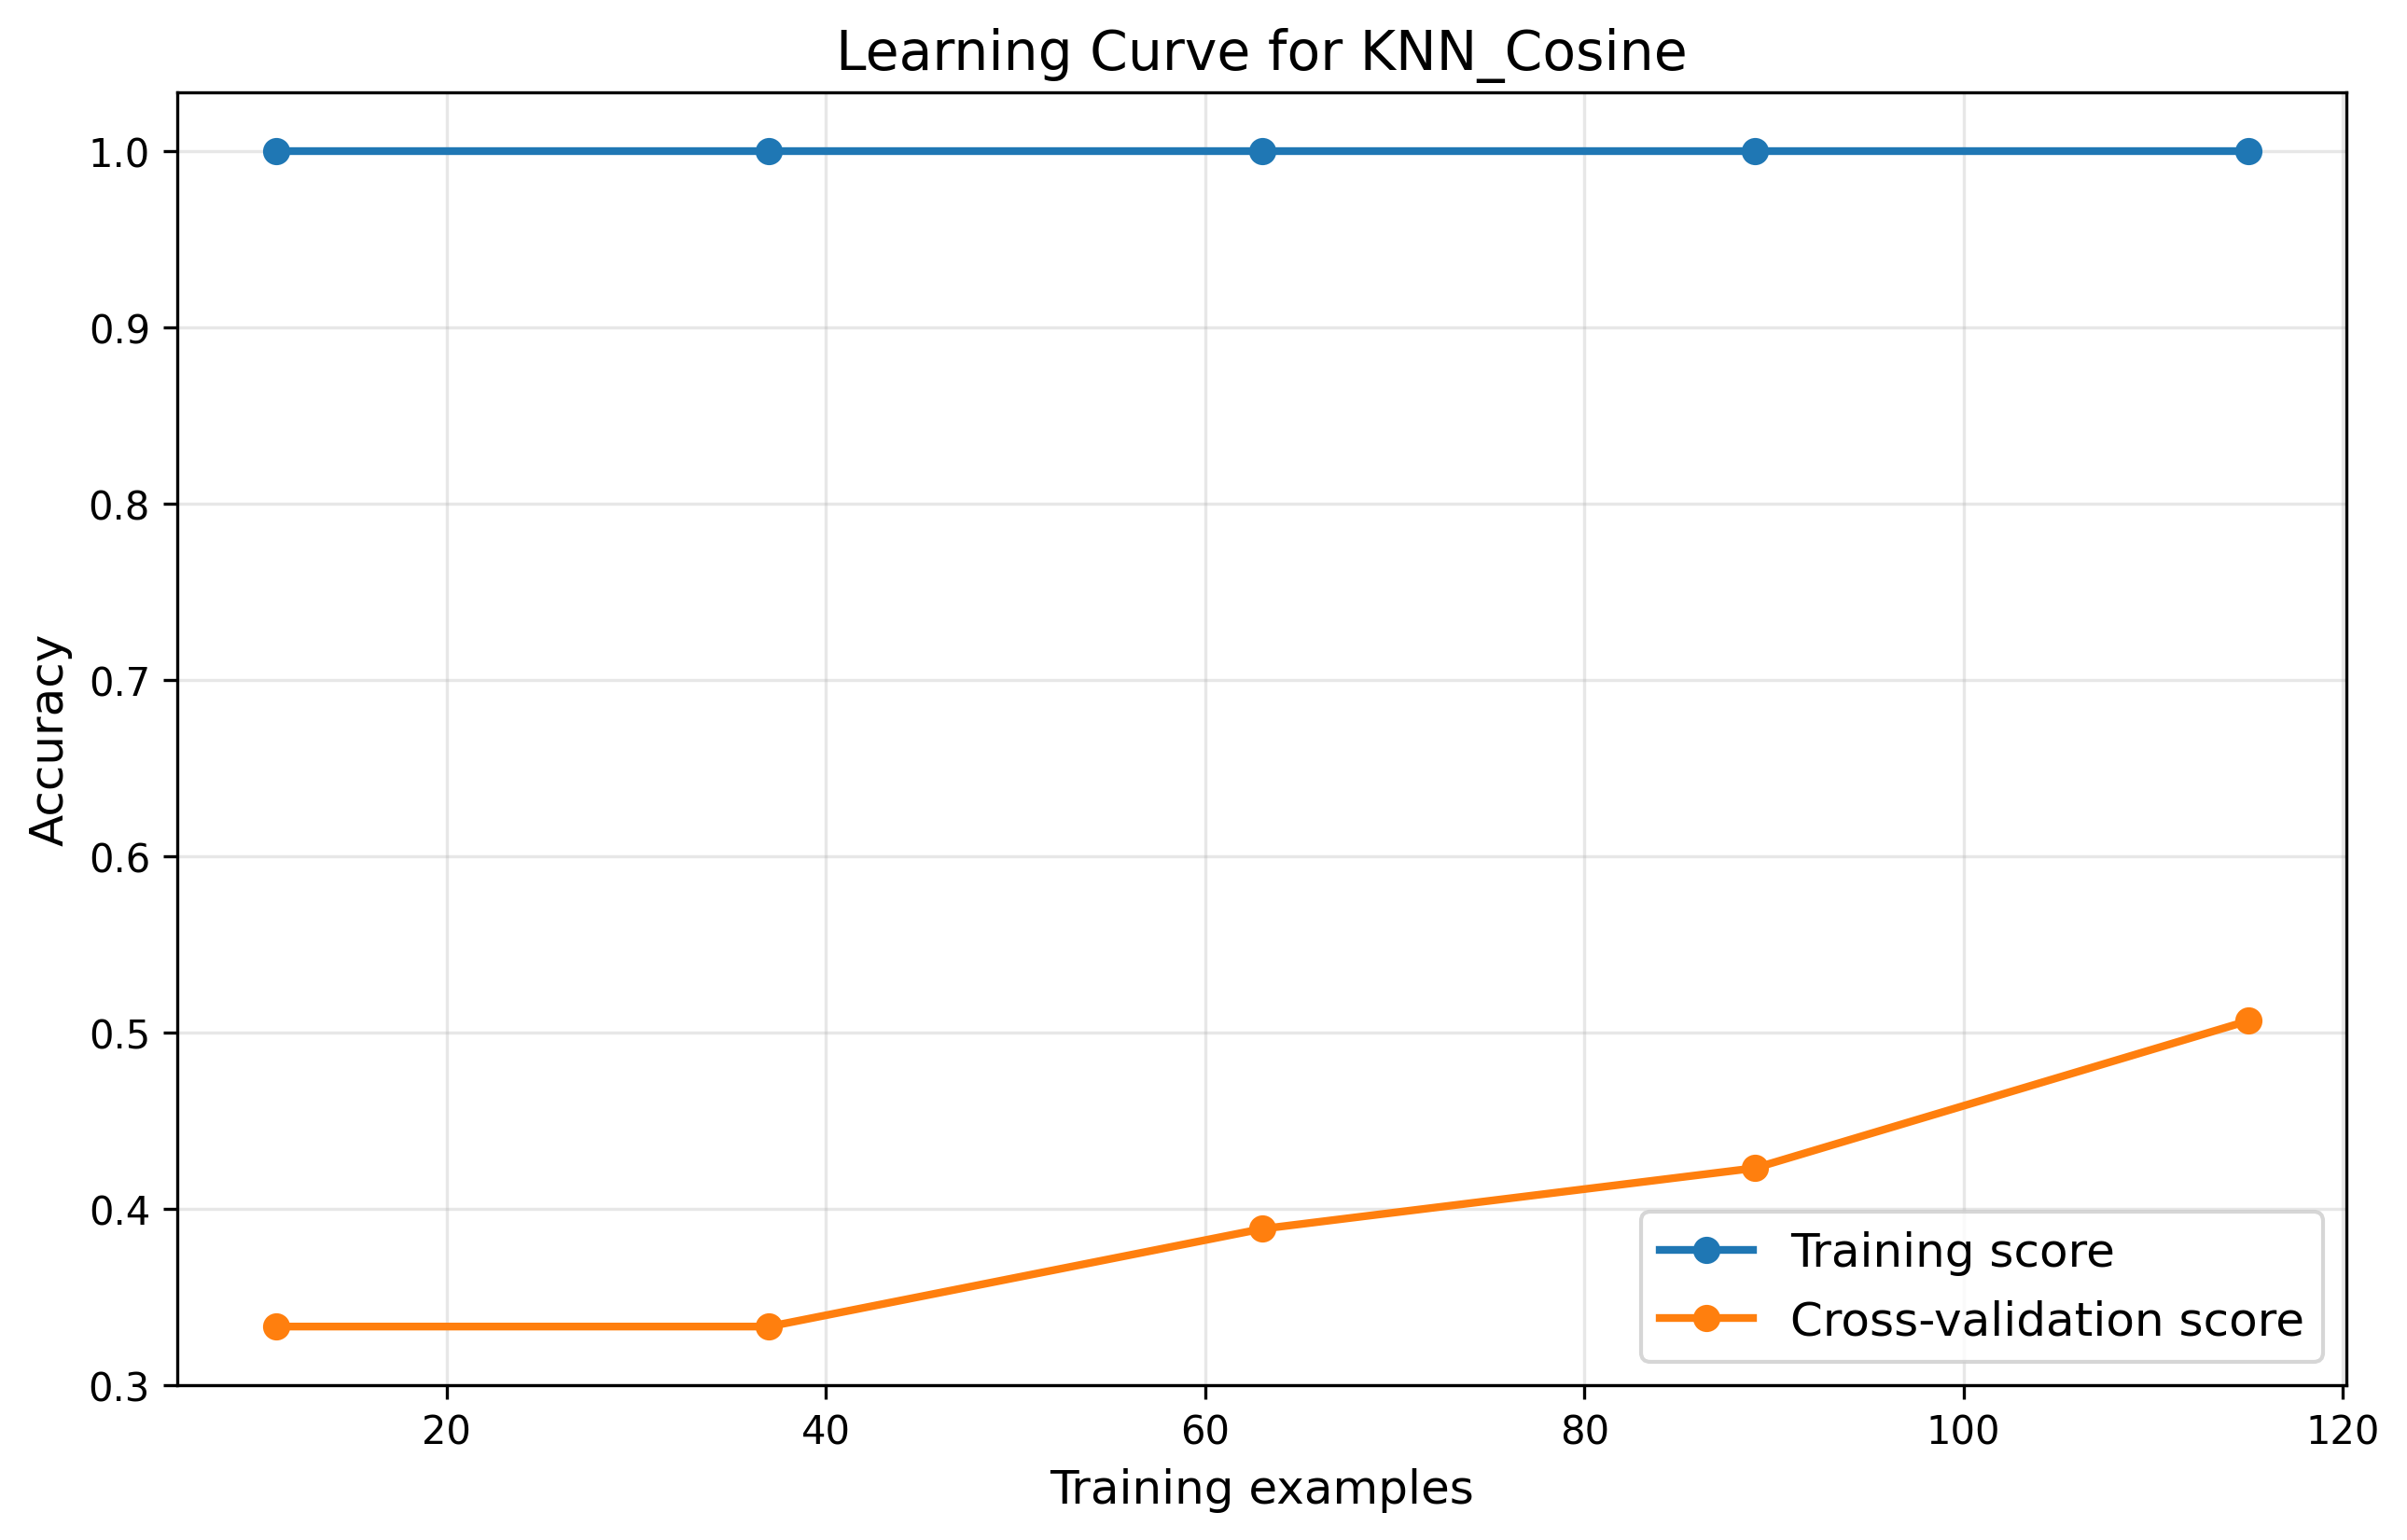
\includegraphics[width=\textwidth]{code/ResultsMainAugZip/plots/Block3_Probabilistic_Experiment_II/learning_curve_KNN_Cosine.png}
            \captionof{figure}{Learning Curve}
        \end{column}
        \begin{column}{0.33\textwidth}
            \centering
            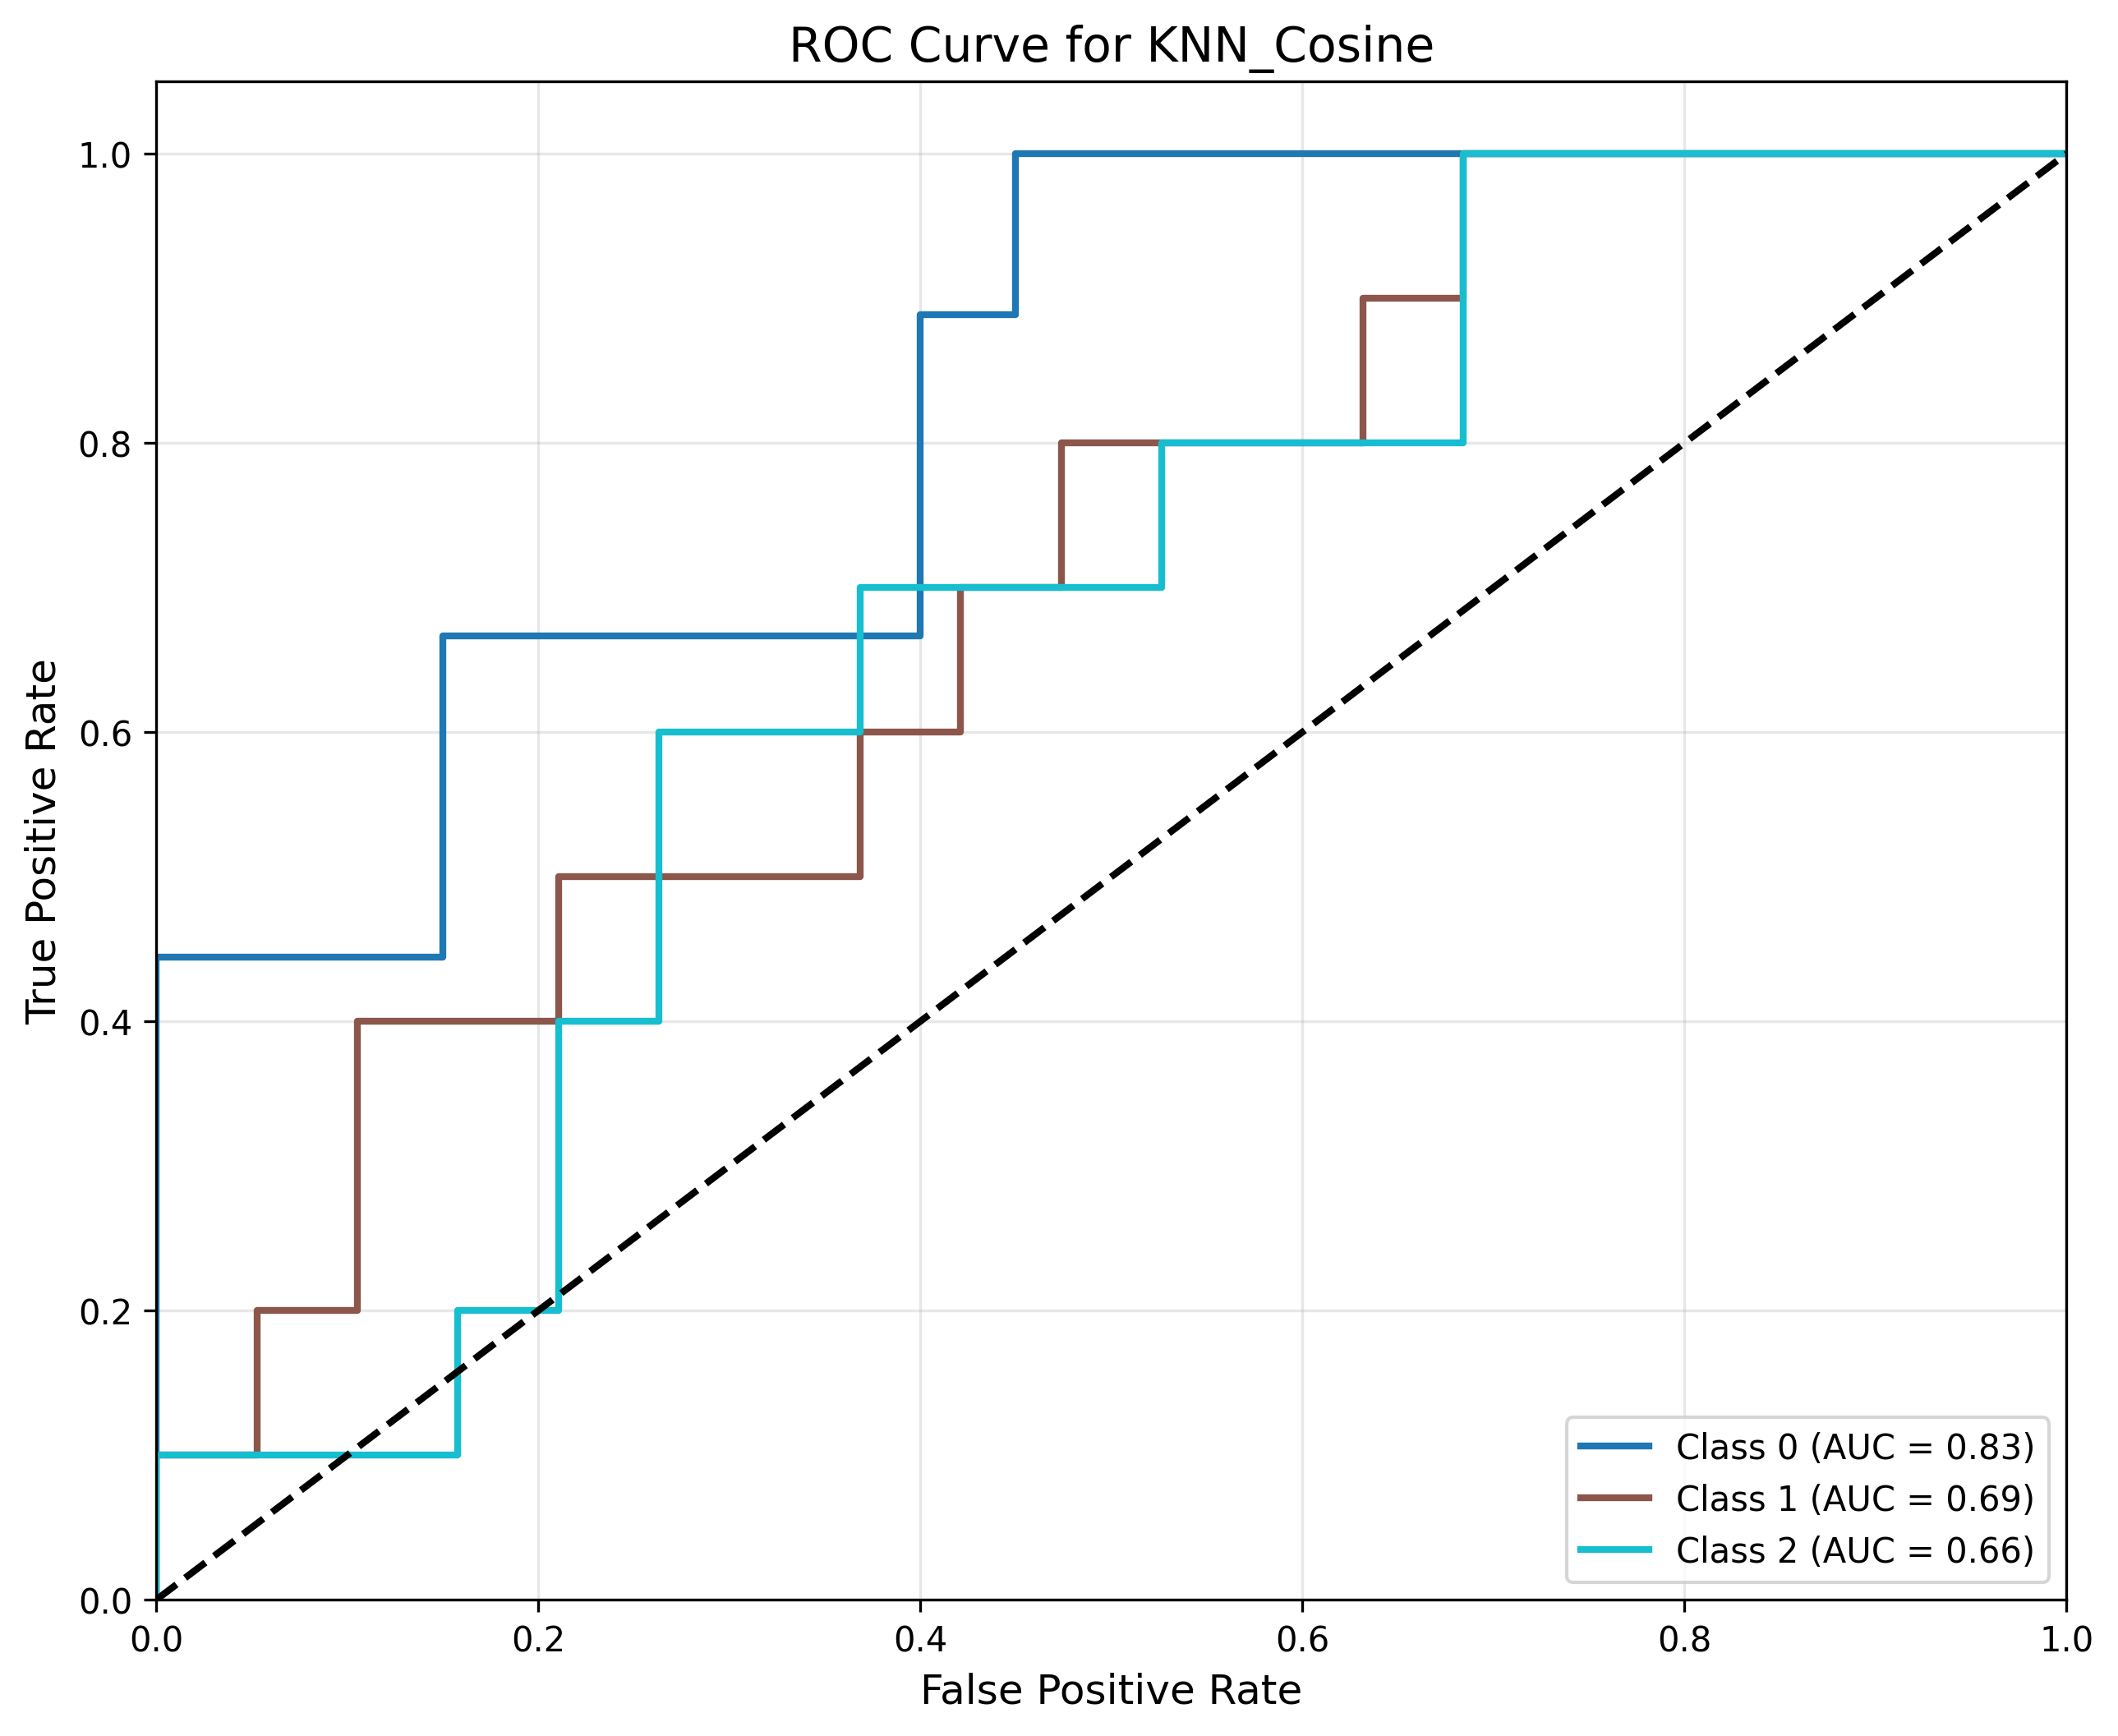
\includegraphics[width=\textwidth]{code/ResultsMainAugZip/plots/Block3_Probabilistic_Experiment_II/roc_curve_KNN_Cosine.png}
            \captionof{figure}{ROC Curve}
        \end{column}
    \end{columns}
    \end{frame}
    
    % Block 4: SVM Variants (Experiment II)
    \begin{frame}{Block 4: SVM Variants (Experiment II)}
    \framesubtitle{Best Model: Linear SVM}
    \begin{columns}
        \begin{column}{0.5\textwidth}
            \centering
            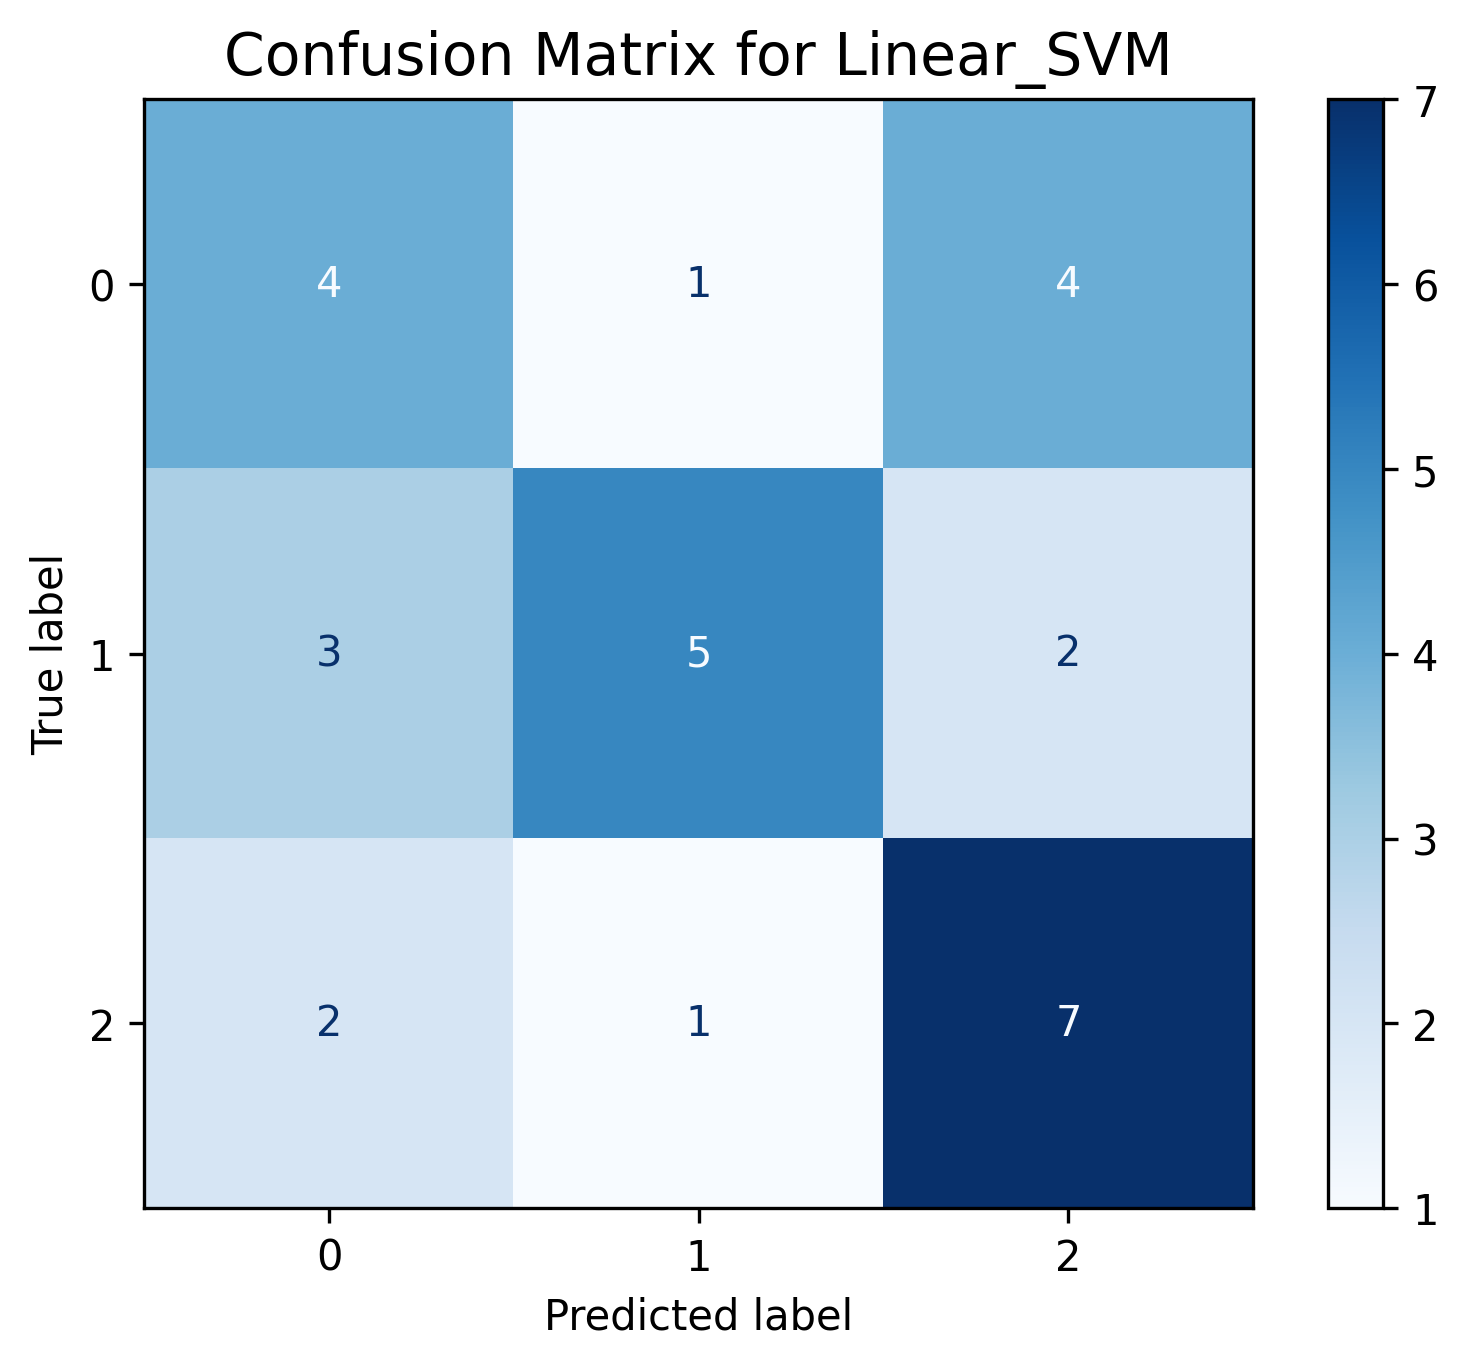
\includegraphics[width=0.9\textwidth]{code/ResultsMainAugZip/plots/Block4_SVM_Variants_Experiment_II/confusion_matrix_Linear_SVM.png}
            \captionof{figure}{Confusion Matrix}
        \end{column}
        \begin{column}{0.5\textwidth}
            \centering
            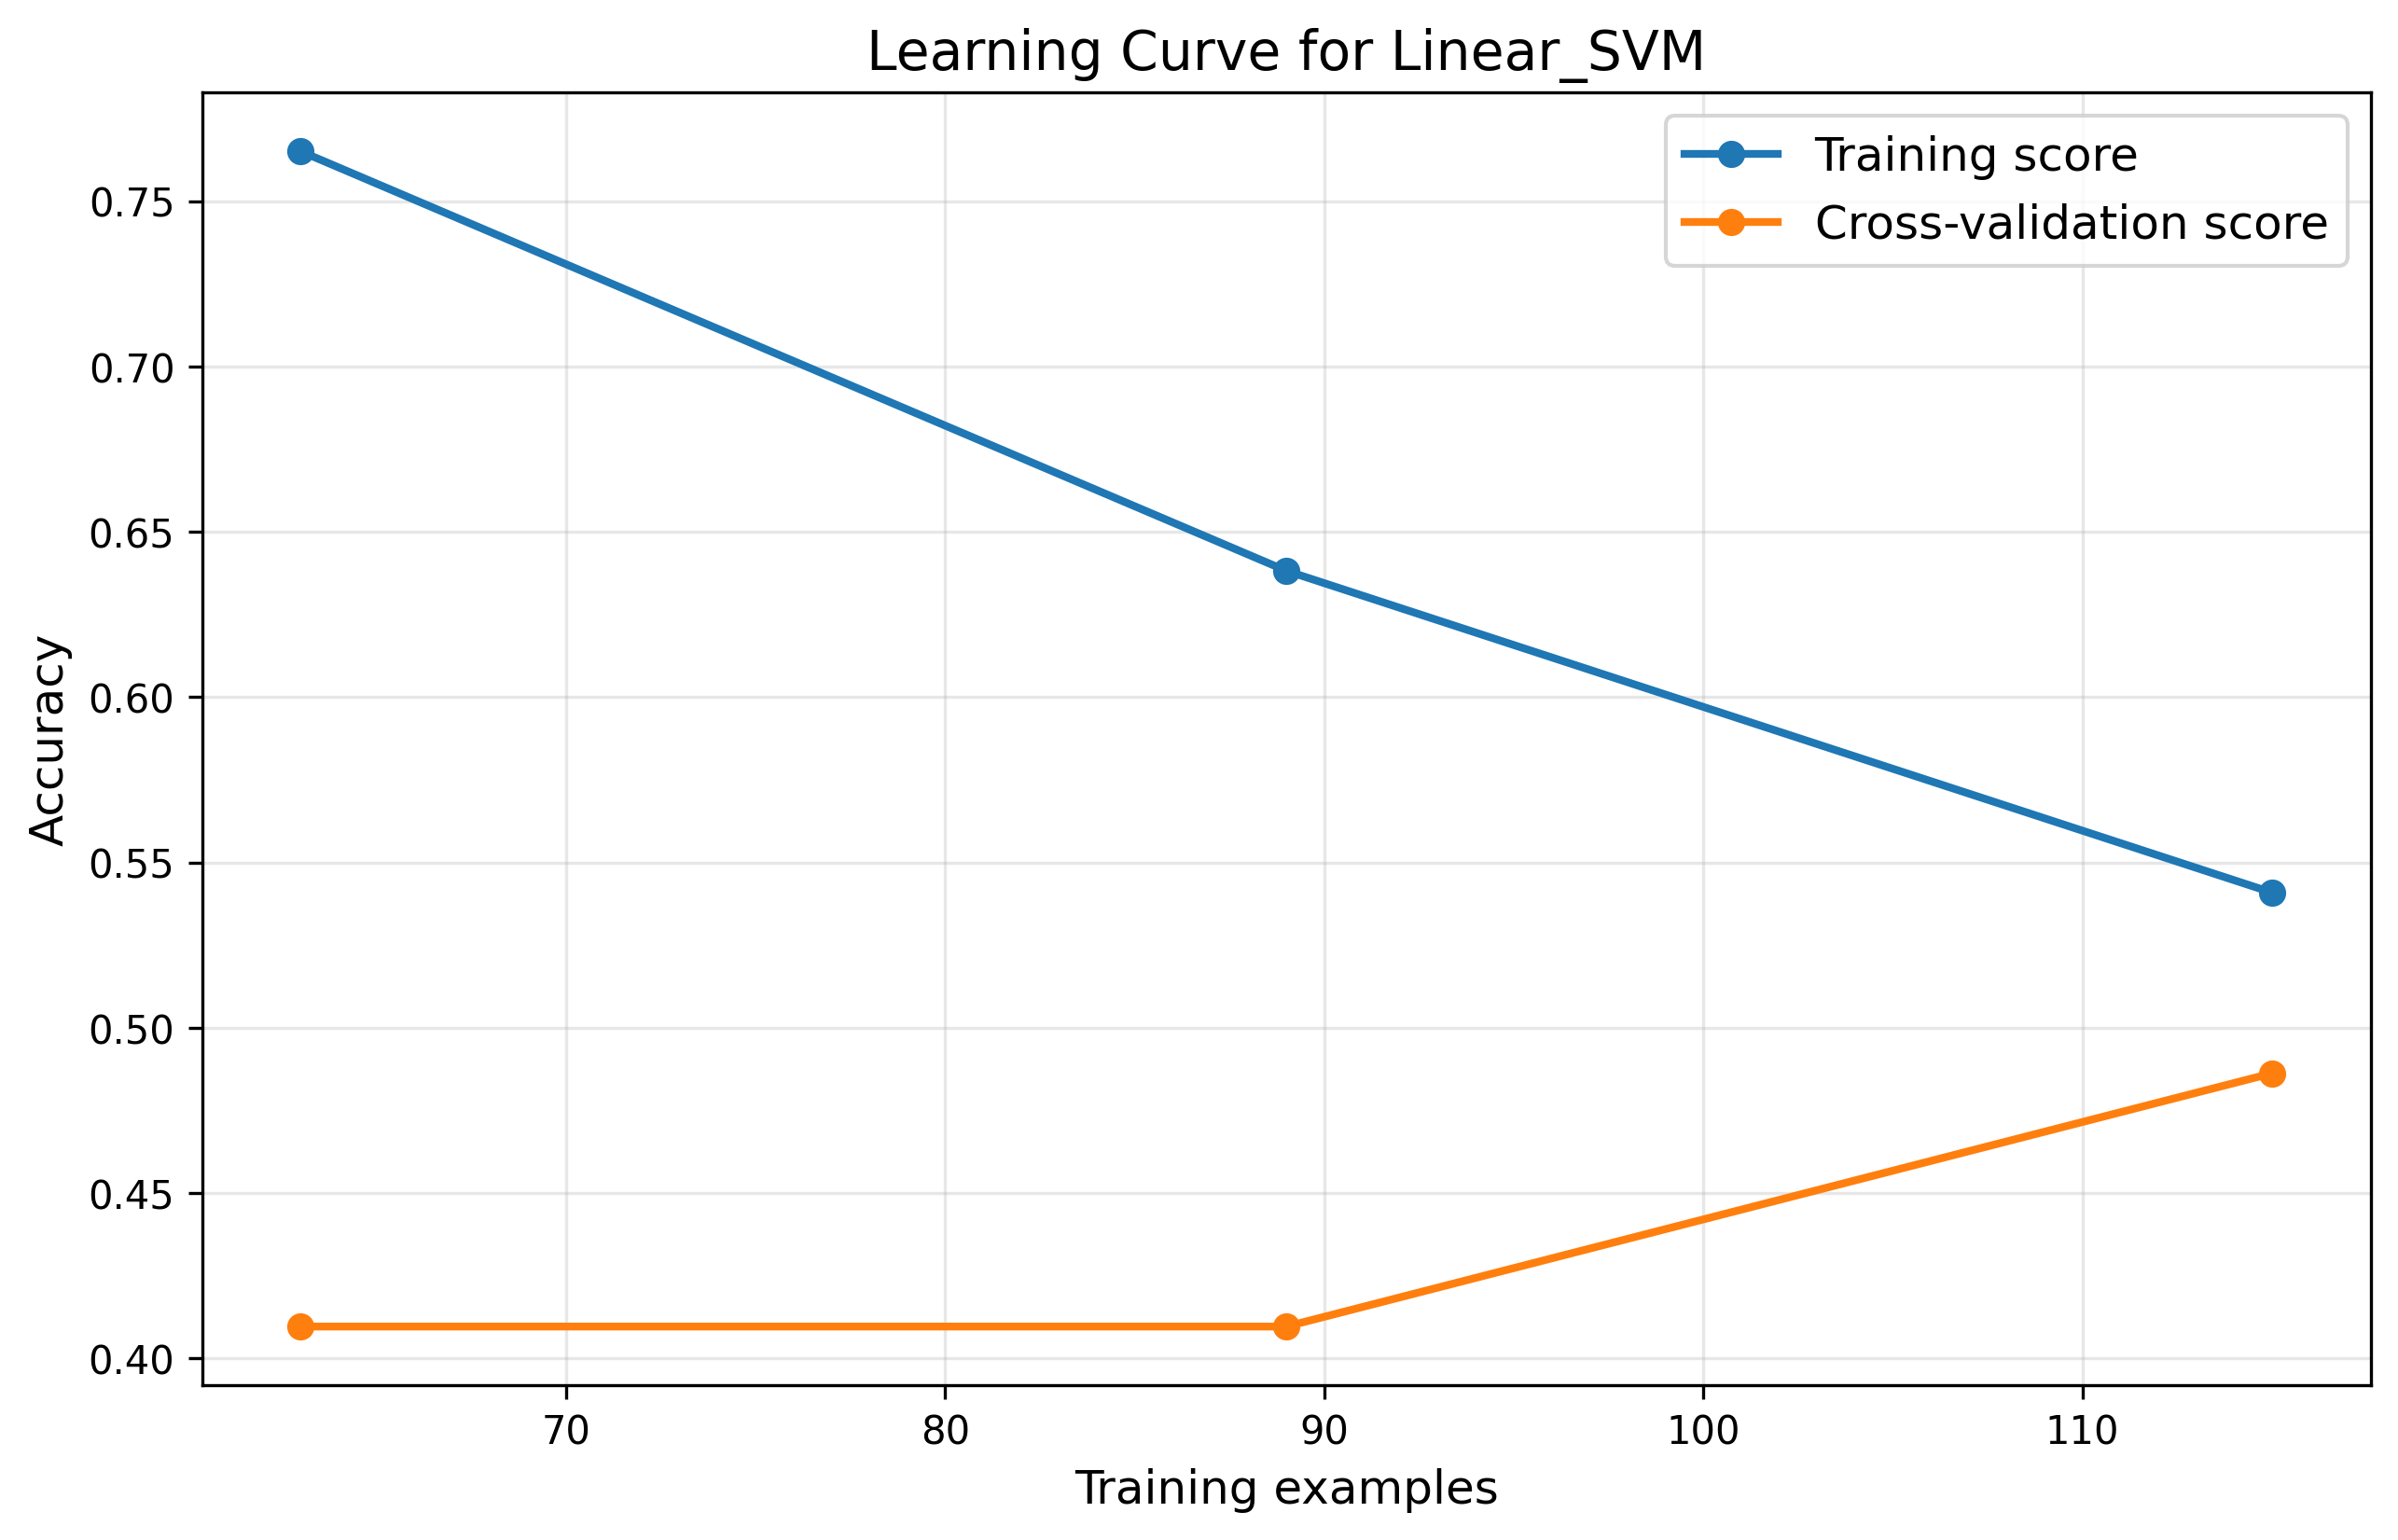
\includegraphics[width=0.9\textwidth]{code/ResultsMainAugZip/plots/Block4_SVM_Variants_Experiment_II/learning_curve_Linear_SVM.png}
            \captionof{figure}{Learning Curve}
        \end{column}
    \end{columns}
    \end{frame}

\end{document}
